% =====================================================================
%  Anatomía de un LLM — Fase IV — Módulo 19
%  Inferencia y generación
%  Compilar: latexmk -r ../latexmkrc M19-inferencia.tex
% =====================================================================
\documentclass[11pt,a4paper,twoside,openany]{book}
\usepackage{../estilo-apuntes}

\newcommand{\ApuntesCurso}{Anatomía de un LLM}
\newcommand{\ApuntesModulo}{Módulo 19}

% Notación propia del módulo
\newcommand{\T}{^{\top}}
\newcommand{\argmax}{\operatorname*{arg\,max}}
\newcommand{\TV}{\operatorname{TV}}
\newcommand{\rnd}{\operatorname{round}}
\newcommand{\clip}{\operatorname{clip}}
\newcommand{\quant}{\operatorname{quant}}
\newcommand{\diag}{\operatorname{diag}}
\newcommand{\Var}{\operatorname{Var}}
\newcommand{\Bmem}{B_{\mathrm{mem}}}
\newcommand{\Ppico}{P_{\mathrm{pico}}}
\newcommand{\Icrit}{I^{\ast}}
\newcommand{\nkv}{n_{\mathrm{kv}}}
\newcommand{\dhd}{d_{\mathrm{h}}}
\newcommand{\TTFT}{\mathrm{TTFT}}
\newcommand{\TPOT}{\mathrm{TPOT}}
\usetikzlibrary{patterns}
\makeatletter\g@addto@macro\UrlBreaks{\do\-}\makeatother

\hypersetup{pdftitle={Módulo 19. Inferencia y generación},pdfauthor={Anatomía de un LLM}}

\begin{document}
\frontmatter
% ------------------------------------------------------------------ Portada
\begin{titlepage}
\centering
\vspace*{2.5cm}
{\large\scshape Anatomía de un LLM}\par
\vspace{0.4cm}
{\normalsize Fundamentos matemáticos de los modelos de lenguaje}\par
\vspace{2.2cm}
\rule{\textwidth}{0.8pt}\par\vspace{0.5cm}
{\small\scshape Fase IV \textperiodcentered\ Escala, sistemas y arquitecturas modernas}\par\vspace{0.3cm}
{\Huge\bfseries Módulo 19\par}\vspace{0.3cm}
{\LARGE Inferencia y generación\par}
\vspace{0.2cm}
{\large Decodificación, caché KV, decodificación especulativa, cuantización y servicio a escala\par}
\vspace{0.5cm}\rule{\textwidth}{0.4pt}\par
\vspace{1.6cm}
{\large Apuntes del curso}\par
\vfill
{\small Edición de octubre de 2026}\par
\end{titlepage}

% ------------------------------------------------------- Presentación
\chapter*{Presentación del módulo}
\addcontentsline{toc}{chapter}{Presentación del módulo}
\markboth{Presentación del módulo}{}

Un modelo de lenguaje entrenado es una distribución condicionada $P(x_t\mid x_{<t})$; para producir texto hay que decidir qué token se emite en cada paso y hacerlo deprisa, para miles de usuarios a la vez y con una memoria limitada. Este módulo estudia ambas cuestiones. La primera es estadística: qué regla de decodificación se aplica a la distribución del modelo (búsqueda voraz, búsqueda en haz, muestreo con temperatura, \emph{top-k} o núcleo) y qué propiedades tiene cada una. La segunda es de sistemas: por qué la generación token a token está limitada por el ancho de banda de memoria y no por el cómputo, cómo la caché de claves y valores evita recalcular el pasado, cómo la decodificación especulativa emite varios tokens por pasada sin alterar la distribución, cómo la cuantización reduce los bytes que hay que leer y cómo se organiza un servidor que atiende muchas peticiones simultáneas. Sobre la inferencia de Claude, Gemini y Grok solo se usa información pública: sus API documentan parámetros de muestreo, pero los formatos numéricos, el hardware y los planificadores con los que se sirven no son públicos.

\section*{Objetivos}
Al finalizar el módulo, el estudiante debe ser capaz de:
\begin{enumerate}[label=\arabic*.]
  \item formular la decodificación como búsqueda o como muestreo, demostrar las propiedades de la temperatura, de \emph{top-k} y del muestreo de núcleo, y aplicar la búsqueda en haz con normalización por longitud;
  \item distinguir las fases de \emph{prefill} y de decodificación, demostrar que la caché KV no altera la salida, calcular su tamaño y deducir con el modelo \emph{roofline} la cota de velocidad de la generación y el efecto del tamaño del lote;
  \item enunciar el algoritmo de decodificación especulativa, demostrar que preserva exactamente la distribución del modelo objetivo y calcular el número esperado de tokens por pasada y la aceleración;
  \item definir la cuantización afín y la simétrica, acotar su error, relacionar bits y relación señal-ruido y analizar el efecto de la granularidad y de los valores atípicos;
  \item explicar y justificar los métodos de cuantización de LLM (LLM.int8(), SmoothQuant, GPTQ, AWQ y QLoRA) y la destilación de conocimiento;
  \item razonar sobre latencia y rendimiento de un servidor, y analizar el \emph{batching} continuo y la gestión paginada de la caché KV.
\end{enumerate}

\section*{Requisitos previos}
Del módulo~1 se usan la regla de la cadena, la función softmax con temperatura y los métodos de muestreo elementales; del módulo~5, esperanza, varianza y distribuciones discretas; del módulo~6, entropía y entropía cruzada; del módulo~11, los formatos de coma flotante; de los módulos~13 a~15, la atención causal, el bloque Transformer y el mini-GPT; del módulo~16, el coste de unas $2N$ operaciones por token en la pasada hacia delante; del módulo~17, la intensidad aritmética y el modelo \emph{roofline}, y del módulo~18, la atención con consultas agrupadas (GQA).

\section*{Organización}
\begin{center}\small
\begin{tabular}{@{}cll@{}}
\toprule
Tema & Contenido & Fuentes principales \\
\midrule
1 & Decodificación: búsqueda y muestreo & \cite{jm3}, \cite{d2l}, \cite{holtzman}, \cite{fan} \\
2 & Coste de la inferencia y caché KV & \cite{cs336}, \cite{pope}, \cite{kwon}, \cite{shazeer} \\
3 & Decodificación especulativa & \cite{leviathan}, \cite{chen}, \cite{cs336} \\
4 & Fundamentos de la cuantización & \cite{grayneuhoff}, \cite{jacob}, \cite{mit65940}, \cite{smoothquant} \\
5 & Cuantización de LLM y destilación & \cite{llmint8}, \cite{smoothquant}, \cite{gptq}, \cite{awq}, \cite{qlora}, \cite{hinton} \\
6 & Servicio a escala: latencia, rendimiento y memoria & \cite{cs336}, \cite{orca}, \cite{kwon}, \cite{pope} \\
\bottomrule
\end{tabular}
\end{center}

Cada tema termina con una lista de lecturas y con ejercicios graduados en tres niveles: $\star$ comprensión, $\star\star$ cálculo y $\star\star\star$ demostración. Los ejercicios marcados con \emph{Fuente} están adaptados de cursos y libros de texto universitarios; el enunciado se ha redactado de nuevo y, en algunos casos, se han cambiado los datos para que puedan resolverse a mano. Las soluciones completas, paso a paso, están en el \cref{ap:soluciones}.

\section*{Sobre las fuentes}
El texto es de redacción propia. La organización sigue la clase~10 («Inference») del curso CS336 de Stanford, «Language Modeling from Scratch»~\cite{cs336}, que recorre la intensidad aritmética de la inferencia, la caché KV, la cuantización, la decodificación especulativa, el \emph{batching} continuo y PagedAttention, y la sección~6 de su tarea~1~\cite{cs336a1}, dedicada a la generación. La decodificación sigue el §7.6 y el §13.4 de Jurafsky y Martin~\cite{jm3} y el §10.8 de Zhang \emph{et al.}~\cite{d2l}. La cuantización sigue las clases~5 y~6 («Quantization»), 9 («Knowledge Distillation») y~13 («Efficient LLM Deployment») del curso 6.5940 del MIT~\cite{mit65940}, el estudio clásico de Gray y Neuhoff~\cite{grayneuhoff} y el esquema de aritmética entera de Jacob \emph{et al.}~\cite{jacob}. Los métodos se toman de sus artículos originales: Holtzman \emph{et al.}~\cite{holtzman} y Fan \emph{et al.}~\cite{fan} para el muestreo; Pope \emph{et al.}~\cite{pope} y Shazeer~\cite{shazeer} para el coste de la inferencia; Leviathan \emph{et al.}~\cite{leviathan} y Chen \emph{et al.}~\cite{chen} para la decodificación especulativa; Dettmers \emph{et al.}~\cite{llmint8,qlora}, Xiao \emph{et al.}~\cite{smoothquant}, Frantar \emph{et al.}~\cite{gptq} y Lin \emph{et al.}~\cite{awq} para la cuantización; Hinton \emph{et al.}~\cite{hinton} para la destilación, y Yu \emph{et al.}~\cite{orca} y Kwon \emph{et al.}~\cite{kwon} para el servicio. Las arquitecturas que se usan como ejemplo (Llama~2, Llama~3, OPT) son públicas; sobre los modelos comerciales (Claude, Gemini, Grok) solo se usa información pública.

\section*{Notación}
\begin{center}\small
\begin{tabularx}{\textwidth}{@{}l>{\raggedright\arraybackslash}X@{}}
\toprule
Símbolo & Significado \\
\midrule
$\V$, $K=\abs{\V}$ & vocabulario y su tamaño \\
$x_{<t}=(x_1,\dots,x_{t-1})$ & prefijo (contexto) en el paso $t$ \\
$z\in\R^{K}$, $\tau>0$ & vector de logits y temperatura (la letra $T$ se reserva para longitudes) \\
$p_\tau=\softmax(z/\tau)$ & distribución con temperatura \\
$k$, $p$, $m$ & parámetros de \emph{top-k}, del muestreo de núcleo y anchura del haz \\
$N$, $n$ & parámetros del modelo y longitud del prompt \\
$L$, $\nkv$, $\dhd$ & capas, cabezas de clave y valor, y dimensión de cada cabeza \\
$s$ & bytes por número (2 en fp16 y bf16, 1 en int8) \\
$B$, $\Bmem$, $\Ppico$ & tamaño del lote, ancho de banda de memoria y rendimiento máximo \\
$p$, $q$ & en el tema~3, distribución del modelo objetivo y del borrador \\
$\gamma$, $\beta$, $\alpha$, $c$ & tokens propuestos, tasa de aceptación, su valor esperado y coste relativo del borrador \\
$\TV(p,q)$ & distancia de variación total, $\frac12\sum_x\abs{p(x)-q(x)}$ \\
$b$, $\Delta$, $Z$ & bits, paso (escala) y punto cero de un cuantizador \\
$H=2XX\T$ & matriz hessiana del error cuadrático de una capa (tema~5) \\
$\TTFT$, $\TPOT$ & tiempo hasta el primer token y tiempo por token de salida \\
\bottomrule
\end{tabularx}
\end{center}

\tableofcontents

\mainmatter
% =====================================================================
\chapter{Decodificación: búsqueda y muestreo}
\label{tema:1}
% =====================================================================

Un modelo de lenguaje autorregresivo proporciona, en cada paso, una distribución $P(\cdot\mid x_{<t})$ sobre el vocabulario; la \emph{decodificación} es la regla que convierte esa sucesión de distribuciones en un texto concreto. Este tema presenta las dos familias de reglas: las de \emph{maximización} (búsqueda voraz y búsqueda en haz), que intentan encontrar la secuencia más probable, y las de \emph{muestreo} (temperatura, \emph{top-k} y núcleo), que extraen una secuencia aleatoria de una versión modificada de la distribución. Se siguen el §7.6 y el §13.4 de Jurafsky y Martin~\cite{jm3}, el §10.8 de Zhang \emph{et al.}~\cite{d2l}, la sección~3 de Holtzman \emph{et al.}~\cite{holtzman}, el §5.4 de Fan \emph{et al.}~\cite{fan} y la sección~6 de la tarea~1 de CS336~\cite{cs336a1}.

\section{El problema de la decodificación}

Sea $P$ un modelo de lenguaje sobre $\V$ con símbolo de fin \fin\ (módulo~1). Por la regla de la cadena, la probabilidad de una continuación $y=(y_1,\dots,y_T)$ de un prompt $x$ es
\[
P(y\mid x)=\prod_{t=1}^{T}P(y_t\mid x,y_{<t}),\qquad
\ln P(y\mid x)=\sum_{t=1}^{T}\ln P(y_t\mid x,y_{<t}).
\]

\begin{definicion}[Regla de decodificación]\label{def:decodificacion}
Una \emph{regla de decodificación} es un procedimiento que, a partir del prompt $x$ y del acceso a las distribuciones condicionadas $P(\cdot\mid x,y_{<t})$, produce una continuación $y$, de forma determinista o aleatoria. La \emph{decodificación de máxima probabilidad} (MAP) busca
\[
y^{\ast}=\argmax_{y}\ P(y\mid x),
\]
donde el máximo se toma sobre las secuencias terminadas en \fin.
\end{definicion}

\begin{proposicion}\label{prop:exhaustiva}
Con un vocabulario de $K$ tokens, el número de continuaciones de longitud exactamente $T$ es $K^{T}$. En consecuencia, la búsqueda exhaustiva del máximo entre las secuencias de longitud $T$ requiere evaluar $K^{T}$ secuencias.
\end{proposicion}

\begin{proof}
Cada una de las $T$ posiciones admite $K$ tokens de forma independiente; por el principio del producto hay $K^{T}$ secuencias (módulo~1).
\end{proof}

Con $K=5\cdot 10^{4}$ y $T=20$, $K^{T}\approx 9{,}5\cdot 10^{93}$: la decodificación MAP exacta es inabordable y se aproxima con búsquedas locales~\cite[§10.8.2]{d2l}.

\section{Búsqueda voraz y búsqueda en haz}

\begin{definicion}[Búsqueda voraz]
La \emph{búsqueda voraz} (\emph{greedy}) elige en cada paso el token más probable, $y_t=\argmax_{v\in\V}P(v\mid x,y_{<t})$, hasta emitir \fin\ o alcanzar una longitud máxima~\cite[§7.6.1]{jm3}.
\end{definicion}

\begin{proposicion}\label{prop:voraz-no-optima}
La búsqueda voraz no encuentra, en general, la secuencia de máxima probabilidad.
\end{proposicion}

\begin{proof}
Basta un contraejemplo. Sea un modelo con primer token $A$, $B$ o $C$, con probabilidades $0{,}5$, $0{,}4$ y $0{,}1$, y segundo token $\mathrm{x}$, $\mathrm{y}$ o $\mathrm{z}$ seguido de \fin. Tras $A$ el segundo token tiene distribución $(0{,}4;\allowbreak\,0{,}3;\allowbreak\,0{,}3)$ y tras $B$, $(0{,}9;\allowbreak\,0{,}05;\allowbreak\,0{,}05)$. La búsqueda voraz elige $A$ y luego $\mathrm{x}$, con probabilidad $0{,}5\cdot 0{,}4=0{,}20$, mientras que la secuencia $B\mathrm{x}$ tiene probabilidad $0{,}4\cdot 0{,}9=0{,}36>0{,}20$.
\end{proof}

\begin{definicion}[Búsqueda en haz]\label{def:haz}
Sea $m\ge 1$ la \emph{anchura del haz}. La \emph{búsqueda en haz} mantiene un conjunto $\mathcal{H}_t$ de, a lo sumo, $m$ prefijos de longitud $t$. En el paso $t+1$ forma todas las extensiones $(h,v)$ con $h\in\mathcal{H}_t$ y $v\in\V$, las puntúa con $\ln P(h,v\mid x)=\ln P(h\mid x)+\ln P(v\mid x,h)$ y conserva las $m$ de mayor puntuación. Las extensiones que terminan en \fin\ se retiran del haz como candidatas finales; al acabar se devuelve la candidata de mayor puntuación~\cite[§13.4]{jm3}, \cite[§10.8.3]{d2l}.
\end{definicion}

\begin{figure}[h]
\centering
\begin{tikzpicture}[font=\small,
  nodo/.style={draw,rounded corners=2pt,minimum width=9mm,minimum height=6mm},
  poda/.style={nodo,dashed,draw=regla,text=regla},
  level distance=1.9cm]
  \node[nodo] (r) at (0,0) {\fin};
  \node[nodo] (A) at (2.6,1.4) {$A$};
  \node[nodo] (B) at (2.6,0) {$B$};
  \node[poda] (C) at (2.6,-1.4) {$C$};
  \draw[->] (r) -- node[above,sloped] {$0{,}5$} (A);
  \draw[->] (r) -- node[above] {$0{,}4$} (B);
  \draw[->,regla] (r) -- node[below,sloped] {$0{,}1$} (C);
  \node[nodo] (Ax) at (6.2,2.1) {$A\mathrm{x}$: $0{,}20$};
  \node[poda] (Ay) at (6.2,1.4) {$A\mathrm{y}$: $0{,}15$};
  \node[nodo] (Bx) at (6.2,0.35) {$B\mathrm{x}$: $0{,}36$};
  \node[poda] (By) at (6.2,-0.35) {$B\mathrm{y}$: $0{,}02$};
  \draw[->] (A) -- (Ax); \draw[->,regla] (A) -- (Ay);
  \draw[->] (B) -- (Bx); \draw[->,regla] (B) -- (By);
  \node[align=left,font=\footnotesize,anchor=west] at (8.0,1.0) {haz $m=2$:\\ se conservan $A\mathrm{x}$ y $B\mathrm{x}$;\\ gana $B\mathrm{x}$};
\end{tikzpicture}
\caption{Búsqueda en haz con $m=2$ en el ejemplo de la \cref{prop:voraz-no-optima}. Los nodos discontinuos se podan (no se dibujan las extensiones con $\mathrm{z}$). La búsqueda voraz se queda con $A\mathrm{x}$ ($0{,}20$); el haz encuentra $B\mathrm{x}$ ($0{,}36$).}
\label{fig:haz}
\end{figure}

\begin{proposicion}[Coste y casos extremos]\label{prop:coste-haz}
Para una salida de longitud $T$ y vocabulario de tamaño $K$, la búsqueda en haz de anchura $m$ evalúa a lo sumo $mKT$ extensiones. Con $m=1$ coincide con la búsqueda voraz, y con $m\ge K^{T-1}$ no poda ningún prefijo y coincide con la búsqueda exhaustiva entre las secuencias de longitud~$T$.
\end{proposicion}

\begin{proof}
En cada uno de los $T$ pasos se extienden a lo sumo $m$ prefijos con $K$ tokens. Si $m=1$, conservar la mejor extensión del único prefijo es elegir el $\argmax$ del paso, que es la regla voraz. En el paso $t$ hay a lo sumo $K^{t}\le K^{T-1}$ prefijos posibles para $t\le T-1$; si $m\ge K^{T-1}$, ninguno se descarta y en el último paso se puntúan las $K^{T}$ secuencias.
\end{proof}

\begin{observacion}[Sesgo hacia las secuencias cortas]\label{obs:longitud}
Cada término $\ln P(y_t\mid x,y_{<t})$ es menor o igual que cero, de modo que la puntuación $\ln P(y\mid x)$ no aumenta al alargar la secuencia. La búsqueda en haz tiende entonces a preferir candidatas cortas. La corrección habitual divide por una potencia de la longitud,
\[
\mathrm{punt}(y)=\frac{1}{L^{a}}\ln P(y\mid x),\qquad L=\abs{y},\ a\in[0,1],
\]
con $a=0{,}75$ en el ejemplo de~\cite[§10.8.3]{d2l}; con $a=1$ se obtiene la log-probabilidad media por token de~\cite[§13.4]{jm3}.
\end{observacion}

\begin{observacion}[Degeneración]
La búsqueda en haz es la regla habitual en traducción automática, donde la salida está muy determinada por la entrada. En la generación abierta produce textos repetitivos: Holtzman \emph{et al.} muestran que el texto humano tiene una probabilidad por token claramente menor que la del texto obtenido por maximización y que las repeticiones se refuerzan a sí mismas, porque cada repetición aumenta la probabilidad de la siguiente~\cite[§4.3]{holtzman}. Por eso los asistentes conversacionales muestrean.
\end{observacion}

\section{Muestreo con temperatura}

\begin{definicion}[Softmax con temperatura]\label{def:temperatura}
Sea $z\in\R^{K}$ el vector de logits y sea $\tau>0$. La \emph{distribución con temperatura} $\tau$ es
\[
p_\tau(i)=\frac{e^{z_i/\tau}}{\sum_{j=1}^{K}e^{z_j/\tau}},\qquad i=1,\dots,K.
\]
El \emph{muestreo con temperatura} extrae cada token de $p_\tau$~\cite[§7.6.3]{jm3}, \cite[§3.3]{holtzman}. Con $\tau=1$ se recupera la distribución del modelo.
\end{definicion}

\begin{proposicion}[Temperatura como potencia]\label{prop:potencia}
Sea $p=p_1$ la distribución del modelo. Entonces $p_\tau(i)\propto p(i)^{1/\tau}$. En particular, elevar las probabilidades a una potencia $a>0$ y renormalizar equivale a muestrear con temperatura $\tau=1/a$.
\end{proposicion}

\begin{proof}
Como $p(i)=e^{z_i}/\sum_j e^{z_j}$, se tiene $p(i)^{1/\tau}=e^{z_i/\tau}\bigl(\sum_j e^{z_j}\bigr)^{-1/\tau}$. El segundo factor no depende de $i$ y desaparece al normalizar, luego $p(i)^{1/\tau}\big/\sum_j p(j)^{1/\tau}=p_\tau(i)$.
\end{proof}

\begin{proposicion}[Límites de la temperatura]\label{prop:limites-tau}
Sea $M=\{i:z_i=\max_j z_j\}$ el conjunto de logits máximos. Entonces
\[
\lim_{\tau\to 0^{+}}p_\tau(i)=\begin{cases}1/\abs{M}, & i\in M,\\ 0,& i\notin M,\end{cases}
\qquad
\lim_{\tau\to\infty}p_\tau(i)=\frac{1}{K}.
\]
Si el máximo es único, el límite $\tau\to 0^{+}$ es la búsqueda voraz.
\end{proposicion}

\begin{proof}
Sea $z^{\ast}=\max_j z_j$. Multiplicando numerador y denominador por $e^{-z^{\ast}/\tau}$,
\[
p_\tau(i)=\frac{e^{(z_i-z^{\ast})/\tau}}{\sum_{j}e^{(z_j-z^{\ast})/\tau}}.
\]
Cuando $\tau\to 0^{+}$, cada exponente $(z_j-z^{\ast})/\tau$ vale $0$ si $j\in M$ y tiende a $-\infty$ si $j\notin M$; el denominador tiende a $\abs{M}$ y el numerador a $1$ o a $0$. Cuando $\tau\to\infty$, todos los exponentes tienden a $0$, el numerador a $1$ y el denominador a $K$.
\end{proof}

\begin{ejemplo}\label{ej:muestreo}
Sean los logits $z=(2,1,0,-1)$ de los tokens $A,B,C,D$. Con $\tau=1$, $p_1=(0{,}6439;\allowbreak\,0{,}2369;\allowbreak\,0{,}0871;\allowbreak\,0{,}0321)$. Con $\tau=0{,}5$ la distribución se afila, $p_{0{,}5}=(0{,}8650;\allowbreak\,0{,}1171;\allowbreak\,0{,}0158;\allowbreak\,0{,}0021)$, y con $\tau=2$ se aplana, $p_{2}=(0{,}4551;\allowbreak\,0{,}2760;\allowbreak\,0{,}1674;\allowbreak\,0{,}1015)$.
\end{ejemplo}

La temperatura reescala todos los logits por igual y nunca anula un token: la cola de tokens improbables conserva masa positiva para cualquier $\tau>0$. Los métodos de truncamiento la eliminan.

\section{Truncamiento: \emph{top-k} y muestreo de núcleo}

\begin{definicion}[Distribución truncada]\label{def:truncada}
Sea $p$ una distribución sobre $\V$ y sea $S\subseteq\V$ con $p(S)=\sum_{i\in S}p(i)>0$. La \emph{distribución truncada} a $S$ es $p_S(i)=p(i)/p(S)$ si $i\in S$ y $p_S(i)=0$ en otro caso.
\end{definicion}

\begin{definicion}[\emph{Top-k} y núcleo]\label{def:topk-topp}
Sea $p_{(1)}\ge p_{(2)}\ge\dots\ge p_{(K)}$ la ordenación decreciente de las probabilidades.
\begin{enumerate}[label=(\alph*)]
  \item El muestreo \emph{top-k}~\cite[§5.4]{fan} trunca $p$ al conjunto $V^{(k)}$ de los $k$ tokens más probables.
  \item El \emph{muestreo de núcleo} o \emph{top-p}~\cite[§3.1]{holtzman}, con umbral $p\in(0,1]$, trunca al menor conjunto $V^{(p)}$ tal que $\sum_{i\in V^{(p)}}p(i)\ge p$.
\end{enumerate}
\end{definicion}

\begin{proposicion}[El núcleo está formado por los más probables]\label{prop:nucleo}
Sea $k^{\ast}=\min\{k:\sum_{i=1}^{k}p_{(i)}\ge p\}$. Entonces el tamaño mínimo de un conjunto con masa al menos $p$ es $k^{\ast}$, y el conjunto de los $k^{\ast}$ tokens más probables lo alcanza. Es decir, el muestreo de núcleo coincide con \emph{top-k} con $k=k^{\ast}$, donde $k^{\ast}$ depende de la distribución de cada paso.
\end{proposicion}

\begin{proof}
Para cualquier conjunto $S$ con $\abs{S}=k$ se cumple $p(S)\le\sum_{i=1}^{k}p_{(i)}$, porque la suma de $k$ probabilidades cualesquiera no supera la suma de las $k$ mayores. Si $k<k^{\ast}$, por la definición de $k^{\ast}$, $p(S)\le\sum_{i\le k}p_{(i)}<p$; luego ningún conjunto con menos de $k^{\ast}$ elementos alcanza la masa $p$. El conjunto de los $k^{\ast}$ más probables tiene masa $\sum_{i\le k^{\ast}}p_{(i)}\ge p$, de modo que el mínimo es $k^{\ast}$.
\end{proof}

\begin{proposicion}[Distorsión del truncamiento]\label{prop:tv-truncada}
Para cualquier $S$ con $p(S)>0$, la distancia de variación total entre la distribución truncada y la original es la masa eliminada:
\[
\TV(p_S,p)=\tfrac12\sum_{i\in\V}\abs{p_S(i)-p(i)}=1-p(S).
\]
\end{proposicion}

\begin{proof}
Para $i\in S$, $p_S(i)-p(i)=p(i)\bigl(1/p(S)-1\bigr)\ge 0$, y sumando sobre $S$ se obtiene $1-p(S)$. Para $i\notin S$, $\abs{p_S(i)-p(i)}=p(i)$, y sumando sobre el complementario se obtiene $1-p(S)$. La mitad de la suma total es $1-p(S)$.
\end{proof}

Así, el muestreo de núcleo con umbral $p$ garantiza $\TV(p_S,p)\le 1-p$ en cada paso, mientras que \emph{top-k} con $k$ fijo no controla la masa eliminada: si el modelo duda entre muchas opciones razonables, $k$ fijo descarta masa grande; si está seguro, conserva tokens de cola~\cite[§3.2]{holtzman}.

\begin{ejemplo}\label{ej:truncamiento}
Con la distribución $p_1$ del \cref{ej:muestreo}, las probabilidades acumuladas son $0{,}6439$, $0{,}8808$, $0{,}9679$ y $1$. \emph{Top-k} con $k=2$ conserva $A$ y $B$ con $(0{,}7311;\allowbreak\,0{,}2689)$ y elimina una masa $0{,}1192$. El núcleo con $p=0{,}9$ necesita tres tokens ($0{,}8808<0{,}9\le 0{,}9679$) y da $(0{,}6652;\allowbreak\,0{,}2447;\allowbreak\,0{,}0900)$; la masa eliminada, y por tanto la distancia de variación total, es $0{,}0321$.
\end{ejemplo}

\begin{observacion}[Combinación y uso práctico]
Las reglas se componen en el orden de la \cref{fig:cadena-muestreo}: los logits se dividen por $\tau$, se aplica la softmax, se trunca con \emph{top-k} y luego con el núcleo, se renormaliza y se muestrea~\cite[§7.6.4]{jm3}. Las API públicas de Anthropic, Google y xAI exponen la temperatura y el umbral del núcleo como parámetros de la petición; los valores que usan por defecto sus aplicaciones de chat no son públicos.
\end{observacion}

\begin{figure}[h]
\centering
\begin{tikzpicture}[font=\small,node distance=4mm,
  caja/.style={draw,rounded corners=2pt,minimum height=7mm,inner sep=3pt,align=center}]
  \node[caja] (z) {logits\\$z$};
  \node[caja,right=of z] (t) {$z/\tau$};
  \node[caja,right=of t] (s) {softmax};
  \node[caja,right=of s] (k) {\emph{top-k}};
  \node[caja,right=of k] (p) {núcleo};
  \node[caja,right=of p] (r) {renormalizar};
  \node[caja,right=of r] (m) {muestrear};
  \foreach \a/\b in {z/t,t/s,s/k,k/p,p/r,r/m} \draw[->] (\a) -- (\b);
\end{tikzpicture}
\caption{Cadena habitual de muestreo. Con $\tau\to 0$ o con $k=1$ se recupera la búsqueda voraz.}
\label{fig:cadena-muestreo}
\end{figure}

\begin{lecturas}
\item Jurafsky y Martin~\cite{jm3}, §7.6 «Decoding» (voraz, muestreo, temperatura, \emph{top-k} y \emph{top-p}) y §13.4 «Decoding in MT: Beam Search».
\item Zhang \emph{et al.}~\cite{d2l}, §10.8 «Beam Search».
\item Holtzman \emph{et al.}~\cite{holtzman}, secciones~3 («Language Model Decoding») y~4.3.
\item Fan \emph{et al.}~\cite{fan}, §5.4 «Generation».
\item CS336~\cite{cs336a1}, tarea~1, sección~6 «Generating text».
\end{lecturas}

\section*{Ejercicios del tema 1}
\addcontentsline{toc}{section}{Ejercicios del tema 1}

\begin{ejercicio}{1}{eje:1-topk-topp}
Compare \emph{top-k} con $k=50$ y el núcleo con $p=0{,}9$ en dos situaciones: (a) el modelo está muy seguro, con un token de probabilidad $0{,}95$; (b) el modelo duda entre 200 opciones de probabilidad $0{,}005$ cada una. ¿Cuántos tokens conserva cada método y qué masa elimina?
\end{ejercicio}

\begin{ejercicio}{2}{eje:1-logits}
Sean los logits $z=(1,0,-1)$ de los tokens $A,B,C$. Calcule $p_1$ y $p_{0{,}5}$, la distribución \emph{top-k} con $k=2$ (sobre $p_1$) y los tokens que conserva el núcleo con $p=0{,}9$. Compruebe que la distribución \emph{top-2} solo depende de la diferencia entre los dos primeros logits.
\end{ejercicio}

\begin{ejercicio}{2}{eje:1-slp}
Un modelo da los logits $u=(1{,}2;\allowbreak\ 0{,}9;\allowbreak\ 0{,}1;\allowbreak\ -0{,}5)$ para cuatro palabras. (a) Calcule la softmax con $\tau=1$, $\tau=0{,}2$ y $\tau=2$, y compruebe que cada distribución suma~1. (b) Describa qué ocurre cuando $\tau\to 0$ y cuando $\tau\to\infty$, y justifíquelo con la \cref{prop:limites-tau}.
\fuente{adaptado de Jurafsky y Martin~\cite{jm3}, cap.~7, ejercicio~7.5 (logits de la figura~7.17).}
\end{ejercicio}

\begin{ejercicio}{2}{eje:1-nucleo}
Un modelo da logits $v=(1;\allowbreak\ 0{,}5;\allowbreak\ 0;\allowbreak\ -1)$. (a) Calcule la softmax con $\tau=1$ y con $\tau=0{,}5$. (b) Aplique el núcleo con $p=0{,}8$ en ambos casos y dé la distribución renormalizada. (c) ¿Qué ocurre cuando $\tau\to 0$?
\fuente{adaptado de CS336~\cite{cs336a1}, tarea~1, sección~6 «Generating text», problema \texttt{decoding} (temperatura y muestreo de núcleo).}
\end{ejercicio}

\begin{ejercicio}{2}{eje:1-haz}
Vocabulario de $\abs{\V}=50\,000$ tokens y salida de $T=20$ tokens. (a) Calcule cuántas extensiones evalúan la búsqueda voraz, la búsqueda en haz con $m=4$ y la búsqueda exhaustiva. (b) Dos candidatas terminadas: una de 3 tokens con probabilidad $0{,}12$ y otra de 5 tokens con $0{,}08$. Puntúelas con $L^{-a}\ln P$, $a=0{,}75$. ¿Cuál gana? ¿Y sin normalizar? (c) ¿Es la búsqueda exhaustiva un caso particular de la búsqueda en haz?
\fuente{adaptado de Zhang \emph{et al.}~\cite{d2l}, §10.8 «Beam Search», costes de §10.8.1–10.8.3 y ejercicio~1 de §10.8.5.}
\end{ejercicio}

\begin{ejercicio}{2}{eje:1-potencia}
Una distribución $P=(0{,}6;\allowbreak\ 0{,}3;\allowbreak\ 0{,}1)$ se transforma en $Q(i)\propto P(i)^{a}$. (a) ¿Qué $a$ corresponde a duplicar la temperatura y cuál a reducirla a la mitad? (b) Calcule $Q$ en ambos casos. (c) ¿Qué ocurre si la temperatura tiende a~0 o a~$\infty$?
\fuente{adaptado de Zhang \emph{et al.}~\cite{d2l}, §4.1 «Softmax Regression», ejercicio~7 de §4.1.5.}
\end{ejercicio}

\begin{ejercicio}{3}{eje:1-entropia}
Sea $H(\tau)=-\sum_i p_\tau(i)\ln p_\tau(i)$ la entropía de la distribución con temperatura. (a) Demuestre que
\[
\frac{\mathrm{d}H}{\mathrm{d}\tau}=\frac{1}{\tau^{3}}\Var_{p_\tau}(z)\ \ge\ 0,
\]
donde $\Var_{p_\tau}(z)=\sum_i p_\tau(i)z_i^{2}-\bigl(\sum_i p_\tau(i)z_i\bigr)^{2}$, de modo que la entropía crece con la temperatura. (b) ¿Cuándo es la derivada nula? (c) Compruebe la fórmula con $z=(1,0,-1)$ en $\tau=1$, calculando el miembro derecho.
\end{ejercicio}

% =====================================================================
\chapter{El coste de la inferencia: \emph{prefill}, decodificación y caché KV}
\label{tema:2}
% =====================================================================

Generar una respuesta tiene dos fases con perfiles de coste opuestos: el \emph{prefill}, que procesa el prompt completo en paralelo, y la \emph{decodificación}, que produce los tokens uno a uno. Este tema demuestra que la caché de claves y valores (caché KV) evita recalcular el pasado sin alterar la salida, calcula su tamaño y aplica el modelo \emph{roofline} del módulo~17 para explicar por qué la decodificación está limitada por el ancho de banda de memoria y cómo el tamaño del lote intercambia latencia por rendimiento. Se siguen la clase~10 de CS336~\cite{cs336}, la sección~2 de Pope \emph{et al.}~\cite{pope}, la sección~3 de Kwon \emph{et al.}~\cite{kwon} y el artículo de Shazeer sobre la atención multiconsulta~\cite{shazeer}.

\section{Las dos fases de la generación}

\begin{definicion}[\emph{Prefill} y decodificación]\label{def:fases}
Sea un prompt $x_{1:n}$. La fase de \emph{prefill} ejecuta una pasada del Transformer sobre las $n$ posiciones a la vez, como en el entrenamiento, y obtiene la distribución del primer token nuevo. La fase de \emph{decodificación} ejecuta, para cada token nuevo, una pasada sobre una sola posición, la del último token emitido.
\end{definicion}

Por el módulo~16, una pasada hacia delante cuesta unas $2N$ operaciones por token y posición, donde $N$ es el número de parámetros (sin contar la atención sobre el contexto, que se trata en el \cref{prop:intensidad-capas}).

\begin{ejemplo}[Coste del \emph{prefill}]\label{ej:prefill}
Con $N=7\cdot 10^{9}$ y un prompt de $n=1000$ tokens, el \emph{prefill} cuesta $2Nn=1{,}4\cdot 10^{13}$ FLOP. En un acelerador hipotético de $300$~TFLOP/s utilizado al $50\,\%$, tarda $1{,}4\cdot 10^{13}/(1{,}5\cdot 10^{14})\approx 0{,}093$~s. Este tiempo es el núcleo del tiempo hasta el primer token (\cref{tema:6}).
\end{ejemplo}

\section{La caché KV}

En un Transformer causal (módulos~13 y~14), sean $h^{(\ell)}_i$ el estado de la posición $i$ a la salida de la capa $\ell$, con $h^{(0)}_i$ la incrustación del token $x_i$ y su posición. Cada capa calcula, para cada posición, una consulta, una clave y un valor por cabeza, $q_i=h^{(\ell-1)}_iW_Q$, $k_i=h^{(\ell-1)}_iW_K$, $v_i=h^{(\ell-1)}_iW_V$, y la salida de la atención en $t$ es
\[
a_t=\softmax\Bigl(\frac{q_t\,[k_1;\dots;k_t]\T}{\sqrt{\dhd}}\Bigr)[v_1;\dots;v_t],
\]
seguida de las conexiones residuales, la normalización y el perceptrón multicapa, que actúan posición a posición.

\begin{lema}[Causalidad de los estados]\label{lem:causal}
Para toda capa $\ell$ y toda posición $i$, el estado $h^{(\ell)}_i$ depende solo de $x_{1:i}$.
\end{lema}

\begin{proof}
Por inducción sobre $\ell$. Para $\ell=0$, $h^{(0)}_i$ depende solo de $x_i$ y de $i$. Supóngase cierto para $\ell-1$. La consulta, la clave y el valor de la posición $j$ en la capa $\ell$ son funciones de $h^{(\ell-1)}_j$, luego dependen solo de $x_{1:j}$. Por la máscara causal, la salida de la atención en $i$ usa $q_i$ y los pares $(k_j,v_j)$ con $j\le i$, que dependen solo de $x_{1:i}$. Las operaciones posteriores actúan sobre la posición $i$ por separado, de modo que $h^{(\ell)}_i$ depende solo de $x_{1:i}$.
\end{proof}

\begin{teorema}[Corrección de la caché KV]\label{teo:cache}
Sea un procedimiento que, en cada paso de decodificación, calcula $q$, $k$ y $v$ únicamente para la posición nueva $t$ en cada capa, añade $(k_t,v_t)$ a una caché que contiene los pares $(k_j,v_j)$, $j<t$, calculados en pasos anteriores, y atiende sobre toda la caché. Entonces sus salidas coinciden exactamente (en aritmética exacta) con las de una pasada completa sobre $x_{1:t}$.
\end{teorema}

\begin{proof}
Por el \cref{lem:causal}, los pares $(k_j,v_j)$ de cada capa para $j<t$ dependen solo de $x_{1:j}$; al añadir $x_t$ no cambian, y la pasada completa sobre $x_{1:t}$ recalcularía exactamente los valores guardados. La salida en la posición $t$ de la pasada completa usa $q_t$ y los pares con $j\le t$, que son los mismos que usa el procedimiento con caché. Por inducción sobre las capas, los estados $h^{(\ell)}_t$ coinciden en ambos cálculos y, por tanto, también los logits.
\end{proof}

En coma flotante pueden aparecer diferencias de redondeo, porque el orden de las operaciones cambia; la distribución que define el modelo es la misma.

\begin{proposicion}[Pasadas de posición con y sin caché]\label{prop:pasadas}
Sea un prompt de $n$ tokens del que se generan $T$ tokens. Sin caché, el número total de posiciones procesadas por las capas no atencionales es $Tn+T(T-1)/2$; con caché es $n+T-1$.
\end{proposicion}

\begin{proof}
Sin caché, la pasada que produce el token $j$-ésimo procesa las $n+j-1$ posiciones existentes, y $\sum_{j=1}^{T}(n+j-1)=Tn+\sum_{j=0}^{T-1}j=Tn+T(T-1)/2$. Con caché, la primera pasada es el \emph{prefill} de $n$ posiciones y las $T-1$ restantes procesan una posición cada una.
\end{proof}

\begin{figure}[h]
\centering
\begin{tikzpicture}[font=\small,x=0.8cm,y=0.62cm]
  \foreach \i in {1,...,5} {\draw[fill=black!8] (\i,0) rectangle (\i+1,1); \draw[fill=black!8] (\i,-1.2) rectangle (\i+1,-0.2);}
  \foreach \i in {6,7} {\draw[fill=black!30] (\i,0) rectangle (\i+1,1); \draw[fill=black!30] (\i,-1.2) rectangle (\i+1,-0.2);}
  \draw[thick,dashed] (8,0) rectangle (9,1); \draw[thick,dashed] (8,-1.2) rectangle (9,-0.2);
  \node[left] at (1,0.5) {$K$}; \node[left] at (1,-0.7) {$V$};
  \draw[decorate,decoration={brace,amplitude=4pt}] (1,1.2) -- (6,1.2) node[midway,above=4pt] {\emph{prefill}: $n$ posiciones};
  \draw[decorate,decoration={brace,amplitude=4pt}] (6,1.2) -- (9,1.2) node[midway,above=4pt] {decodificación};
  \node[draw,rounded corners=2pt] (q) at (8.5,-3.0) {$q_t$};
  \draw[->] (q) -- (8.5,-1.3);
  \draw[->,regla] (q.west) -- (3.5,-3.0) -- (3.5,-1.3);
  \node[right,font=\footnotesize,align=left] at (9.3,-0.1) {columna\\ nueva $(k_t,v_t)$};
  \node[below,font=\footnotesize] at (6,-3.3) {la consulta nueva lee toda la caché};
\end{tikzpicture}
\caption{Caché KV de una capa. El \emph{prefill} rellena las $n$ primeras columnas; cada paso de decodificación calcula solo la consulta, la clave y el valor de la posición nueva, añade una columna y atiende sobre todas.}
\label{fig:cache}
\end{figure}

\begin{proposicion}[Tamaño de la caché KV]\label{prop:tam-cache}
Sea un modelo con $L$ capas, $\nkv$ cabezas de clave y valor de dimensión $\dhd$, y números de $s$ bytes. La caché ocupa
\[
c_{\mathrm{kv}}=2\,L\,\nkv\,\dhd\,s\quad\text{bytes por token,}
\]
y una secuencia de $S$ tokens ocupa $S\,c_{\mathrm{kv}}$ bytes.
\end{proposicion}

\begin{proof}
Por cada token y cada capa se guarda un vector clave y un vector valor (factor~2) por cada una de las $\nkv$ cabezas, cada uno con $\dhd$ números de $s$ bytes.
\end{proof}

\begin{ejemplo}[Arquitecturas públicas]\label{ej:llama}
Llama~2 7B tiene $L=32$, $32$ cabezas con atención multicabeza clásica ($\nkv=32$) y $\dhd=128$. En fp16, $c_{\mathrm{kv}}=2\cdot 32\cdot 32\cdot 128\cdot 2=524\,288$~bytes $=512$~KiB por token; una secuencia de $4096$ tokens ocupa $2$~GiB, y 32 secuencias, $64$~GiB, más que los unos $13$~GB de pesos. Llama~3 8B usa GQA con $\nkv=8$ y los mismos $L$ y $\dhd$: $c_{\mathrm{kv}}=131\,072$~bytes $=128$~KiB, cuatro veces menos. Del mismo modo, OPT-13B ($L=40$, $40$ cabezas de dimensión $128$) necesita $2\cdot 40\cdot 5120\cdot 2=819\,200$~bytes, unos 800~KiB por token~\cite[§3]{kwon}.
\end{ejemplo}

\begin{observacion}[Atención multiconsulta y agrupada]
La caché es proporcional a $\nkv$. La atención multiconsulta (MQA)~\cite{shazeer} usa $\nkv=1$ y la agrupada (GQA, módulo~18) un valor intermedio; respecto a la atención multicabeza con $n_h$ cabezas, la caché se divide por $n_h/\nkv$. Pope \emph{et al.} muestran que la atención multiconsulta permite contextos hasta 32 veces más largos con la misma memoria en PaLM 540B~\cite{pope}.
\end{observacion}

\section{Intensidad aritmética de la inferencia}

Se recuerda del módulo~17 que la intensidad aritmética de una operación es $I=F/Q$ (FLOP por byte transferido) y que, en un dispositivo con rendimiento $\Ppico$ y ancho de banda $\Bmem$, la operación está limitada por la memoria si $I<\Icrit=\Ppico/\Bmem$.

\begin{proposicion}[Intensidad de las capas]\label{prop:intensidad-capas}
Sea un lote de $B$ secuencias en bf16 ($s=2$) del que se procesan $T$ posiciones nuevas por secuencia, con $S$ posiciones ya presentes en la caché.
\begin{enumerate}[label=(\alph*)]
  \item En un perceptrón con tres matrices de $D\times F$ (como el SwiGLU), $F_{\mathrm{op}}=6BTDF$ y $Q=4BTD+4BTF+6DF$. Si $BT\ll D,F$, la intensidad es $I\approx BT$.
  \item En la atención, con dimensión total $D$ de consultas, claves y valores, $F_{\mathrm{op}}=4BSTD$ y $Q=4BSD+4BTD$, de modo que $I=ST/(S+T)$, independiente de $B$. En el \emph{prefill} ($T=S$), $I=S/2$; en la decodificación ($T=1$), $I=S/(S+1)<1$.
\end{enumerate}
\end{proposicion}

\begin{proof}
(a) Cada uno de los tres productos de $(BT\times D)$ por $(D\times F)$ cuesta $2BTDF$ operaciones, en total $6BTDF$. Se leen la entrada ($BTD$ números) y los tres pesos ($3DF$), se escriben dos activaciones intermedias ($2BTF$; como en~\cite{cs336}, su relectura no se cuenta) y se escribe la salida ($BTD$); con dos bytes por número, $Q=2(2BTD+2BTF+3DF)=4BTD+4BTF+6DF$. Si $BT\ll D,F$, el término $6DF$ domina y $I\approx 6BTDF/(6DF)=BT$.

(b) El producto de las consultas ($B\times T\times D$) por las claves ($B\times S\times D$) cuesta $2BSTD$ y el de los pesos de atención por los valores, otras $2BSTD$. Se leen $Q$, $K$ y $V$ ($BTD+2BSD$ números) y se escribe la salida ($BTD$), es decir, $Q=2(2BTD+2BSD)$ bytes. Así, $I=4BSTD/(4BSD+4BTD)=ST/(S+T)$. Sustituyendo $T=S$ y $T=1$ se obtienen los dos casos.
\end{proof}

La diferencia entre ambas capas es estructural: en el perceptrón todas las secuencias del lote comparten los mismos pesos, que se leen una vez; en la atención cada secuencia tiene su propia caché, de modo que agrupar secuencias no reutiliza datos~\cite{cs336}.

\begin{teorema}[Cota de memoria de la decodificación]\label{teo:cota-memoria}
Sea un modelo de $N$ parámetros de $s$ bytes y sea un paso de decodificación con un lote de $B$ secuencias de $S$ tokens de contexto cada una. Si los pesos y la caché se leen al menos una vez por paso, el tiempo del paso cumple
\[
t_{\mathrm{paso}}\ \ge\ \frac{sN+B\,S\,c_{\mathrm{kv}}}{\Bmem}.
\]
En particular, con $B=1$ y caché despreciable, la velocidad de generación cumple $\text{tokens/s}\le\Bmem/(sN)$.
\end{teorema}

\begin{proof}
Por la cota del modelo \emph{roofline} (módulo~17), el tiempo de un cálculo que transfiere $Q$ bytes es al menos $Q/\Bmem$. En un paso se leen los $sN$ bytes de pesos y las $B$ cachés de $S\,c_{\mathrm{kv}}$ bytes. Con $B=1$, cada paso produce un token, luego la velocidad es $1/t_{\mathrm{paso}}\le\Bmem/(sN)$.
\end{proof}

\begin{ejemplo}[Cota de velocidad]\label{ej:cota}
Un modelo de $7\cdot 10^{9}$ parámetros en fp16 ocupa $1{,}4\cdot 10^{10}$ bytes. Con $\Bmem=2$~TB/s, $t_{\mathrm{paso}}\ge 7$~ms y la velocidad no supera $2\cdot 10^{12}/(1{,}4\cdot 10^{10})\approx 143$ tokens/s, independientemente del rendimiento de cómputo. Si el dispositivo ofrece $300$~TFLOP/s, $\Icrit=150$~FLOP/byte; la decodificación con lote~1 tiene $I\approx 1$ y usa menos del $1\,\%$ de su capacidad de cálculo.
\end{ejemplo}

\section{El lote: latencia frente a rendimiento}

\begin{proposicion}[Compromiso del lote]\label{prop:lote}
En las condiciones del \cref{teo:cota-memoria}, supóngase que el tiempo de un paso es exactamente $t(B)=t_0+Bt_1$, con $t_0=sN/\Bmem$ y $t_1=S\,c_{\mathrm{kv}}/\Bmem$. Entonces la velocidad por usuario $1/t(B)$ decrece con $B$, el rendimiento total $R(B)=B/t(B)$ crece con $B$ y
\[
\lim_{B\to\infty}R(B)=\frac{1}{t_1}=\frac{\Bmem}{S\,c_{\mathrm{kv}}}.
\]
\end{proposicion}

\begin{proof}
$t(B)$ es creciente en $B$, luego $1/t(B)$ es decreciente. Además $R(B)=B/(t_0+Bt_1)=1/(t_0/B+t_1)$, y $t_0/B$ decrece con $B$, de modo que $R$ crece y tiende a $1/t_1$.
\end{proof}

El lote amortiza la lectura de los pesos, pero no la de la caché. La \cref{tab:lote} lo ilustra con Llama~2 7B en fp16 ($14$~GB de pesos), secuencias de $2000$ tokens ($1{,}05$~GB de caché cada una) y $\Bmem=2$~TB/s; el límite del rendimiento es $\Bmem/(S\,c_{\mathrm{kv}})\approx 1907$ tokens/s. Además, la memoria total limita $B$: con 64 secuencias la caché ya ocupa $67$~GB.

\begin{table}[h]
\centering\small
\begin{tabular}{@{}rrrrr@{}}
\toprule
Lote $B$ & Caché total (GB) & Tiempo por paso (ms) & Tokens/s totales & Tokens/s por usuario \\
\midrule
1 & 1{,}05 & 7{,}52 & 133 & 133 \\
8 & 8{,}39 & 11{,}19 & 715 & 89{,}3 \\
32 & 33{,}55 & 23{,}78 & 1346 & 42{,}1 \\
64 & 67{,}11 & 40{,}55 & 1578 & 24{,}7 \\
\bottomrule
\end{tabular}
\caption{Cota de memoria del \cref{teo:cota-memoria} para Llama~2 7B en fp16 con contexto de $2000$ tokens y $\Bmem=2$~TB/s.}
\label{tab:lote}
\end{table}

\begin{observacion}[Cuándo deja de mandar la memoria]
Respecto a los pesos, la intensidad de un paso con lote $B$ es $\approx B$ FLOP/byte en bf16 (\cref{prop:intensidad-capas}), de modo que haría falta $B\approx\Icrit$ para quedar limitado por el cómputo; la caché, con intensidad menor que~1, lo impide antes. Pope \emph{et al.} cuantifican este compromiso en PaLM 540B: el \emph{prefill} de lotes grandes alcanza un $76\,\%$ de utilización de FLOP, mientras que la decodificación con lote pequeño logra una latencia de 29~ms por token con pesos en int8~\cite{pope}. Todo lo que reduzca bytes acelera la decodificación: menos cabezas de clave y valor, cuantización (\cref{tema:4,tema:5}) y más tokens por lectura de pesos (\cref{tema:3}).
\end{observacion}

\begin{lecturas}
\item CS336~\cite{cs336}, clase~10 «Inference»: intensidad aritmética de la inferencia, latencia y rendimiento, reducción de la caché KV.
\item Pope \emph{et al.}~\cite{pope}, sección~2 «Inference Cost Tradeoffs» y §3.3 sobre la partición de la atención multiconsulta.
\item Kwon \emph{et al.}~\cite{kwon}, sección~3 «Memory Challenges in LLM Serving».
\item Shazeer~\cite{shazeer}, artículo original de la atención multiconsulta.
\end{lecturas}

\section*{Ejercicios del tema 2}
\addcontentsline{toc}{section}{Ejercicios del tema 2}

\begin{ejercicio}{1}{eje:2-fases}
¿Por qué el \emph{prefill} está limitado por el cómputo y la decodificación por la memoria, si ejecutan el mismo modelo? Razónelo con la intensidad aritmética respecto a los pesos.
\end{ejercicio}

\begin{ejercicio}{1}{eje:2-vf}
Justifique si son verdaderas o falsas: (a) la caché KV cambia los tokens que genera el modelo; (b) duplicar el tamaño del lote duplica el rendimiento total; (c) con GQA de 32 a 8 cabezas de clave y valor caben cuatro veces más secuencias en la memoria reservada a la caché.
\end{ejercicio}

\begin{ejercicio}{2}{eje:2-kv}
Un modelo tiene $L=24$ capas y $\nkv=16$ cabezas de clave y valor de dimensión $\dhd=64$, en fp16. Calcule la caché KV por token, para una secuencia de $2048$ tokens y para un lote de 16 secuencias de $2048$ tokens.
\end{ejercicio}

\begin{ejercicio}{2}{eje:2-cota}
Un modelo de $1{,}3\cdot 10^{10}$ parámetros se sirve en un acelerador de $1$~TB/s. Calcule la cota de tokens/s con lote~1 en fp16, en int8 y en int4 (medio byte por peso, sin contar escalas).
\end{ejercicio}

\begin{ejercicio}{2}{eje:2-llama13}
Se modela Llama~2 13B en bf16 con $N=1{,}3015\cdot 10^{10}$ parámetros, $L=40$, $40$ cabezas de clave y valor de dimensión $128$ y contexto $S=1024$, en una GPU H100 con $\Bmem=3{,}35$~TB/s y 80~GB de memoria. Suponga que en cada paso se leen todos los pesos y todas las cachés. (a) Calcule la caché por secuencia. (b) Para $B=1$, $64$ y $256$, calcule la memoria total, la latencia por paso y el rendimiento. (c) ¿Qué lotes caben en la GPU? Comente el resultado.
\fuente{adaptado de CS336~\cite{cs336}, clase~10 «Inference», apartado \emph{throughput and latency} (Llama~2 13B en una H100).}
\end{ejercicio}

\begin{ejercicio}{3}{eje:2-intensidad}
Demuestre que, en un paso de decodificación con lote $B$ y pesos en fp16, la intensidad aritmética respecto a los pesos es $B$ FLOP/byte. Estime con qué lote el acelerador del \cref{ej:cota} dejaría de estar limitado por los pesos y explique por qué la caché KV impide llegar ahí.
\end{ejercicio}

\begin{ejercicio}{3}{eje:2-sincache}
Considere solo los productos de la atención de una capa con dimensión $D$ y genere $T$ tokens a partir de un prompt vacío. (a) Demuestre que sin caché el coste total de la atención es $\sum_{t=1}^{T}4Dt^{2}=\tfrac{2}{3}DT(T+1)(2T+1)$ y, por tanto, $\Theta(T^{3})$. (b) Demuestre que con caché es $\sum_{t=1}^{T}4Dt=2DT(T+1)$, es decir, $\Theta(T^{2})$. (c) Calcule el cociente para $T=1000$.
\end{ejercicio}

% =====================================================================
\chapter{Decodificación especulativa}
\label{tema:3}
% =====================================================================

El \cref{tema:2} mostró que un paso de decodificación está limitado por la lectura de los pesos: procesar unas pocas posiciones más en la misma pasada apenas cuesta tiempo. La \emph{decodificación especulativa} aprovecha esta asimetría entre generar y verificar. Un modelo pequeño (el \emph{borrador}) propone varios tokens y el modelo grande (el \emph{objetivo}) los verifica todos en una sola pasada con una regla de aceptación y rechazo que preserva \emph{exactamente} su distribución. Se siguen el artículo de Leviathan, Kalman y Matias~\cite{leviathan} (secciones~2 y~3 y apéndice~A.1), el de Chen \emph{et al.}~\cite{chen}, que propuso el mismo algoritmo de forma independiente con el nombre de \emph{speculative sampling}, y la clase~10 de CS336~\cite{cs336}.

\section{El algoritmo}

En todo el tema, $p(\cdot\mid x_{<t})$ es la distribución del modelo objetivo y $q(\cdot\mid x_{<t})$ la del borrador, ambas ya modificadas por la regla de muestreo que se desee (temperatura, núcleo, etc.). Cuando el contexto está fijado se escribe simplemente $p(x)$ y $q(x)$.

\begin{definicion}[Ronda de decodificación especulativa]\label{def:ronda}
Sea $\gamma\ge 1$ un entero y sea $x_{<t}$ el prefijo actual. Una \emph{ronda} consiste en:
\begin{enumerate}[label=\arabic*.]
  \item El borrador genera $\tilde x_1,\dots,\tilde x_\gamma$ de forma autorregresiva, con $\tilde x_i\sim q(\cdot\mid x_{<t},\tilde x_{<i})$, y guarda esas probabilidades.
  \item El modelo objetivo procesa en una sola pasada el prefijo y los $\gamma$ tokens propuestos, y obtiene $p(\cdot\mid x_{<t},\tilde x_{<i})$ para $i=1,\dots,\gamma+1$.
  \item Para $i=1,\dots,\gamma$, en orden, se acepta $\tilde x_i$ con probabilidad $\min\bigl(1,\,p(\tilde x_i)/q(\tilde x_i)\bigr)$, con ambas distribuciones condicionadas al mismo prefijo.
  \item En el primer rechazo, en la posición $i$, se emite un token de la \emph{distribución residual}
  \[
  r(x)=\frac{\max\bigl(0,\,p(x)-q(x)\bigr)}{\sum_{y}\max\bigl(0,\,p(y)-q(y)\bigr)}
  \]
  y la ronda termina.
  \item Si se aceptan los $\gamma$ tokens, se emite además un token de $p(\cdot\mid x_{<t},\tilde x_{1:\gamma})$, que ya se calculó en el paso~2.
\end{enumerate}
\end{definicion}

Cada ronda emite entre $1$ y $\gamma+1$ tokens con una sola pasada del modelo objetivo. Esa pasada procesa $\gamma+1$ posiciones, como un pequeño \emph{prefill}: está limitada por la lectura de los pesos y cuesta casi lo mismo que un paso de decodificación (\cref{teo:cota-memoria}).

\begin{figure}[h]
\centering
\begin{tikzpicture}[font=\small,x=1.15cm,
  tok/.style={draw,minimum width=9mm,minimum height=6mm,rounded corners=2pt}]
  \node[left] at (0.3,1.2) {borrador $q$:};
  \foreach \i in {1,...,4} \node[tok,fill=black!6] (d\i) at (\i+0.6,1.2) {$\tilde x_\i$};
  \node[left] at (0.3,0) {objetivo $p$:};
  \foreach \i in {1,2} \node[tok,fill=black!20] (a\i) at (\i+0.6,0) {$\tilde x_\i$};
  \node[tok,fill=black!45,text=white] (r3) at (3.6,0) {$x'_3$};
  \node[tok,dashed,draw=regla,text=regla] (n4) at (4.6,0) {$\tilde x_4$};
  \foreach \i in {1,2} \draw[->] (d\i) -- (a\i);
  \draw[->] (d3) -- node[midway,fill=white,inner sep=1pt,font=\scriptsize] {rechazo} (r3);
  \draw[->,regla] (d4) -- (n4);
  \node[right,align=left,font=\footnotesize] at (5.3,0.6) {$\tilde x_1,\tilde x_2$ aceptados;\\ $\tilde x_3$ rechazado: $x'_3\sim r$;\\ $\tilde x_4$ se descarta.\\ La ronda emite 3 tokens.};
\end{tikzpicture}
\caption{Una ronda con $\gamma=4$. El borrador propone cuatro tokens (arriba); el objetivo los evalúa en una pasada y acepta los dos primeros. En el primer rechazo emite un token de la distribución residual y la ronda termina.}
\label{fig:ronda}
\end{figure}

\section{Muestreo por rechazo modificado}

Se analiza primero un solo token. Se propone $\tilde x\sim q$, que se acepta con probabilidad $\min(1,p(\tilde x)/q(\tilde x))$; si se rechaza, se emite $x'\sim r$.

\begin{definicion}[Tasa de aceptación]\label{def:beta}
La \emph{tasa de aceptación} es la probabilidad de aceptar la propuesta~\cite[definición~3.1]{leviathan}:
\[
\beta=\sum_{x}q(x)\min\Bigl(1,\frac{p(x)}{q(x)}\Bigr)=\sum_{x}\min\bigl(p(x),q(x)\bigr).
\]
\end{definicion}

\begin{lema}[Normalización del residuo]\label{lem:residuo}
$\sum_{x}\max\bigl(0,p(x)-q(x)\bigr)=1-\beta$. En consecuencia, $r$ está bien definida si $\beta<1$, y $\beta=1$ si y solo si $p=q$.
\end{lema}

\begin{proof}
Para cada $x$, $\max(0,p-q)=p-\min(p,q)$: si $p\le q$ ambos miembros valen~$0$, y si $p>q$ ambos valen $p-q$. Sumando, $\sum_x\max(0,p-q)=1-\beta$. Si $\beta=1$, la suma de los términos no negativos $\max(0,p-q)$ es nula, luego $p\le q$ en todo punto; como ambas suman~1, $p=q$. El recíproco es inmediato.
\end{proof}

\begin{teorema}[Preservación de la distribución]\label{teo:especulativa}
El token emitido por el muestreo por rechazo modificado tiene distribución exactamente $p$.
\end{teorema}

\begin{proof}
Si $\beta=1$, $p=q$ por el \cref{lem:residuo}, nunca se rechaza y el token emitido sigue $q=p$. Supóngase $\beta<1$. El token emitido es $x$ si se propone $x$ y se acepta, o si se rechaza la propuesta (sea cual sea) y el residuo produce $x$. El primer suceso tiene probabilidad $q(x)\min(1,p(x)/q(x))=\min(p(x),q(x))$. El rechazo tiene probabilidad $1-\beta$ y es independiente del muestreo del residuo, de modo que
\[
P(\text{emitir }x)=\min\bigl(p(x),q(x)\bigr)+(1-\beta)\,\frac{\max\bigl(0,p(x)-q(x)\bigr)}{1-\beta}=\min(p,q)+\max(0,p-q)=p(x),
\]
donde la última igualdad es la del \cref{lem:residuo}, $\max(0,p-q)=p-\min(p,q)$.
\end{proof}

\begin{proposicion}[Aceptación y variación total]\label{prop:beta-tv}
$1-\beta=\TV(p,q)$, de modo que la tasa de rechazo es la distancia de variación total entre el objetivo y el borrador~\cite[lema~3.3 y teorema~3.5]{leviathan}.
\end{proposicion}

La demostración se pide en el \cref{eje:3-tv}. Un borrador es bueno exactamente en la medida en que su distribución está próxima, en variación total, a la del objetivo; por eso se suele obtener por destilación del objetivo~\cite{cs336} (\cref{tema:5}).

\begin{ejemplo}\label{ej:especulativa}
Sea $\V=\{A,B,C\}$ con $p=(0{,}5;\allowbreak\,0{,}3;\allowbreak\,0{,}2)$ y $q=(0{,}2;\allowbreak\,0{,}6;\allowbreak\,0{,}2)$. Las probabilidades de aceptación son $\min(1;2{,}5)=1$ para $A$, $\min(1;0{,}5)=0{,}5$ para $B$ y $1$ para $C$; $\beta=0{,}2+0{,}3+0{,}2=0{,}7$. El residuo es $\max(0,p-q)=(0{,}3;\allowbreak\,0;\allowbreak\,0)$, normalizado $(1,0,0)$. Entonces $P(A)=0{,}2+0{,}3\cdot 1=0{,}5$, $P(B)=0{,}6\cdot 0{,}5=0{,}3$ y $P(C)=0{,}2$: exactamente $p$. El borrador sobrestima $B$; el rechazo elimina el exceso y el residuo lo devuelve a $A$, que estaba infrarrepresentado. Una simulación de $2\cdot 10^{5}$ rondas da frecuencias $(0{,}5003;\allowbreak\,0{,}3004;\allowbreak\,0{,}1993)$.
\end{ejemplo}

\section{Corrección para secuencias}

\begin{teorema}[Preservación en secuencias]\label{teo:especulativa-secuencias}
Sea un procedimiento que ejecuta rondas sucesivas (\cref{def:ronda}) a partir de un prompt, cada una sobre el prefijo que dejó la anterior. Para todo $T$, los $T$ primeros tokens emitidos tienen la misma distribución conjunta que $T$ pasos de muestreo autorregresivo de $p$.
\end{teorema}

\begin{proof}
Por la regla de la cadena (módulo~1), basta probar que, condicionado a cualquier historia de tokens ya emitidos $y_{<j}$ (y a cualquier estado interno de la ronda en curso compatible con ella), el token $j$-ésimo emitido sigue $p(\cdot\mid x,y_{<j})$. Dentro de una ronda hay tres casos. (i) El token procede de una propuesta $\tilde x_i$ aceptada o del residuo tras rechazarla: como los tokens anteriores de la ronda se aceptaron, el prefijo de $\tilde x_i$ es exactamente $y_{<j}$, la propuesta se extrajo de $q(\cdot\mid x,y_{<j})$ y la decisión de aceptarla usa $p$ y $q$ condicionadas a ese prefijo; por el \cref{teo:especulativa}, el token emitido sigue $p(\cdot\mid x,y_{<j})$. (ii) Es el token adicional tras aceptar las $\gamma$ propuestas: se extrae directamente de $p(\cdot\mid x,y_{<j})$. (iii) Es el primer token de una ronda nueva: la ronda empieza con el prefijo $y_{<j}$ y se aplica (i) o (ii). En los tres casos la distribución condicionada es la del objetivo, y la conjunta coincide con la del muestreo autorregresivo.
\end{proof}

\begin{corolario}[Versión voraz]\label{cor:voraz}
Si $p$ y $q$ son distribuciones degeneradas en sus respectivos $\argmax$ (búsqueda voraz), la regla de aceptación acepta $\tilde x_i$ si y solo si coincide con el $\argmax$ del objetivo, y en caso contrario emite ese $\argmax$. La salida es idéntica a la búsqueda voraz con el objetivo.
\end{corolario}

\begin{proof}
Si $\tilde x_i$ es el $\argmax$ de $p$, $p(\tilde x_i)/q(\tilde x_i)=1/1=1$ y se acepta; si no, $p(\tilde x_i)=0$ y se rechaza con probabilidad~1. El residuo $\max(0,p-q)$ es positivo solo en el $\argmax$ de $p$, que es el token emitido. El resultado se sigue del \cref{teo:especulativa-secuencias}.
\end{proof}

\section{Rendimiento}

\begin{definicion}[Aceptación media y coste relativo]
Se supone que las tasas de aceptación de las sucesivas propuestas son variables independientes e idénticamente distribuidas, de media $\alpha=\E[\beta]$~\cite[§3.1]{leviathan}. Se llama \emph{coste relativo} $c$ al cociente entre el tiempo de una pasada del borrador y el de una pasada del objetivo~\cite[definición~3.7]{leviathan}.
\end{definicion}

\begin{teorema}[Tokens esperados por ronda]\label{teo:tokens-ronda}
Con aceptaciones independientes de probabilidad $\alpha<1$, el número $N_{\mathrm{r}}$ de tokens emitidos en una ronda cumple
\[
\E[N_{\mathrm{r}}]=\sum_{j=0}^{\gamma}\alpha^{j}=\frac{1-\alpha^{\gamma+1}}{1-\alpha}.
\]
\end{teorema}

\begin{proof}
Si se aceptan exactamente $a<\gamma$ propuestas, la ronda emite $a+1$ tokens (las aceptadas y la del residuo); si se aceptan las $\gamma$, emite $\gamma+1$. Así, $N_{\mathrm{r}}\ge j+1$ si y solo si se aceptan las $j$ primeras propuestas, suceso de probabilidad $\alpha^{j}$, para $j=0,\dots,\gamma$. Como $N_{\mathrm{r}}$ toma valores en $\{1,\dots,\gamma+1\}$, $\E[N_{\mathrm{r}}]=\sum_{j\ge 1}P(N_{\mathrm{r}}\ge j)=\sum_{j=0}^{\gamma}\alpha^{j}$, y la suma geométrica da la fórmula.
\end{proof}

\begin{teorema}[Factor de mejora]\label{teo:mejora}
En las condiciones anteriores, si el tiempo de una ronda es el de $\gamma$ pasadas del borrador más una del objetivo, el cociente entre el tiempo esperado por token sin y con decodificación especulativa es
\[
f(\gamma)=\frac{1-\alpha^{\gamma+1}}{(1-\alpha)(\gamma c+1)}.
\]
\end{teorema}

\begin{proof}
Se toma como unidad el tiempo de una pasada del objetivo, que sin especulación produce un token. Una ronda cuesta $\gamma c+1$ unidades y emite en media $\E[N_{\mathrm{r}}]$ tokens. Por la ley de los grandes números aplicada a las rondas, el tiempo medio por token es $(\gamma c+1)/\E[N_{\mathrm{r}}]$, y el cociente con el tiempo sin especulación, $1$, es $f(\gamma)$ por el \cref{teo:tokens-ronda}~\cite[teorema~3.8]{leviathan}.
\end{proof}

\begin{corolario}\label{cor:alpha-c}
Si $\alpha>c$, existe $\gamma$ con $f(\gamma)>1$; en concreto, $f(1)=(1+\alpha)/(1+c)>1$~\cite[corolario~3.9]{leviathan}.
\end{corolario}

\begin{proof}
Con $\gamma=1$, $f(1)=(1-\alpha^{2})/((1-\alpha)(1+c))=(1+\alpha)/(1+c)$, que es mayor que~1 si y solo si $\alpha>c$.
\end{proof}

\begin{ejemplo}[Elección de $\gamma$]\label{ej:gamma}
Con $\alpha=0{,}7$ y $c=0{,}1$, para $\gamma=4$, $\E[N_{\mathrm{r}}]=(1-0{,}7^{5})/0{,}3=2{,}773$ tokens por ronda, la ronda cuesta $1{,}4$ pasadas del objetivo y $f(4)=1{,}981$. Los valores para $\gamma=1,\dots,6$ son $1{,}545$; $1{,}825$; $1{,}949$; $1{,}981$; $1{,}961$ y $1{,}912$: el óptimo es $\gamma=4$. Como $\gamma$ es entero, se elige numéricamente~\cite[§3.5]{leviathan}.
\end{ejemplo}

\begin{observacion}[Resultados publicados]
Leviathan \emph{et al.} obtienen aceleraciones de 2 a 3 veces en T5-XXL con salidas idénticas~\cite{leviathan}, y Chen \emph{et al.}, de 2 a 2{,}5 veces en Chinchilla 70B con un borrador de 4000 millones de parámetros~\cite{chen}. La clase~10 de CS336 describe extensiones en las que el borrador es una pequeña red añadida al propio objetivo~\cite{cs336}. Si Claude, Gemini o Grok emplean decodificación especulativa en su servicio no es información pública.
\end{observacion}

\begin{lecturas}
\item Leviathan, Kalman y Matias~\cite{leviathan}, secciones~2 («Speculative Decoding») y~3 («Analysis») y apéndice~A.1 («Correctness of Speculative Sampling»).
\item Chen \emph{et al.}~\cite{chen}, algoritmo~2 y teorema~1 del material suplementario.
\item CS336~\cite{cs336}, clase~10 «Inference», apartado \emph{speculative sampling}.
\end{lecturas}

\section*{Ejercicios del tema 3}
\addcontentsline{toc}{section}{Ejercicios del tema 3}

\begin{ejercicio}{1}{eje:3-vf}
Justifique si son verdaderas o falsas: (a) la decodificación especulativa empeora un poco la calidad a cambio de velocidad; (b) si el borrador coincide con el objetivo, se aceptan todas las propuestas; (c) cada ronda emite al menos un token.
\end{ejercicio}

\begin{ejercicio}{2}{eje:3-dos}
Con $\V=\{A,B\}$, $p=(0{,}6;\allowbreak\ 0{,}4)$ y $q=(0{,}9;\allowbreak\ 0{,}1)$, calcule la probabilidad de aceptación de cada token, $\beta$, la distribución residual, y compruebe que el token emitido sigue $p$.
\end{ejercicio}

\begin{ejercicio}{2}{eje:3-cs336}
Sea $\V=\{A,B\}$ y suponga que el borrador sobrestima $A$: $q(A)>p(A)$. (a) Demuestre que $q(B)<p(B)$ y que la distribución residual es $(0,1)$. (b) Calcule $P(\text{emitir }A)$ y $P(\text{emitir }B)$ en función de $p$ y $q$ y compruebe que valen $p(A)$ y $p(B)$. (c) Aplíquelo con $p=(0{,}3;\allowbreak\ 0{,}7)$ y $q=(0{,}8;\allowbreak\ 0{,}2)$.
\fuente{adaptado de CS336~\cite{cs336}, clase~10 «Inference», demostración por ejemplo del muestreo especulativo con dos tokens (notación de $p$ y $q$ intercambiada).}
\end{ejercicio}

\begin{ejercicio}{2}{eje:3-gamma}
Con $\alpha=0{,}5$: (a) calcule el número esperado de tokens por ronda con $\gamma=3$ y con $\gamma=10$; (b) con $c=0{,}1$, calcule el factor de mejora en ambos casos y para $\gamma=2$. ¿Merece la pena subir $\gamma$?
\end{ejercicio}

\begin{ejercicio}{3}{eje:3-tv}
(a) Demuestre que si se aceptase siempre la propuesta (sin rechazo ni residuo), el token emitido seguiría $q$ y no $p$. (b) Demuestre la \cref{prop:beta-tv}: $1-\beta=\frac12\sum_x\abs{p(x)-q(x)}$.
\end{ejercicio}

\begin{ejercicio}{3}{eje:3-optimo}
Sean $0<\alpha<1$ y $c>0$ fijos. (a) Demuestre que $\E[N_{\mathrm{r}}]$ es estrictamente creciente en $\gamma$ y está acotado por $1/(1-\alpha)$. (b) Demuestre que $f(\gamma)\to 0$ cuando $\gamma\to\infty$ y deduzca que existe un $\gamma$ óptimo finito. (c) Demuestre que si $\alpha\le c$, entonces $f(\gamma)\le 1$ para todo $\gamma\ge 1$.
\end{ejercicio}

% =====================================================================
\chapter{Fundamentos de la cuantización}
\label{tema:4}
% =====================================================================

Como la decodificación está limitada por la memoria (\cref{tema:2}), guardar los pesos con menos bits acelera casi en proporción a la reducción de bytes. \emph{Cuantizar} es representar números reales con un conjunto finito de niveles, normalmente enteros de $b$ bits acompañados de una escala. Este tema define los cuantizadores uniformes afín y simétrico, acota su error, deduce la relación entre bits y relación señal-ruido, analiza la granularidad de las escalas y el efecto de los valores atípicos, y muestra cómo se realiza un producto de matrices en aritmética entera. Se siguen las clases~5 y~6 («Quantization») de MIT 6.5940~\cite{mit65940}, el estudio de Gray y Neuhoff~\cite{grayneuhoff}, la sección~2 de Jacob \emph{et al.}~\cite{jacob}, la sección~2 de Xiao \emph{et al.}~\cite{smoothquant} y el §2.1 de Dettmers \emph{et al.}~\cite{llmint8}.

\section{Cuantizadores uniformes}

En todo el tema, $\rnd(u)$ denota el redondeo al entero más próximo con los empates resueltos lejos de cero. Es una función impar, $\rnd(-u)=-\rnd(u)$, y cumple $\abs{\rnd(u)-u}\le\frac12$ y $\rnd(u+n)=\rnd(u)+n$ para todo entero $n$.

\begin{definicion}[Cuantizador afín]\label{def:afin}
Sean $b\ge 1$ bits, un \emph{paso} o \emph{escala} $\Delta>0$ y un \emph{punto cero} entero $Z\in\{0,\dots,2^{b}-1\}$. El \emph{cuantizador afín} asigna a $x\in\R$ el entero
\[
Q(x)=\clip\bigl(\rnd(x/\Delta)+Z,\ 0,\ 2^{b}-1\bigr),
\]
y la \emph{descuantización} es $\hat x=\Delta\,(Q(x)-Z)$. Para un grupo de valores con rango $[x_{\min},x_{\max}]$, con $x_{\min}\le 0\le x_{\max}$, la calibración por mínimo y máximo toma
\[
\Delta=\frac{x_{\max}-x_{\min}}{2^{b}-1},\qquad Z=\rnd\Bigl(-\frac{x_{\min}}{\Delta}\Bigr).
\]
\end{definicion}

\begin{definicion}[Cuantizador simétrico]\label{def:simetrico}
El \emph{cuantizador simétrico} de $b$ bits usa $Z=0$, los enteros $\{-(2^{b-1}-1),\dots,2^{b-1}-1\}$ y la escala $\Delta=\max_i\abs{x_i}/(2^{b-1}-1)$, llamada de \emph{máximo absoluto} (\emph{absmax}). En int8 los enteros van de $-127$ a $127$; LLM.int8() escribe la misma regla como multiplicación por $s_x=127/\norm{x}_\infty=1/\Delta$~\cite[§2.1]{llmint8}.
\end{definicion}

El cuantizador simétrico es más sencillo y es el habitual para los pesos, cuya distribución está centrada en cero; el afín aprovecha mejor los niveles cuando el rango es asimétrico, como en las activaciones posteriores a una ReLU~\cite{mit65940}.

\begin{figure}[h]
\centering
\begin{tikzpicture}[font=\small,x=0.62cm]
  \draw[->] (-1,0) -- (16.2,0) node[right] {$x$};
  \foreach \i in {0,...,15} {\draw (\i,0.12) -- (\i,-0.12); \node[below=3pt,font=\footnotesize] at (\i,0) {$\i$};}
  \draw[very thick] (0,0) -- (15,0);
  \node[above=5pt] at (0,0) {$x_{\min}=-1$}; \node[above=5pt] at (15,0) {$x_{\max}=2$};
  \fill (5,0) circle (2pt) node[above=5pt] {$0$};
  \draw[<->] (12,0.45) -- node[above] {$\Delta=0{,}2$} (13,0.45);
  \fill[regla] (8.1,0) circle (2pt);
  \draw[->,regla] (8.1,0.75) node[above,black] {$x=0{,}62$} -- (8.1,0.1);
  \node[left,font=\footnotesize] at (-1,-0.42) {$Q$:};
\end{tikzpicture}
\caption{Rejilla del cuantizador afín de 4 bits del \cref{eje:4-int4}: los 16 enteros $Q=0,\dots,15$ cubren $[-1,2]$ con paso $\Delta=0{,}2$; el real $0$ corresponde al punto cero $Z=5$. El valor $x=0{,}62$ cae en $x/\Delta+Z=8{,}1$ y se lleva al entero $Q=8$, que se reconstruye como $\hat x=0{,}6$.}
\label{fig:rejilla}
\end{figure}

\section{Error de cuantización}

\begin{teorema}[Cota del error]\label{teo:error-cuant}
Sea un cuantizador afín calibrado por mínimo y máximo (\cref{def:afin}). Para todo $x\in[x_{\min},x_{\max}]$, el recorte no actúa y
\[
\abs{\hat x-x}\le\frac{\Delta}{2}.
\]
Además, $x=0$ se representa sin error. Para $x$ fuera del rango, el recorte puede actuar y el error no está acotado (\emph{saturación}).
\end{teorema}

\begin{proof}
Sea $x\in[x_{\min},x_{\max}]$. Como $\rnd$ es creciente, $\rnd(x/\Delta)$ está entre $\rnd(x_{\min}/\Delta)$ y $\rnd(x_{\max}/\Delta)$. Por ser $\rnd$ impar, $\rnd(x_{\min}/\Delta)+Z=\rnd(x_{\min}/\Delta)+\rnd(-x_{\min}/\Delta)=0$. Por la definición de $\Delta$, $x_{\max}/\Delta=x_{\min}/\Delta+(2^{b}-1)$, y como $2^{b}-1$ es entero, $\rnd(x_{\max}/\Delta)+Z=2^{b}-1$. Luego $\rnd(x/\Delta)+Z\in[0,2^{b}-1]$ y el recorte no actúa. Entonces $Q(x)-Z=\rnd(x/\Delta)$ y
\[
\abs{\hat x-x}=\Delta\,\Bigl|\rnd\Bigl(\frac{x}{\Delta}\Bigr)-\frac{x}{\Delta}\Bigr|\le\frac{\Delta}{2}.
\]
Si $x=0$, $\rnd(0)=0$, $Q=Z$ y $\hat x=0$. Si $x>x_{\max}$ es suficientemente grande, $Q(x)=2^{b}-1$ y $\hat x=\Delta(2^{b}-1-Z)$ es fijo, de modo que $\abs{\hat x-x}$ crece sin límite con $x$.
\end{proof}

La representación exacta del cero importa en la práctica: el relleno con ceros y las activaciones nulas no introducen error~\cite{jacob}.

\begin{ejemplo}\label{ej:cuant}
Sea $x=(-0{,}8;\allowbreak\ -0{,}1;\allowbreak\ 0{,}25;\allowbreak\ 1{,}6)$, con rango de anchura $2{,}4$.
\begin{center}\small
\begin{tabular}{@{}lll@{}}
\toprule
 & int8 afín & int4 afín \\
\midrule
$\Delta$ & $2{,}4/255=0{,}009412$ & $2{,}4/15=0{,}16$ \\
$Z$ & $\rnd(85{,}0)=85$ & $\rnd(5{,}0)=5$ \\
$Q(x)$ & $(0;\allowbreak\ 74;\allowbreak\ 112;\allowbreak\ 255)$ & $(0;\allowbreak\ 4;\allowbreak\ 7;\allowbreak\ 15)$ \\
$\hat x$ & $(-0{,}8;\allowbreak\ -0{,}10353;\allowbreak\ 0{,}25412;\allowbreak\ 1{,}6)$ & $(-0{,}8;\allowbreak\ -0{,}16;\allowbreak\ 0{,}32;\allowbreak\ 1{,}6)$ \\
error máximo & $0{,}00412\le\Delta/2=0{,}00471$ & $0{,}07\le\Delta/2=0{,}08$ \\
\bottomrule
\end{tabular}
\end{center}
\end{ejemplo}

\begin{proposicion}[Modelo de ruido uniforme]\label{prop:ruido}
Si el error $e=\hat x-x$ se modela como una variable uniforme en $[-\Delta/2,\Delta/2]$, entonces $\E[e]=0$ y $\E[e^{2}]=\Delta^{2}/12$.
\end{proposicion}

El modelo es una aproximación clásica, buena cuando el paso es pequeño frente a la escala de variación de la densidad de $x$~\cite{grayneuhoff}; la demostración se pide en el \cref{eje:4-ruido}. Una simulación con $\Delta=0{,}01$ y $10^{6}$ muestras da $\E[e^{2}]\approx 8{,}345\cdot 10^{-6}$, frente a $\Delta^{2}/12=8{,}333\cdot 10^{-6}$.

\begin{corolario}[Seis decibelios por bit]\label{cor:6db}
Si el rango está fijo, cada bit adicional divide $\Delta$ entre~2 y el error cuadrático medio entre~4, de modo que la relación señal-ruido aumenta en $10\log_{10}4\approx 6{,}02$~dB por bit.
\end{corolario}

\begin{proof}
Con rango fijo de anchura $R$, $\Delta_b=R/(2^{b}-1)$ y $\Delta_{b+1}/\Delta_b=(2^{b}-1)/(2^{b+1}-1)\approx\frac12$; por la \cref{prop:ruido}, el error cuadrático se multiplica por $\approx\frac14$, y la relación señal-ruido, que es la varianza de la señal dividida por la del error, por $\approx 4$.
\end{proof}

\section{Granularidad y valores atípicos}

\begin{definicion}[Granularidad]\label{def:granularidad}
Sea una matriz de pesos $W\in\R^{d_{\mathrm{in}}\times d_{\mathrm{out}}}$. La cuantización es \emph{por tensor} si usa una sola escala para toda la matriz; \emph{por canal} si usa una escala por cada canal de salida (columna de $W$), y \emph{por grupos} si divide cada canal en grupos de $g$ pesos consecutivos con una escala cada uno~\cite[§2]{smoothquant}. Para las activaciones se usa además la cuantización \emph{por token}, con una escala por fila.
\end{definicion}

\begin{proposicion}[Coste de las escalas]\label{prop:bits-grupo}
Con pesos de $b$ bits y una escala de $b_\Delta$ bits por grupo de $g$ pesos, el almacenamiento medio es $b+b_\Delta/g$ bits por peso.
\end{proposicion}

\begin{proof}
Cada grupo ocupa $gb+b_\Delta$ bits y contiene $g$ pesos.
\end{proof}

Con int4, grupos de $g=128$ y escalas en fp16, el coste es $4+16/128=4{,}125$ bits por peso. La \cref{tab:formatos} traslada estas cifras a la cota de velocidad del \cref{teo:cota-memoria}.

\begin{table}[h]
\centering\small
\begin{tabular}{@{}lrrr@{}}
\toprule
Formato & Bytes por peso & Pesos de un modelo de $7\cdot 10^{9}$ & Cota de tokens/s a $2$~TB/s \\
\midrule
fp16 / bf16 & 2 & 14~GB & 143 \\
int8 & 1 & 7~GB & 286 \\
int4, grupos de 128 & $0{,}5156$ & $3{,}61$~GB & 554 \\
\bottomrule
\end{tabular}
\caption{Efecto del formato de los pesos en la memoria y en la cota de velocidad con lote~1.}
\label{tab:formatos}
\end{table}

\begin{proposicion}[Efecto de un valor atípico]\label{prop:atipico}
En un grupo cuantizado de forma simétrica con $b$ bits, si un valor tiene módulo $M=\max_i\abs{x_i}$, todos los valores con $\abs{x_i}<\Delta/2=M/\bigl(2(2^{b-1}-1)\bigr)$ se cuantizan a cero, y la cota de error del grupo es proporcional a $M$.
\end{proposicion}

\begin{proof}
Si $\abs{x_i}<\Delta/2$, entonces $\abs{x_i/\Delta}<\frac12$ y $\rnd(x_i/\Delta)=0$. La cota del \cref{teo:error-cuant} es $\Delta/2=M/\bigl(2(2^{b-1}-1)\bigr)$.
\end{proof}

Por ejemplo, un grupo int8 con valores del orden de $0{,}1$ y un atípico $M=8$ tiene $\Delta=8/127=0{,}063$: los valores pequeños quedan representados con solo uno o dos niveles. Los remedios son grupos más pequeños, tratar los atípicos aparte y transformar la matriz antes de cuantizar; se estudian en el \cref{tema:5}.

\section{Producto de matrices en aritmética entera}

\begin{proposicion}[Producto cuantizado]\label{prop:producto-entero}
Sean $X\in\R^{B\times n}$ y $W\in\R^{n\times d}$ cuantizadas con $X\approx\Delta_X(Q_X-Z_X)$ (afín, por tensor) y $W\approx\Delta_WQ_W$ (simétrica, por tensor). Entonces
\[
XW\approx\Delta_X\Delta_W\bigl(Q_XQ_W-Z_X\,\mathbf{1}\,\mathbf{1}\T Q_W\bigr),
\]
donde $\mathbf{1}\in\R^{B}$ y $\mathbf{1}\in\R^{n}$ son vectores de unos. El producto $Q_XQ_W$ se calcula con enteros y acumuladores de 32 bits, y el término $\mathbf{1}\T Q_W$ (sumas de las columnas de $Q_W$) puede precalcularse una vez~\cite[§2]{jacob}.
\end{proposicion}

\begin{proof}
$(Q_X-Z_X\mathbf{1}\mathbf{1}\T)Q_W=Q_XQ_W-Z_X\mathbf{1}(\mathbf{1}\T Q_W)$, y basta multiplicar por $\Delta_X\Delta_W$.
\end{proof}

\begin{proposicion}[Qué escalas se pueden factorizar]\label{prop:factorizar}
Sean escalas $\Delta^{X}_{i}$ por fila de $X$ (por token) y $\Delta^{W}_{j}$ por columna de $W$ (por canal de salida), con cuantización simétrica. Entonces
\[
(XW)_{ij}\approx\Delta^{X}_{i}\,\Delta^{W}_{j}\sum_{k=1}^{n}(Q_X)_{ik}(Q_W)_{kj},
\]
es decir, la descuantización es un reescalado del producto entero por el producto exterior de las escalas. En cambio, una escala por columna de $X$ (por canal de entrada) depende del índice $k$ que se suma y no se puede sacar del sumatorio.
\end{proposicion}

\begin{proof}
$(XW)_{ij}=\sum_k X_{ik}W_{kj}\approx\sum_k\Delta^{X}_{i}(Q_X)_{ik}\,\Delta^{W}_{j}(Q_W)_{kj}$, y los factores $\Delta^{X}_{i}$ y $\Delta^{W}_{j}$ no dependen de $k$. Si la escala de $X$ fuese $\Delta^{X}_{k}$, cada término del sumatorio llevaría un factor distinto y el producto entero no bastaría.
\end{proof}

Esta es la cuantización vectorial de LLM.int8()~\cite[§3.1]{llmint8}, y su limitación explica por qué los atípicos de las activaciones, que se concentran en unos pocos \emph{canales}, son difíciles de tratar con núcleos de cálculo enteros~\cite[§3]{smoothquant}.

\begin{observacion}[Cuantización durante o después del entrenamiento]
La cuantización \emph{posterior al entrenamiento} (PTQ) calibra escalas y puntos cero con unos pocos datos y no modifica el entrenamiento; la cuantización \emph{consciente del entrenamiento} (QAT) simula el redondeo en la pasada hacia delante para que los pesos se adapten, a cambio de un coste de entrenamiento mucho mayor~\cite{cs336,mit65940}. Los formatos de coma flotante de 8 bits (fp8) se trataron en el módulo~17. Qué formatos usan Anthropic, Google o xAI para servir sus modelos no es público.
\end{observacion}

\begin{lecturas}
\item MIT 6.5940~\cite{mit65940}, clases~5 y~6 «Quantization» (cuantización lineal, granularidad, PTQ y QAT).
\item Gray y Neuhoff~\cite{grayneuhoff}, en especial el análisis del cuantizador uniforme y la aproximación de alta resolución.
\item Jacob \emph{et al.}~\cite{jacob}, sección~2 (esquema de cuantización y producto de matrices en aritmética entera).
\item Dettmers \emph{et al.}~\cite{llmint8}, §2.1 «8-bit Data Types and Quantization».
\end{lecturas}

\section*{Ejercicios del tema 4}
\addcontentsline{toc}{section}{Ejercicios del tema 4}

\begin{ejercicio}{1}{eje:4-conceptos}
(a) ¿Por qué se usa habitualmente cuantización simétrica para los pesos y afín para activaciones no negativas? (b) ¿Por qué es deseable que el real~$0$ se represente exactamente? (c) ¿Qué ventaja tiene una escala por canal frente a una escala por tensor?
\end{ejercicio}

\begin{ejercicio}{2}{eje:4-int4}
Cuantice $x=(-1;\allowbreak\ 0;\allowbreak\ 0{,}62;\allowbreak\ 2)$ en int4 afín calibrado por mínimo y máximo. Dé $\Delta$, $Z$, los enteros, los valores reconstruidos y el error máximo, y compruebe el \cref{teo:error-cuant}. ¿Qué ocurriría con $x=3$ y la misma calibración?
\end{ejercicio}

\begin{ejercicio}{2}{eje:4-3bits}
Cuantice
\[
W=\begin{pmatrix}1{,}2 & -0{,}4 & 0{,}25\\ -1 & 2{,}6 & 0\\ 0{,}5 & -1{,}6 & 1{,}9\end{pmatrix}
\]
con cuantización afín de 3 bits (enteros $0,\dots,7$) por tensor. Dé $\Delta$, $Z$, la matriz de enteros, la reconstruida y la matriz de errores, y compruebe la cota $\Delta/2$.
\fuente{adaptado de University of Washington, CSE 493G1/599G1~\cite{uwcse493}, sección~4 «Quantization», ejercicio de práctica de cuantización a 3 bits.}
\end{ejercicio}

\begin{ejercicio}{2}{eje:4-atipico}
Sea $v=(0{,}12;\allowbreak\ -0{,}31;\allowbreak\ 0{,}05;\allowbreak\ 0{,}27;\allowbreak\ -0{,}08;\allowbreak\ 0{,}19;\allowbreak\ -0{,}22;\allowbreak\ 6{,}4)$ y cuantización simétrica int4 (enteros $-7,\dots,7$). (a) Cuantice $v$ por tensor y dé el error máximo. (b) Cuantice por grupos de 4. (c) Guarde el atípico en fp16 y cuantice los otros 7 valores con una sola escala. Compare los errores máximos.
\end{ejercicio}

\begin{ejercicio}{2}{eje:4-entero}
(a) En un producto int8 por int8 con enteros en $[-127,127]$ y acumulador int32 (máximo $2^{31}-1$), ¿cuál es la mayor dimensión interna $n$ que garantiza que no hay desbordamiento? (b) Calcule los bits por peso de int4 con escalas fp16 en grupos de 64 y de 128, y la memoria de un modelo de $7\cdot 10^{9}$ parámetros en cada caso.
\end{ejercicio}

\begin{ejercicio}{3}{eje:4-ruido}
(a) Demuestre la \cref{prop:ruido}. (b) Sea una señal uniforme en $[-A,A]$ cuantizada con $2^{b}$ niveles equiespaciados de paso $\Delta=2A/2^{b}$. Demuestre que, con el modelo de ruido uniforme, la relación señal-ruido es exactamente $2^{2b}$, es decir, $20\,b\log_{10}2\approx 6{,}02\,b$~dB. (c) Calcúlela para $b=4$ y $b=8$.
\end{ejercicio}

\begin{ejercicio}{3}{eje:4-granularidad}
(a) Demuestre que, para cualquier matriz $W$ y cuantización simétrica, la cota de error $\Delta_j/2$ de la cuantización por canal no supera en ningún canal la cota $\Delta/2$ de la cuantización por tensor. (b) Sean $X=\begin{pmatrix}1 & 4\end{pmatrix}$ y $W=\begin{pmatrix}1 & 1\end{pmatrix}\T$. Con escalas por columna de $X$, $\Delta^{X}=(1,4)$, se tiene $Q_X=(1,1)$, y con $\Delta_W=1$, $Q_W=(1,1)\T$. Compruebe que $\sum_k\Delta^{X}_{k}(Q_X)_{k}\,\Delta_W(Q_W)_{k}=XW=5$, mientras que el producto entero $Q_XQ_W$ multiplicado por $\Delta_W$ y por cualquiera de las escalas disponibles de $X$ no da~5, como afirma la \cref{prop:factorizar}.
\end{ejercicio}

% =====================================================================
\chapter{Cuantización de LLM y destilación}
\label{tema:5}
% =====================================================================

Los cuantizadores del \cref{tema:4} funcionan bien en redes pequeñas, pero en los LLM aparecen dos dificultades: activaciones con unos pocos canales de magnitud muy grande y la pérdida de precisión al bajar a 4 bits o menos. Este tema estudia los métodos que las resuelven: la descomposición en precisión mixta de LLM.int8(), la migración de la dificultad de SmoothQuant, la corrección de segundo orden de GPTQ, el escalado según las activaciones de AWQ y el formato NF4 de QLoRA. Termina con la destilación de conocimiento, que comprime el modelo cambiando su tamaño en lugar de su formato. Se siguen los artículos originales~\cite{llmint8,smoothquant,gptq,awq,qlora,hinton}, las clases~6 («Quantization, Part~II»), 9 («Knowledge Distillation») y~13 («Efficient LLM Deployment») de MIT 6.5940~\cite{mit65940} y la clase~10 de CS336~\cite{cs336}.

\section{Rasgos atípicos y LLM.int8()}

Dettmers \emph{et al.} observan que, a partir de unos $6{,}7\cdot 10^{9}$ parámetros, las activaciones de los Transformer presentan \emph{rasgos atípicos}: unas pocas dimensiones ocultas con valores de magnitud mayor o igual que~6, presentes de forma sistemática en casi todas las capas~\cite[§4]{llmint8}. Por la \cref{prop:atipico}, una escala por token se ve dominada por ellos y destruye la precisión del resto.

\begin{definicion}[Descomposición en precisión mixta]\label{def:llmint8}
Sean $X\in\R^{B\times n}$ y $W\in\R^{n\times d}$ y sea $\alpha_0>0$ un umbral. Sea $O\subseteq\{1,\dots,n\}$ el conjunto de dimensiones internas $h$ en las que alguna entrada de la columna $X^{h}$ supera $\alpha_0$ en valor absoluto. \emph{LLM.int8()} calcula
\[
XW\approx\sum_{h\in O}X^{h}W_{h}\;+\;S\cdot\sum_{h\notin O}Q(X^{h})\,Q(W_{h}),
\]
donde $X^{h}$ es la columna $h$ de $X$, $W_{h}$ la fila $h$ de $W$, el primer término se calcula en fp16 y el segundo en int8 con cuantización vectorial (escala por fila de $X$ y por columna de $W$, \cref{prop:factorizar}) y reescalado $S$~\cite[§3.2]{llmint8}.
\end{definicion}

Con $\alpha_0=6$, los atípicos ocupan del orden del $0{,}1\,\%$ de las dimensiones, de modo que el $99{,}9\,\%$ de los productos se hace en 8 bits; en modelos de hasta $13\cdot 10^{9}$ parámetros hay como mucho 7 dimensiones atípicas~\cite[§3.2]{llmint8}.

\begin{proposicion}[Exactitud de la descomposición]\label{prop:descomp}
La descomposición de la \cref{def:llmint8} es exacta salvo por el error de cuantización del segundo término: $XW=\sum_{h\in O}X^{h}W_{h}+\sum_{h\notin O}X^{h}W_{h}$.
\end{proposicion}

\begin{proof}
El producto de matrices es la suma de los productos exteriores de columnas de $X$ por filas de $W$, $XW=\sum_{h=1}^{n}X^{h}W_{h}$, y basta separar los índices de $O$ de los demás.
\end{proof}

\section{SmoothQuant: migrar la dificultad a los pesos}

Los pesos son fáciles de cuantizar y las activaciones no. SmoothQuant traslada parte de la magnitud de cada canal de entrada de las activaciones a la fila correspondiente de los pesos mediante una transformación exacta~\cite[§4]{smoothquant}.

\begin{proposicion}[Equivalencia del suavizado]\label{prop:smooth}
Para todo vector $s\in\R^{n}$ con componentes positivas, $XW=\bigl(X\diag(s)^{-1}\bigr)\bigl(\diag(s)W\bigr)$.
\end{proposicion}

\begin{proof}
$\diag(s)^{-1}\diag(s)=I$ y el producto de matrices es asociativo.
\end{proof}

\begin{definicion}[Factores de suavizado]\label{def:smooth}
Sea $\alpha\in[0,1]$ la \emph{intensidad de migración}. SmoothQuant toma, para cada canal $j$,
\[
s_j=\frac{\max_i\abs{X_{ij}}^{\alpha}}{\max_k\abs{W_{jk}}^{1-\alpha}},
\]
con estadísticas de $X$ obtenidas en un conjunto de calibración~\cite[ec.~4]{smoothquant}.
\end{definicion}

\begin{proposicion}[Equilibrio con $\alpha=\tfrac12$]\label{prop:alfa-medio}
Sean $\hat X=X\diag(s)^{-1}$ y $\hat W=\diag(s)W$, y sean $m^{X}_{j}=\max_i\abs{X_{ij}}$ y $m^{W}_{j}=\max_k\abs{W_{jk}}$. Con los factores de la \cref{def:smooth},
\[
\max_i\abs{\hat X_{ij}}=(m^{X}_{j})^{1-\alpha}(m^{W}_{j})^{1-\alpha},\qquad
\max_k\abs{\hat W_{jk}}=(m^{X}_{j})^{\alpha}(m^{W}_{j})^{\alpha}.
\]
En particular, con $\alpha=\tfrac12$ ambos máximos valen $\sqrt{m^{X}_{j}m^{W}_{j}}$.
\end{proposicion}

\begin{proof}
$\hat X_{ij}=X_{ij}/s_j$, luego $\max_i\abs{\hat X_{ij}}=m^{X}_{j}/s_j=m^{X}_{j}(m^{W}_{j})^{1-\alpha}/(m^{X}_{j})^{\alpha}=(m^{X}_{j})^{1-\alpha}(m^{W}_{j})^{1-\alpha}$. Del mismo modo, $\max_k\abs{\hat W_{jk}}=s_jm^{W}_{j}=(m^{X}_{j})^{\alpha}(m^{W}_{j})^{\alpha}$. Con $\alpha=\tfrac12$, ambas expresiones coinciden.
\end{proof}

El factor $\diag(s)^{-1}$ puede incorporarse de antemano a la capa anterior (por ejemplo, a los parámetros de la normalización), de modo que la transformación no cuesta nada en inferencia y permite cuantizar pesos y activaciones a int8. Los autores proponen $\alpha=0{,}5$ como punto de equilibrio para OPT y BLOOM y otros valores para otros modelos~\cite[§4]{smoothquant}.

\section{GPTQ: cuantización con información de segundo orden}

Redondear cada peso a su nivel más próximo (RTN, \emph{round-to-nearest}) ignora que los errores de pesos distintos pueden compensarse en la salida de la capa. GPTQ minimiza directamente el error de salida.

\begin{definicion}[Problema de cuantización por capas]\label{def:capas}
Sea una capa lineal con pesos $W\in\R^{d_{\mathrm{row}}\times d_{\mathrm{col}}}$ y sea $X\in\R^{d_{\mathrm{col}}\times m}$ una matriz con $m$ entradas de calibración. Se busca la matriz cuantizada $\hat W$ que minimiza $\norm{WX-\hat WX}_F^{2}$~\cite[§3, ec.~1]{gptq}.
\end{definicion}

El objetivo se separa por filas: para una fila $w$ y su cuantizada $\hat w=w+\delta$, el error es $\norm{\delta X}^{2}=\delta XX\T\delta\T=\tfrac12\,\delta H\delta\T$, con $H=2XX\T$. Al ser la capa lineal, esta forma cuadrática es exacta y no una aproximación de Taylor.

\begin{teorema}[Actualización óptima tras cuantizar un peso]\label{teo:obs}
Sea $H$ simétrica definida positiva y sea $E(\delta)=\tfrac12\delta H\delta\T$. Si se fija la componente $q$ de la perturbación al error de redondeo, $\delta_q=\quant(w_q)-w_q$, la perturbación de los demás pesos que minimiza $E$ es
\[
\delta=-\frac{w_q-\quant(w_q)}{[H^{-1}]_{qq}}\,(H^{-1})_{q,:},
\qquad\text{con error mínimo}\qquad E=\frac{\bigl(w_q-\quant(w_q)\bigr)^{2}}{2\,[H^{-1}]_{qq}}.
\]
\end{teorema}

\begin{proof}
Sea $\varepsilon=\quant(w_q)-w_q$. Se minimiza $\tfrac12\delta H\delta\T$ con la restricción lineal $\delta e_q=\varepsilon$, donde $e_q$ es el $q$-ésimo vector de la base canónica (como columna). El lagrangiano es $\mathcal{L}=\tfrac12\delta H\delta\T+\lambda(\varepsilon-\delta e_q)$, y su gradiente respecto a $\delta$ se anula si $\delta H=\lambda e_q\T$, es decir, $\delta=\lambda e_q\T H^{-1}=\lambda(H^{-1})_{q,:}$ (usando la simetría de $H^{-1}$). Imponiendo la restricción, $\lambda[H^{-1}]_{qq}=\varepsilon$, luego $\lambda=\varepsilon/[H^{-1}]_{qq}$ y se obtiene la fórmula de $\delta$, ya que $\varepsilon=-(w_q-\quant(w_q))$. Como $E$ es convexa y la restricción lineal, este punto crítico es el mínimo. El error vale
\[
E=\tfrac12\lambda^{2}(H^{-1})_{q,:}H(H^{-1})_{:,q}=\tfrac12\lambda^{2}[H^{-1}]_{qq}=\frac{\varepsilon^{2}}{2[H^{-1}]_{qq}}.\qedhere
\]
\end{proof}

Este resultado es la fórmula del \emph{Optimal Brain Surgeon} que usa el método OBQ~\cite[§3, ec.~2]{gptq}. GPTQ lo hace aplicable a modelos de cientos de miles de millones de parámetros con tres ideas~\cite[§4]{gptq}: cuantizar las columnas en un orden fijo, igual para todas las filas, en lugar de elegir en cada paso el peso de menor error; aplicar las actualizaciones por bloques de 128 columnas para reducir el tráfico de memoria, y obtener las filas necesarias de $H^{-1}$ con una factorización de Cholesky, más estable numéricamente, añadiendo a $H$ un pequeño múltiplo de la identidad. Así cuantiza modelos de unos $175\cdot 10^{9}$ parámetros a 3 o 4 bits en unas cuatro horas de una GPU, con pérdida de precisión pequeña~\cite{gptq}.

\section{AWQ: proteger los canales importantes}

Lin \emph{et al.} observan que conservar en fp16 alrededor del $1\,\%$ de los pesos reduce mucho el error de cuantización si esos pesos se eligen por la magnitud de las \emph{activaciones} que los multiplican, y no por la de los propios pesos~\cite[§3.1]{awq}. Como la precisión mixta es incómoda para el hardware, AWQ consigue el mismo efecto con un escalado.

\begin{proposicion}[Efecto del escalado de un canal]\label{prop:awq}
Sea un peso $w$ que multiplica a una entrada $x$, cuantizado con el cuantizador simétrico $Q(w)=\Delta\rnd(w/\Delta)$. Si se escala el peso por $s>1$ y la entrada por $1/s$, el error de la salida es
\[
Q(ws)\,\frac{x}{s}-wx=\frac{\Delta'}{s}\Bigl(\rnd\Bigl(\frac{ws}{\Delta'}\Bigr)-\frac{ws}{\Delta'}\Bigr)x,
\]
donde $\Delta'$ es el paso del grupo tras el escalado. Si $\Delta'\approx\Delta$ y el error de redondeo relativo al paso tiene la misma distribución en ambos casos, el error esperado de ese canal se divide aproximadamente por $s$~\cite[§3.2, ecs.~2 y~3]{awq}.
\end{proposicion}

\begin{proof}
$Q(ws)\,x/s=\Delta'\rnd(ws/\Delta')\,x/s$ y $wx=\Delta'(ws/\Delta')\,x/s$; restando se obtiene la expresión. El factor $\rnd(u)-u$ está en $[-\frac12,\frac12]$; si su distribución no cambia y $\Delta'\approx\Delta$, el error queda multiplicado por $1/s$ respecto al caso sin escalar.
\end{proof}

La hipótesis $\Delta'\approx\Delta$ es razonable si se escala un solo canal y no es el de mayor módulo del grupo; si $s$ es demasiado grande, el paso del grupo aumenta y empeoran los demás canales. AWQ elige $s=s_X^{\alpha}$, con $s_X$ la magnitud media de cada canal de activación y $\alpha\in[0,1]$ obtenido por búsqueda en un conjunto de calibración~\cite[§3.2, ec.~5]{awq}. El método solo cuantiza pesos y no necesita retropropagación.

\section{QLoRA: cuantizar a 4 bits para ajustar}

QLoRA ajusta un modelo congelado en 4 bits con adaptadores de bajo rango (módulo~20) e introduce dos técnicas de cuantización~\cite[§3]{qlora}.

\begin{definicion}[NormalFloat de 4 bits]\label{def:nf4}
Sea $Q_{\mathcal{N}}$ la función cuantil de la normal estándar. El formato NF4 toma como niveles los valores
\[
q_i=\tfrac12\Bigl(Q_{\mathcal{N}}\Bigl(\frac{i}{2^{k}+1}\Bigr)+Q_{\mathcal{N}}\Bigl(\frac{i+1}{2^{k}+1}\Bigr)\Bigr),
\]
con $k=4$, ajustados para que el $0$ se represente exactamente y normalizados al intervalo $[-1,1]$; cada bloque de 64 pesos se divide por su máximo absoluto antes de cuantizarse~\cite[§3, ec.~4]{qlora}.
\end{definicion}

Los pesos entrenados tienen una distribución aproximadamente normal; al situar los niveles en cuantiles de la normal, cada nivel recibe una fracción parecida de los pesos, cosa que no ocurre con una rejilla uniforme.

\begin{proposicion}[Doble cuantización]\label{prop:doble}
Con bloques de 64 pesos y una constante fp32 por bloque, las constantes cuestan $32/64=0{,}5$ bits por peso. Si esas constantes se cuantizan a su vez en 8 bits, en bloques de 256 con una constante fp32 por bloque, el coste baja a $8/64+32/(64\cdot 256)\approx 0{,}127$ bits por peso, un ahorro de unos $0{,}373$ bits por peso~\cite[§3]{qlora}.
\end{proposicion}

\begin{proof}
Por la \cref{prop:bits-grupo}, una constante de 32 bits por cada 64 pesos añade $32/64$ bits. Tras la doble cuantización, cada bloque de 64 pesos lleva una constante de 8 bits ($8/64$ bits por peso) y cada grupo de 256 constantes, que cubre $64\cdot 256$ pesos, lleva una de 32 bits ($32/(64\cdot 256)$ bits por peso). La suma es $0{,}125+0{,}00195=0{,}127$ y la diferencia con $0{,}5$ es $0{,}373$.
\end{proof}

Con estas técnicas y optimizadores paginados, QLoRA ajusta un modelo de $65\cdot 10^{9}$ parámetros en una sola GPU de 48~GB~\cite{qlora}.

\section{Destilación de conocimiento}

La destilación entrena un modelo pequeño (el \emph{estudiante}) para imitar las distribuciones de salida de uno grande (el \emph{profesor}), que contienen más información que las etiquetas: las probabilidades relativas de las respuestas incorrectas~\cite[§2]{hinton}.

\begin{definicion}[Pérdida de destilación]\label{def:destilacion}
Sean $v\in\R^{K}$ los logits del profesor y $z\in\R^{K}$ los del estudiante para una misma entrada, y sea $\tau>0$. Sean $p=\softmax(v/\tau)$ los \emph{objetivos blandos} y $q=\softmax(z/\tau)$. La pérdida de destilación es la entropía cruzada $C=-\sum_{i}p_i\ln q_i$, que en la práctica se combina con la entropía cruzada respecto a las etiquetas a temperatura~1~\cite[§2, ec.~1]{hinton}.
\end{definicion}

\begin{proposicion}[Gradiente de la pérdida de destilación]\label{prop:grad-destilacion}
$\dfrac{\partial C}{\partial z_i}=\dfrac{1}{\tau}\bigl(q_i-p_i\bigr)$.
\end{proposicion}

\begin{proof}
$\ln q_j=z_j/\tau-\ln\sum_k e^{z_k/\tau}$, de modo que $\partial\ln q_j/\partial z_i=\frac1\tau(\mathbb{1}[i=j]-q_i)$. Entonces
\[
\frac{\partial C}{\partial z_i}=-\sum_j p_j\,\frac{1}{\tau}\bigl(\mathbb{1}[i=j]-q_i\bigr)=-\frac{1}{\tau}\Bigl(p_i-q_i\sum_j p_j\Bigr)=\frac{1}{\tau}(q_i-p_i),
\]
porque $\sum_jp_j=1$~\cite[§2, ec.~2]{hinton}.
\end{proof}

Para temperaturas altas y logits de media nula, el gradiente se aproxima por $(z_i-v_i)/(K\tau^{2})$: destilar equivale entonces a igualar logits por mínimos cuadrados, y los gradientes de los objetivos blandos escalan como $1/\tau^{2}$, por lo que se multiplican por $\tau^{2}$ al combinarlos con los de las etiquetas~\cite[§2.1]{hinton}; la demostración se pide en el \cref{eje:5-altaT}.

\begin{observacion}[Destilación e inferencia]
La clase~10 de CS336 describe una receta para obtener modelos más baratos: definir una arquitectura menor (por ejemplo, podando capas, cabezas o dimensiones del original), inicializarla con los pesos del original y reparar la pérdida de calidad por destilación~\cite{cs336}. La destilación también se usa para obtener borradores próximos al objetivo en la decodificación especulativa (\cref{tema:3}). Si los modelos de las familias Claude, Gemini o Grok que se ofrecen en tamaños menores se obtienen por destilación es, en general, información no pública salvo que el fabricante lo haya declarado.
\end{observacion}

\begin{lecturas}
\item Dettmers \emph{et al.}~\cite{llmint8}, secciones~3 («Int8 Matrix Multiplication at Scale») y~4 («Emergent Large Magnitude Features»).
\item Xiao \emph{et al.}~\cite{smoothquant}, secciones~3 y~4.
\item Frantar \emph{et al.}~\cite{gptq}, secciones~3 («Background») y~4 («The GPTQ Algorithm»).
\item Lin \emph{et al.}~\cite{awq}, sección~3.
\item Dettmers \emph{et al.}~\cite{qlora}, sección~3 («QLoRA Finetuning»).
\item Hinton, Vinyals y Dean~\cite{hinton}, sección~2 y §2.1.
\item MIT 6.5940~\cite{mit65940}, clases~6, 9 y~13.
\end{lecturas}

\section*{Ejercicios del tema 5}
\addcontentsline{toc}{section}{Ejercicios del tema 5}

\begin{ejercicio}{1}{eje:5-conceptos}
(a) ¿Por qué un único rasgo atípico de magnitud~60 en una fila de activaciones arruina la cuantización int8 por token de esa fila? (b) ¿Por qué el suavizado de SmoothQuant no cambia el resultado del producto ni cuesta tiempo en inferencia? (c) ¿Qué información usa GPTQ que el redondeo al más próximo ignora?
\end{ejercicio}

\begin{ejercicio}{2}{eje:5-absmax}
Se quiere calcular $x\cdot w$ con $x=(3;\allowbreak\ -8;\allowbreak\ 5)$ y $w=(0{,}6;\allowbreak\ 2{,}2;\allowbreak\ -4)$ en int8 simétrico con escala absmax por vector, $s=127/\norm{\cdot}_\infty$, como en LLM.int8(). Cuantice ambos vectores, calcule el producto en enteros, descuantice y compare con el valor exacto.
\fuente{adaptado de University of Washington, CSE 493G1/599G1~\cite{uwcse493}, sección~4 «Quantization», ejemplo de producto escalar absmax en int8.}
\end{ejercicio}

\begin{ejercicio}{2}{eje:5-smooth}
Sean
\[
X=\begin{pmatrix}1 & -16 & 0{,}5\\ -0{,}5 & 8 & 1\end{pmatrix},\qquad
W=\begin{pmatrix}0{,}25 & -0{,}1\\ 0{,}05 & 0{,}25\\ -0{,}5 & 1\end{pmatrix}.
\]
(a) Calcule los factores de SmoothQuant con $\alpha=\tfrac12$. (b) Calcule $\hat X$ y $\hat W$, y compruebe la \cref{prop:alfa-medio}. (c) Compruebe que $\hat X\hat W=XW$. (d) Compare el cociente entre el mayor y el menor máximo por canal de las activaciones antes y después.
\end{ejercicio}

\begin{ejercicio}{2}{eje:5-gptq}
Una fila de pesos $w=(0{,}7;\allowbreak\ 0{,}3)$ se cuantiza a la rejilla de paso $0{,}5$ (múltiplos de $0{,}5$) con entradas de calibración $X=\begin{pmatrix}1 & 1\\ -1 & 0\end{pmatrix}$ (cada columna es una entrada). (a) Calcule $H=2XX\T$ y $H^{-1}$. (b) Cuantice por redondeo al más próximo y calcule el error $\norm{\delta X}^{2}$. (c) Aplique el \cref{teo:obs}: cuantice $w_1$, actualice $w_2$, cuantícelo y calcule el error final. Compare.
\end{ejercicio}

\begin{ejercicio}{2}{eje:5-qlora}
Un modelo de $65\cdot 10^{9}$ parámetros se guarda en (a) fp16, (b) NF4 con una constante fp32 por bloque de 64 y (c) NF4 con doble cuantización. Calcule la memoria de los pesos en cada caso y el ahorro de la doble cuantización.
\end{ejercicio}

\begin{ejercicio}{2}{eje:5-destila}
Un profesor da logits $v=(3,1,0)$ y un estudiante $z=(2,1,1)$. (a) Calcule los objetivos blandos $p$ y la distribución del estudiante $q$ con $\tau=1$ y con $\tau=4$. (b) Calcule el gradiente $\partial C/\partial z$ en ambos casos. (c) Multiplique el de $\tau=4$ por $\tau^{2}$ y compárelo con el de $\tau=1$.
\end{ejercicio}

\begin{ejercicio}{3}{eje:5-altaT}
(a) Usando $e^{u}\approx 1+u$ para $\abs{u}$ pequeño, demuestre que, si $\tau$ es grande frente a los logits y estos tienen media nula ($\sum_i z_i=\sum_i v_i=0$), entonces $\partial C/\partial z_i\approx(z_i-v_i)/(K\tau^{2})$. (b) Deduzca que, en ese régimen, minimizar $C$ equivale a minimizar $\frac{1}{2K\tau^{2}}\sum_i(z_i-v_i)^{2}$. (c) Explique por qué conviene multiplicar la pérdida blanda por $\tau^{2}$. (d) Compruebe la aproximación con los datos del \cref{eje:5-destila} y $\tau=10$, centrando antes los logits.
\end{ejercicio}

% =====================================================================
\chapter{Servicio a escala: latencia, rendimiento y memoria}
\label{tema:6}
% =====================================================================

Un servidor de inferencia recibe peticiones que llegan en momentos distintos, con prompts y respuestas de longitudes muy diferentes. Este tema define las métricas con las que se mide (tiempo hasta el primer token, tiempo por token y rendimiento), analiza por qué el \emph{batching} estático desperdicia el acelerador y cómo lo resuelve el \emph{batching} continuo, y estudia la gestión paginada de la caché KV, que elimina la fragmentación y permite compartir prefijos. Se siguen la clase~10 de CS336~\cite{cs336}, el artículo de Orca de Yu \emph{et al.}~\cite{orca}, las secciones~3 y~4 de Kwon \emph{et al.}~\cite{kwon} y la sección~2 de Pope \emph{et al.}~\cite{pope}.

\section{Métricas de servicio}

\begin{definicion}[Latencia y rendimiento]\label{def:metricas}
Para una petición, el \emph{tiempo hasta el primer token} ($\TTFT$) es el intervalo entre su llegada y la emisión del primer token de la respuesta; incluye la espera en cola y el \emph{prefill}. El \emph{tiempo por token de salida} ($\TPOT$) es el intervalo medio entre tokens sucesivos, y su inverso es la velocidad que percibe el usuario. El \emph{rendimiento} (\emph{throughput}) del sistema es el número total de tokens generados por segundo para todas las peticiones.
\end{definicion}

\begin{proposicion}[Latencia de una respuesta]\label{prop:latencia}
Una respuesta de $n_{\mathrm{out}}$ tokens se completa en $\TTFT+(n_{\mathrm{out}}-1)\,\TPOT$.
\end{proposicion}

\begin{proof}
El primer token llega en el instante $\TTFT$ y cada uno de los $n_{\mathrm{out}}-1$ restantes llega, en media, $\TPOT$ después del anterior.
\end{proof}

\begin{ejemplo}\label{ej:latencia}
Con $\TTFT=0{,}2$~s y $50$ tokens/s ($\TPOT=0{,}02$~s), una respuesta de $300$ tokens llega completa en $0{,}2+299\cdot 0{,}02=6{,}18$~s.
\end{ejemplo}

Las dos métricas dependen de fases distintas: el $\TTFT$ del \emph{prefill}, limitado por el cómputo, y el $\TPOT$ de la decodificación, limitada por la memoria (\cref{tema:2}). Por eso conviene procesar el \emph{prefill} con lotes pequeños, para reducir el $\TTFT$, y la decodificación con lotes grandes, para aumentar el rendimiento~\cite{cs336}. Además, replicar el modelo en $M$ grupos de aceleradores multiplica el rendimiento por $M$ sin cambiar la latencia, mientras que repartir un modelo entre aceleradores (módulo~17) reduce la latencia a cambio de comunicación~\cite{cs336,pope}.

\section{\emph{Batching} estático y continuo}

\begin{definicion}[\emph{Batching} estático]\label{def:estatico}
En el \emph{batching} estático, el servidor forma un lote de $B$ peticiones y lo ejecuta hasta que termina la más larga; solo entonces admite peticiones nuevas.
\end{definicion}

\begin{proposicion}[Utilización del lote estático]\label{prop:utilizacion}
Si las respuestas del lote tienen longitudes $\ell_1,\dots,\ell_B$, la fracción de ranuras de cómputo útiles durante la decodificación es
\[
U=\frac{\sum_{i=1}^{B}\ell_i}{B\,\max_i\ell_i}.
\]
\end{proposicion}

\begin{proof}
El lote ejecuta $\max_i\ell_i$ pasos con $B$ ranuras cada uno, en total $B\max_i\ell_i$ ranuras; de ellas, la petición $i$ ocupa $\ell_i$ y las demás quedan vacías o con relleno.
\end{proof}

\begin{definicion}[\emph{Batching} continuo]\label{def:continuo}
En el \emph{batching} continuo, o planificación por iteración, el servidor decide la composición del lote en cada paso de decodificación: cuando una secuencia termina, su ranura se asigna inmediatamente a una petición en espera~\cite{orca}. Como las secuencias tienen longitudes distintas, Orca aplica el \emph{batching selectivo}: las operaciones que actúan posición a posición (proyecciones y perceptrón) se ejecutan sobre la concatenación de todas las posiciones del lote, y la atención se calcula por separado para cada secuencia~\cite{orca,cs336}.
\end{definicion}

\begin{figure}[h]
\centering
\begin{tikzpicture}[font=\footnotesize,x=0.62cm,y=0.55cm]
  \node[font=\small] at (4,4.3) {estático};
  \node[font=\small] at (15,4.3) {continuo};
  \foreach \y/\l in {3/1,2/2,1/3} {\node[left] at (0,\y-0.5) {ranura \l}; \node[left] at (11,\y-0.5) {};}
  % estatico
  \draw[fill=black!15] (0,2.1) rectangle (3,2.9) node[midway] {$A$};
  \draw[pattern=north east lines,pattern color=regla] (3,2.1) rectangle (8,2.9);
  \draw[fill=black!30] (0,1.1) rectangle (8,1.9) node[midway] {$B$};
  \draw[fill=black!8] (0,0.1) rectangle (5,0.9) node[midway] {$C$};
  \draw[pattern=north east lines,pattern color=regla] (5,0.1) rectangle (8,0.9);
  \draw[->] (0,-0.2) -- (8.6,-0.2) node[right] {paso};
  % continuo
  \begin{scope}[xshift=6.82cm]
  \draw[fill=black!15] (0,2.1) rectangle (3,2.9) node[midway] {$A$};
  \draw[fill=black!45] (3,2.1) rectangle (8,2.9) node[midway,text=white] {$D$};
  \draw[fill=black!30] (0,1.1) rectangle (8,1.9) node[midway] {$B$};
  \draw[fill=black!8] (0,0.1) rectangle (5,0.9) node[midway] {$C$};
  \draw[fill=black!22] (5,0.1) rectangle (8,0.9) node[midway] {$E$};
  \draw[->] (0,-0.2) -- (8.6,-0.2) node[right] {paso};
  \end{scope}
\end{tikzpicture}
\caption{Tres ranuras durante ocho pasos de decodificación. Con \emph{batching} estático (izquierda), las ranuras de $A$ y $C$ quedan vacías (rayado) hasta que termina $B$: se usan 16 de 24 ranuras. Con \emph{batching} continuo (derecha), $D$ y $E$ entran en cuanto se liberan las ranuras y se usan las 24.}
\label{fig:batching}
\end{figure}

\begin{proposicion}[Utilización del \emph{batching} continuo]\label{prop:continuo}
Si en todo paso hay al menos tantas peticiones en espera como ranuras liberadas, el \emph{batching} continuo mantiene ocupadas todas las ranuras de decodificación.
\end{proposicion}

\begin{proof}
Al final de cada paso, cada ranura liberada recibe una petición en espera, que existe por hipótesis; ninguna ranura queda vacía en el paso siguiente.
\end{proof}

La proposición ignora el coste del \emph{prefill} de las peticiones que entran, que se intercala con la decodificación de las demás; su planificación es un problema propio de los sistemas de servicio.

\section{Memoria de la caché KV y PagedAttention}

Antes de vLLM, los servidores reservaban para cada petición un bloque contiguo de caché KV del tamaño máximo posible de la respuesta. Esa reserva produce \emph{fragmentación interna} (posiciones reservadas que nunca se usan) y \emph{fragmentación externa} (huecos entre reservas de tamaños distintos); en los sistemas que Kwon \emph{et al.} analizan, solo entre el $20{,}4\,\%$ y el $38{,}2\,\%$ de la memoria de la caché guarda estados de tokens~\cite[§1 y §3.1]{kwon}.

\begin{definicion}[PagedAttention]\label{def:paged}
\emph{PagedAttention} divide la caché KV de cada secuencia en \emph{bloques} de tamaño fijo de $b_{\mathrm{blk}}$ tokens, que no tienen por qué ser contiguos en memoria. Cada secuencia tiene una \emph{tabla de bloques} que traduce cada bloque lógico (posiciones $jb_{\mathrm{blk}},\dots,(j+1)b_{\mathrm{blk}}-1$) a un bloque físico. Los bloques se asignan cuando se llenan los anteriores, y el núcleo de atención lee la caché siguiendo la tabla~\cite[§4.1 y §4.2]{kwon}.
\end{definicion}

La analogía es la memoria virtual paginada de un sistema operativo: la secuencia ve un espacio lógico contiguo, formado por páginas físicas dispersas, y la tabla de bloques hace de tabla de páginas.

\begin{figure}[h]
\centering
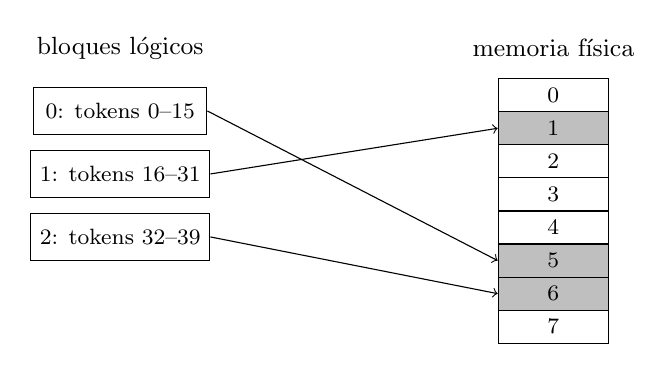
\begin{tikzpicture}[font=\footnotesize,
  lb/.style={draw,minimum width=2.2cm,minimum height=6mm},
  pb/.style={draw,minimum width=1.4cm,minimum height=4.2mm,inner sep=1pt}]
  \node[font=\small] at (0,1.0) {bloques lógicos};
  \node[lb] (l0) at (0,0.2) {0: tokens 0--15};
  \node[lb] (l1) at (0,-0.6) {1: tokens 16--31};
  \node[lb] (l2) at (0,-1.4) {2: tokens 32--39};
  \node[font=\small] at (5.5,1.0) {memoria física};
  \foreach \k in {0,...,7} \node[pb] (p\k) at (5.5,0.4-\k*0.42) {\k};
  \foreach \k in {1,5,6} \node[pb,fill=black!25] at (p\k) {\k};
  \draw[->] (l0.east) -- (p5.west);
  \draw[->] (l1.east) -- (p1.west);
  \draw[->] (l2.east) -- (p6.west);
\end{tikzpicture}
\caption{Una secuencia de 40 tokens con bloques de 16. La tabla de bloques ($0\mapsto 5$, $1\mapsto 1$, $2\mapsto 6$) la sitúa en tres bloques físicos no contiguos; solo se desperdician 8 posiciones del último bloque.}
\label{fig:paged}
\end{figure}

\begin{proposicion}[Desperdicio acotado]\label{prop:desperdicio}
Con bloques de $b_{\mathrm{blk}}$ tokens, una secuencia de $\ell\ge 1$ tokens ocupa $\lceil\ell/b_{\mathrm{blk}}\rceil$ bloques y desperdicia $b_{\mathrm{blk}}\lceil\ell/b_{\mathrm{blk}}\rceil-\ell\le b_{\mathrm{blk}}-1$ posiciones. Como todos los bloques tienen el mismo tamaño, no hay fragmentación externa: cualquier bloque libre sirve a cualquier secuencia.
\end{proposicion}

\begin{proof}
Por la definición de la parte entera superior, $b_{\mathrm{blk}}\lceil\ell/b_{\mathrm{blk}}\rceil$ es el menor múltiplo de $b_{\mathrm{blk}}$ mayor o igual que $\ell$, y su diferencia con $\ell$ es menor que $b_{\mathrm{blk}}$. Un bloque libre puede asignarse a cualquier entrada de cualquier tabla, porque la traducción no exige contigüidad.
\end{proof}

\begin{ejemplo}\label{ej:bloques}
Una respuesta de $300$ tokens con bloques de $16$ ocupa $\lceil 300/16\rceil=19$ bloques, $304$ posiciones, y desperdicia $4$. Con una reserva contigua de $2048$ posiciones desperdiciaría $1748$, el $85{,}4\,\%$. El tamaño de bloque por defecto de vLLM es $16$: bloques más pequeños desperdician menos, pero reducen el paralelismo de la lectura de la caché~\cite[§7.2]{kwon}.
\end{ejemplo}

\begin{proposicion}[Compartición de prefijos]\label{prop:prefijo}
Sean $n_s$ secuencias que comparten un prompt de $P$ tokens. Con compartición de bloques y \emph{copia en escritura}, el prompt ocupa $\lfloor P/b_{\mathrm{blk}}\rfloor$ bloques completos compartidos más, si $P$ no es múltiplo de $b_{\mathrm{blk}}$, una copia del bloque parcial por secuencia, en lugar de $n_s\lceil P/b_{\mathrm{blk}}\rceil$ bloques.
\end{proposicion}

\begin{proof}
Los bloques completos del prompt no se modifican nunca y pueden apuntarse desde las $n_s$ tablas, con un contador de referencias. El último bloque, si está incompleto, recibirá tokens distintos en cada secuencia; al primer intento de escritura se copia (copia en escritura), de modo que acaba habiendo una copia por secuencia~\cite[§4.3 y §4.4]{kwon}.
\end{proof}

Este mecanismo sirve para el muestreo de varias respuestas por prompt, para la búsqueda en haz y para los prompts de sistema comunes. Las API públicas de Anthropic y de Google ofrecen una caché de prefijos del prompt (\emph{prompt caching} y \emph{context caching}) como función documentada; su implementación interna no es pública.

\begin{lecturas}
\item CS336~\cite{cs336}, clase~10 «Inference»: \emph{throughput and latency}, \emph{continuous batching} y \emph{paged attention}.
\item Yu \emph{et al.}~\cite{orca}, planificación por iteración y \emph{batching} selectivo.
\item Kwon \emph{et al.}~\cite{kwon}, secciones~3 («Memory Challenges in LLM Serving») y~4 («Method»), y §7.2.
\item Pope \emph{et al.}~\cite{pope}, sección~2 «Inference Cost Tradeoffs».
\end{lecturas}

\section*{Ejercicios del tema 6}
\addcontentsline{toc}{section}{Ejercicios del tema 6}

\begin{ejercicio}{1}{eje:6-paginacion}
Explique con la analogía de la memoria virtual de un sistema operativo qué problemas resuelve PagedAttention y qué papel tiene la tabla de bloques. ¿Qué equivale a compartir una página de solo lectura entre procesos?
\end{ejercicio}

\begin{ejercicio}{2}{eje:6-bloques}
Una petición con $1000$ tokens de caché se guarda en bloques de $16$. ¿Cuántos bloques ocupa y cuántas posiciones desperdicia? Compárelo con una reserva contigua de $2048$ posiciones.
\end{ejercicio}

\begin{ejercicio}{2}{eje:6-latencia}
(a) Un modelo de $1{,}3\cdot 10^{10}$ parámetros en fp16 se sirve con lote~1 en un acelerador de $300$~TFLOP/s, aprovechado al $50\,\%$ en el \emph{prefill}, y $1$~TB/s. Para un prompt de $2000$ tokens y una respuesta de $500$, estime el $\TTFT$ (sin cola), el $\TPOT$ y la latencia total. (b) Un lote estático de 4 peticiones tiene respuestas de $100$, $400$, $250$ y $50$ tokens. Calcule su utilización.
\end{ejercicio}

\begin{ejercicio}{2}{eje:6-gqa}
Continúe el \cref{eje:2-llama13}. Con GQA de $8$ cabezas de clave y valor, los parámetros bajan a $1{,}1338\cdot 10^{10}$ (las proyecciones de clave y valor se reducen). Con los mismos supuestos, calcule la caché por secuencia y, para $B=64$ y $B=256$, la memoria total, la latencia y el rendimiento. ¿Caben en 80~GB? Compare con la atención multicabeza.
\fuente{adaptado de CS336~\cite{cs336}, clase~10 «Inference», apartado \emph{reduce KV cache size} (GQA en Llama~2 13B).}
\end{ejercicio}

\begin{ejercicio}{2}{eje:6-prefijo}
Cuatro muestras de una misma petición comparten un prompt de $1000$ tokens, con bloques de $16$ y la caché de Llama~2 7B ($512$~KiB por token). Calcule los bloques del prompt sin y con compartición y la memoria ahorrada.
\end{ejercicio}

\begin{ejercicio}{3}{eje:6-frag}
(a) Suponga que la longitud $\ell$ de las secuencias es tal que $\ell\bmod b_{\mathrm{blk}}$ es uniforme en $\{0,\dots,b_{\mathrm{blk}}-1\}$. Demuestre que el desperdicio esperado por secuencia con PagedAttention es $(b_{\mathrm{blk}}-1)/2$. (b) Si las longitudes son uniformes en $\{1,\dots,L_{\max}\}$ y se reservan $L_{\max}$ posiciones contiguas, demuestre que el desperdicio esperado es $(L_{\max}-1)/2$. (c) Calcule ambos para $b_{\mathrm{blk}}=16$ y $L_{\max}=2048$.
\end{ejercicio}


\appendix
% =====================================================================
\chapter{Soluciones de los ejercicios}
\label{ap:soluciones}
% =====================================================================

Cada solución se presenta en cinco partes: datos, planteamiento, desarrollo, resultado y comprobación. En los pasos intermedios se redondea a cuatro cifras significativas salvo que se indique otra cosa. Se usan $e=2{,}718$, $e^{-1}=0{,}3679$, $e^{2}=7{,}389$ y $e^{-2}=0{,}1353$; 1~KiB $=1024$~bytes, 1~MiB $=1024^{2}$~bytes y 1~GiB $=1024^{3}$~bytes, mientras que GB y TB son potencias de~10.

% ---------------------------------------------------------------------
\section{Tema 1}

\begin{solucion}{eje:1-topk-topp}
\datos \emph{top-k} con $k=50$; núcleo con $p=0{,}9$. Caso (a): $p_{(1)}=0{,}95$. Caso (b): 200 tokens de probabilidad $0{,}005$.
\planteamiento \emph{top-k} fija el número de tokens; el núcleo fija la masa conservada (\cref{prop:nucleo}) y, por la \cref{prop:tv-truncada}, la masa eliminada es la distorsión.
\pasos
\begin{enumerate}[label=\arabic*.]
  \item (a) Núcleo: la acumulada del primer token es $0{,}95\ge 0{,}9$; se conserva \textbf{1} token y se elimina una masa $0{,}05$.
  \item (a) \emph{Top-k}: se conservan 50 tokens; los 49 últimos se reparten como mucho la masa $0{,}05$ y son cola de baja calidad.
  \item (b) Núcleo: hace falta $k^{\ast}$ con $0{,}005\,k^{\ast}\ge 0{,}9$, es decir, $k^{\ast}=0{,}9/0{,}005=180$ tokens; se elimina $1-0{,}9=0{,}1$.
  \item (b) \emph{Top-k}: los 50 tokens conservados suman $50\cdot 0{,}005=0{,}25$; se elimina una masa $0{,}75$ de opciones razonables.
\end{enumerate}
\resultado \textbf{(a) núcleo: 1 token; \emph{top-k}: 50. (b) núcleo: 180 tokens, elimina $0{,}1$; \emph{top-k}: 50 tokens, elimina $0{,}75$.} El núcleo adapta el tamaño del conjunto a la confianza del modelo.
\comprobacion en (b), $\TV=0{,}75$ para \emph{top-k} frente a $\TV=0{,}1\le 1-p$ para el núcleo, como garantiza la \cref{prop:tv-truncada}.
\end{solucion}

\begin{solucion}{eje:1-logits}
\datos $z=(1,0,-1)$ para $A,B,C$.
\planteamiento $p_\tau=\softmax(z/\tau)$ (\cref{def:temperatura}); \emph{top-k} y núcleo según la \cref{def:topk-topp}.
\pasos
\begin{enumerate}[label=\arabic*.]
  \item $\tau=1$: $e^{1}=2{,}718$, $e^{0}=1$, $e^{-1}=0{,}3679$; suma $4{,}086$. $p_1=(0{,}6652;\allowbreak\ 0{,}2447;\allowbreak\ 0{,}0900)$.
  \item $\tau=0{,}5$: $z/\tau=(2,0,-2)$; $7{,}389+1+0{,}1353=8{,}524$. $p_{0{,}5}=(0{,}8668;\allowbreak\ 0{,}1173;\allowbreak\ 0{,}0159)$.
  \item \emph{Top-2}: masa $0{,}6652+0{,}2447=0{,}9100$; distribución $(0{,}6652/0{,}9100;\allowbreak\ 0{,}2447/0{,}9100)=(0{,}7311;\allowbreak\ 0{,}2689)$.
  \item Núcleo $0{,}9$: acumuladas $0{,}6652<0{,}9$ y $0{,}9100\ge 0{,}9$; se conservan $A$ y $B$.
  \item La distribución \emph{top-2} es $e^{z_1}/(e^{z_1}+e^{z_2})=1/(1+e^{-(z_1-z_2)})$, que solo depende de $z_1-z_2=1$: $1/(1+0{,}3679)=0{,}7311$.
\end{enumerate}
\resultado \textbf{$p_1=(0{,}6652;\allowbreak\,0{,}2447;\allowbreak\,0{,}0900)$; $p_{0{,}5}=(0{,}8668;\allowbreak\,0{,}1173;\allowbreak\,0{,}0159)$; \emph{top-2}: $(0{,}7311;\allowbreak\,0{,}2689)$; el núcleo $0{,}9$ conserva $A$ y $B$.}
\comprobacion $0{,}6652+0{,}2447+0{,}0900=0{,}9999\approx 1$ y $0{,}8668+0{,}1173+0{,}0159=1$.
\end{solucion}

\begin{solucion}{eje:1-slp}
\datos $u=(1{,}2;\allowbreak\ 0{,}9;\allowbreak\ 0{,}1;\allowbreak\ -0{,}5)$; $\tau\in\{1;\allowbreak\ 0{,}2;\allowbreak\ 2\}$.
\planteamiento $p_\tau(i)=e^{u_i/\tau}/\sum_j e^{u_j/\tau}$ y la \cref{prop:limites-tau}.
\pasos
\begin{enumerate}[label=\arabic*.]
  \item $\tau=1$: $e^{u}=(3{,}320;\allowbreak\ 2{,}460;\allowbreak\ 1{,}105;\allowbreak\ 0{,}6065)$, suma $7{,}491$; $p_1=(0{,}4432;\allowbreak\ 0{,}3283;\allowbreak\ 0{,}1475;\allowbreak\ 0{,}0810)$.
  \item $\tau=0{,}2$: $u/\tau=(6;\allowbreak\ 4{,}5;\allowbreak\ 0{,}5;\allowbreak\ -2{,}5)$; $e^{u/\tau}=(403{,}4;\allowbreak\ 90{,}02;\allowbreak\ 1{,}649;\allowbreak\ 0{,}0821)$, suma $495{,}2$; $p_{0{,}2}=(0{,}8147;\allowbreak\ 0{,}1818;\allowbreak\ 0{,}0033;\allowbreak\ 0{,}0002)$.
  \item $\tau=2$: $u/\tau=(0{,}6;\allowbreak\ 0{,}45;\allowbreak\ 0{,}05;\allowbreak\ -0{,}25)$; $e^{u/\tau}=(1{,}822;\allowbreak\ 1{,}568;\allowbreak\ 1{,}051;\allowbreak\ 0{,}7788)$, suma $5{,}221$; $p_2=(0{,}3490;\allowbreak\ 0{,}3004;\allowbreak\ 0{,}2014;\allowbreak\ 0{,}1492)$.
  \item Sumas: $0{,}4432+0{,}3283+0{,}1475+0{,}0810=1{,}0000$; $0{,}8147+0{,}1818+0{,}0033+0{,}0002=1{,}0000$; $0{,}3490+0{,}3004+0{,}2014+0{,}1492=1{,}0000$.
  \item (b) El máximo $1{,}2$ es único: por la \cref{prop:limites-tau}, $p_\tau\to(1,0,0,0)$ si $\tau\to 0$ (búsqueda voraz) y $p_\tau\to(\frac14,\frac14,\frac14,\frac14)$ si $\tau\to\infty$.
\end{enumerate}
\resultado \textbf{$p_1=(0{,}4432;\allowbreak\,0{,}3283;\allowbreak\,0{,}1475;\allowbreak\,0{,}0810)$, $p_{0{,}2}=(0{,}8147;\allowbreak\,0{,}1818;\allowbreak\,0{,}0033;\allowbreak\,0{,}0002)$, $p_2=(0{,}3490;\allowbreak\,0{,}3004;\allowbreak\,0{,}2014;\allowbreak\,0{,}1492)$; voraz si $\tau\to 0$, uniforme si $\tau\to\infty$.}
\comprobacion la tendencia es la esperada: la probabilidad del primer token crece al bajar $\tau$ ($0{,}3490<0{,}4432<0{,}8147$), y $p_1$ coincide con los valores $0{,}44$, $0{,}33$, $0{,}15$ y $0{,}08$ de la figura~7.17 de~\cite{jm3}.
\end{solucion}

\begin{solucion}{eje:1-nucleo}
\datos $v=(1;\allowbreak\ 0{,}5;\allowbreak\ 0;\allowbreak\ -1)$; $\tau\in\{1;\allowbreak\ 0{,}5\}$; $p=0{,}8$.
\planteamiento softmax con temperatura y, después, núcleo: ordenar, acumular y cortar en cuanto la suma llega a $0{,}8$.
\pasos
\begin{enumerate}[label=\arabic*.]
  \item $\tau=1$: $e^{v}=(2{,}718;\allowbreak\ 1{,}649;\allowbreak\ 1;\allowbreak\ 0{,}3679)$, suma $5{,}735$; $p_1=(0{,}4740;\allowbreak\ 0{,}2875;\allowbreak\ 0{,}1744;\allowbreak\ 0{,}0641)$.
  \item Acumuladas: $0{,}4740$; $0{,}7615$; $0{,}9359$. Se conservan tres tokens; renormalizando por $0{,}9359$: $(0{,}5065;\allowbreak\ 0{,}3072;\allowbreak\ 0{,}1863;\allowbreak\ 0)$.
  \item $\tau=0{,}5$: $v/\tau=(2;\allowbreak\ 1;\allowbreak\ 0;\allowbreak\ -2)$, $e^{v/\tau}=(7{,}389;\allowbreak\ 2{,}718;\allowbreak\ 1;\allowbreak\ 0{,}1353)$, suma $11{,}24$; $p_{0{,}5}=(0{,}6572;\allowbreak\ 0{,}2418;\allowbreak\ 0{,}0889;\allowbreak\ 0{,}0120)$.
  \item Acumuladas: $0{,}6572$; $0{,}8990$. Bastan dos tokens; renormalizando por $0{,}8990$: $(0{,}7311;\allowbreak\ 0{,}2689;\allowbreak\ 0;\allowbreak\ 0)$.
  \item (c) Si $\tau\to 0$, la distribución tiende a $(1,0,0,0)$ (\cref{prop:limites-tau}) y el núcleo conserva un solo token: búsqueda voraz.
\end{enumerate}
\resultado \textbf{(a) $p_1=(0{,}4740;\allowbreak\,0{,}2875;\allowbreak\,0{,}1744;\allowbreak\,0{,}0641)$, $p_{0{,}5}=(0{,}6572;\allowbreak\,0{,}2418;\allowbreak\,0{,}0889;\allowbreak\,0{,}0120)$. (b) $\tau=1$: 3 tokens, $(0{,}5065;\allowbreak\,0{,}3072;\allowbreak\,0{,}1863;\allowbreak\,0)$; $\tau=0{,}5$: 2 tokens, $(0{,}7311;\allowbreak\,0{,}2689;\allowbreak\,0;\allowbreak\,0)$. (c) Voraz.}
\comprobacion con $\tau=0{,}5$ la diferencia entre los dos primeros logits escalados es $2-1=1$ y $1/(1+e^{-1})=0{,}7311$.
\end{solucion}

\begin{solucion}{eje:1-haz}
\datos $K=50\,000$, $T=20$, $m=4$; candidatas $(L=3,\ P=0{,}12)$ y $(L=5,\ P=0{,}08)$; $a=0{,}75$.
\planteamiento la voraz evalúa $K$ extensiones por paso y el haz $mK$ (\cref{prop:coste-haz}); la exhaustiva, $K^{T}$ (\cref{prop:exhaustiva}). Puntuación de la \cref{obs:longitud}.
\pasos
\begin{enumerate}[label=\arabic*.]
  \item Voraz: $KT=50\,000\cdot 20=10^{6}$.
  \item Haz: $mKT=4\cdot 10^{6}$.
  \item Exhaustiva: $\log_{10}K^{T}=20\cdot 4{,}699=93{,}98$, luego $K^{T}\approx 9{,}537\cdot 10^{93}$.
  \item Candidata 1: $\ln 0{,}12=-2{,}120$; $3^{0{,}75}=e^{0{,}75\cdot 1{,}099}=e^{0{,}8240}=2{,}280$; puntuación $-2{,}120/2{,}280=-0{,}9301$.
  \item Candidata 2: $\ln 0{,}08=-2{,}526$; $5^{0{,}75}=e^{0{,}75\cdot 1{,}609}=e^{1{,}207}=3{,}344$; puntuación $-2{,}526/3{,}344=-0{,}7554$.
  \item Con normalización gana la 2 ($-0{,}7554>-0{,}9301$); sin ella gana la 1 ($-2{,}120>-2{,}526$).
  \item (c) Sí: con $m\ge K^{T-1}$ el haz no poda y es la búsqueda exhaustiva; con $m=1$ es la voraz (\cref{prop:coste-haz}).
\end{enumerate}
\resultado \textbf{(a) $10^{6}$, $4\cdot 10^{6}$ y $\approx 9{,}537\cdot 10^{93}$ evaluaciones. (b) Con $a=0{,}75$ gana la candidata larga; sin normalizar, la corta. (c) Sí, con un haz que no poda.}
\comprobacion sin normalización cada token añade un logaritmo negativo y las secuencias largas siempre salen perjudicadas, como indica la \cref{obs:longitud}.
\end{solucion}

\begin{solucion}{eje:1-potencia}
\datos $P=(0{,}6;\allowbreak\ 0{,}3;\allowbreak\ 0{,}1)$; $Q\propto P^{a}$.
\planteamiento por la \cref{prop:potencia}, $Q$ es la distribución con temperatura $\tau=1/a$.
\pasos
\begin{enumerate}[label=\arabic*.]
  \item (a) Duplicar la temperatura: $\tau=2$, $a=\frac12$. Reducirla a la mitad: $\tau=\frac12$, $a=2$.
  \item $a=2$: $P^{2}=(0{,}36;\allowbreak\ 0{,}09;\allowbreak\ 0{,}01)$, suma $0{,}46$; $Q=(0{,}7826;\allowbreak\ 0{,}1957;\allowbreak\ 0{,}0217)$.
  \item $a=\frac12$: $\sqrt P=(0{,}7746;\allowbreak\ 0{,}5477;\allowbreak\ 0{,}3162)$, suma $1{,}639$; $Q=(0{,}4727;\allowbreak\ 0{,}3343;\allowbreak\ 0{,}1930)$.
  \item (c) $\tau\to 0$ equivale a $a\to\infty$: domina el mayor $P(i)$ y $Q\to(1,0,0)$. $\tau\to\infty$ equivale a $a\to 0$: $P(i)^{0}=1$ y $Q\to(\frac13,\frac13,\frac13)$.
\end{enumerate}
\resultado \textbf{(a) $a=\frac12$ duplica $\tau$ y $a=2$ la reduce a la mitad. (b) $a=2$: $(0{,}7826;\allowbreak\,0{,}1957;\allowbreak\,0{,}0217)$; $a=\frac12$: $(0{,}4727;\allowbreak\,0{,}3343;\allowbreak\,0{,}1930)$. (c) Voraz y uniforme.}
\comprobacion las dos distribuciones suman~1; con $a=2$ se afila ($0{,}6\to 0{,}7826$) y con $a=\frac12$ se aplana ($0{,}6\to 0{,}4727$).
\end{solucion}

\begin{solucion}{eje:1-entropia}
\datos $p_\tau(i)=e^{z_i/\tau}/Z(\tau)$ con $Z(\tau)=\sum_je^{z_j/\tau}$; en (c), $z=(1,0,-1)$ y $\tau=1$.
\planteamiento se trabaja con $\beta=1/\tau$ y se aplica la regla de la cadena, $\frac{\mathrm{d}H}{\mathrm{d}\tau}=\frac{\mathrm{d}H}{\mathrm{d}\beta}\,\frac{\mathrm{d}\beta}{\mathrm{d}\tau}$.
\pasos
\begin{enumerate}[label=\arabic*.]
  \item Con $\beta=1/\tau$, $\ln p_\tau(i)=\beta z_i-\ln Z$ y $H=-\sum_ip_\tau(i)(\beta z_i-\ln Z)=\ln Z-\beta\,\E[z]$, donde $\E[z]=\sum_i p_\tau(i)z_i$.
  \item $\dfrac{\mathrm{d}\ln Z}{\mathrm{d}\beta}=\dfrac{\sum_jz_je^{\beta z_j}}{Z}=\E[z]$.
  \item $\dfrac{\mathrm{d}\E[z]}{\mathrm{d}\beta}=\sum_iz_i\,p_\tau(i)\bigl(z_i-\E[z]\bigr)=\E[z^{2}]-\E[z]^{2}=\Var_{p_\tau}(z)$, usando $\frac{\mathrm{d}p_\tau(i)}{\mathrm{d}\beta}=p_\tau(i)(z_i-\E[z])$.
  \item $\dfrac{\mathrm{d}H}{\mathrm{d}\beta}=\E[z]-\E[z]-\beta\Var(z)=-\beta\Var(z)$.
  \item $\dfrac{\mathrm{d}\beta}{\mathrm{d}\tau}=-\dfrac{1}{\tau^{2}}$, luego $\dfrac{\mathrm{d}H}{\mathrm{d}\tau}=\beta\Var(z)\dfrac{1}{\tau^{2}}=\dfrac{\Var(z)}{\tau^{3}}\ge 0$.
  \item (b) Como $p_\tau(i)>0$ para todo $i$, $\Var_{p_\tau}(z)=0$ si y solo si todos los $z_i$ son iguales; entonces $p_\tau$ es uniforme para todo $\tau$ y $H=\ln K$ es constante.
  \item (c) $p_1=(0{,}6652;\allowbreak\ 0{,}2447;\allowbreak\ 0{,}0900)$; $\E[z]=0{,}6652-0{,}0900=0{,}5752$; $\E[z^{2}]=0{,}6652+0{,}0900=0{,}7553$; $\Var(z)=0{,}7553-0{,}5752^{2}=0{,}7553-0{,}3309=0{,}4244$.
\end{enumerate}
\resultado \textbf{$\mathrm{d}H/\mathrm{d}\tau=\Var_{p_\tau}(z)/\tau^{3}\ge 0$; es nula solo si todos los logits son iguales; en el caso (c) vale $0{,}4244$.} \hfill$\blacksquare$
\comprobacion una diferencia centrada, $(H(1{,}001)-H(0{,}999))/0{,}002$, da $0{,}4244$; además, los valores del \cref{ej:muestreo} cumplen $H(0{,}5)=0{,}455<H(1)=0{,}948<H(2)=1{,}245$ nats.
\end{solucion}

% ---------------------------------------------------------------------
\section{Tema 2}

\begin{solucion}{eje:2-fases}
\datos el mismo Transformer; \emph{prefill} con $n$ tokens a la vez y decodificación con uno por paso.
\planteamiento comparar la intensidad respecto a los pesos con la intensidad crítica $\Icrit$ (\cref{prop:intensidad-capas}).
\pasos
\begin{enumerate}[label=\arabic*.]
  \item \emph{Prefill}: cada peso de 2 bytes se lee una vez y se usa con los $n$ tokens, a 2 FLOP por token: $2n/2=n$ FLOP/byte.
  \item Decodificación: cada peso se usa con un solo token: $2/2=1$ FLOP/byte.
  \item Con $\Icrit=150$ (\cref{ej:cota}), un prompt de $n=1000$ tokens supera la intensidad crítica y queda limitado por el cómputo; la decodificación, con $1\ll 150$, por la memoria.
\end{enumerate}
\resultado \textbf{el \emph{prefill} reutiliza cada peso $n$ veces y queda limitado por el cómputo; la decodificación lo usa una vez y queda limitada por el ancho de banda.}
\comprobacion un prompt de un solo token tendría la misma intensidad que un paso de decodificación: las dos fases solo se distinguen por cuántos tokens comparten cada lectura de pesos.
\end{solucion}

\begin{solucion}{eje:2-vf}
\planteamiento contrastar con el \cref{teo:cache}, la \cref{prop:lote} y la \cref{prop:tam-cache}.
\pasos
\begin{enumerate}[label=(\alph*)]
  \item \textbf{Falsa.} Por el \cref{teo:cache}, la caché guarda exactamente lo que se recalcularía; solo cambia el coste (salvo diferencias de redondeo en coma flotante).
  \item \textbf{Falsa.} Por la \cref{prop:lote}, $R(B)=B/(t_0+Bt_1)$ crece menos que linealmente; en la \cref{tab:lote}, pasar de $B=32$ a $B=64$ lleva el rendimiento de $1346$ a $1578$ tokens/s, un factor $1{,}17$.
  \item \textbf{Verdadera.} La caché es proporcional a $\nkv$, que se divide por $32/8=4$; en la misma memoria caben cuatro veces más secuencias de la misma longitud.
\end{enumerate}
\resultado \textbf{(a) falsa; (b) falsa; (c) verdadera.}
\end{solucion}

\begin{solucion}{eje:2-kv}
\datos $L=24$, $\nkv=16$, $\dhd=64$, $s=2$; $S=2048$; $B=16$.
\planteamiento \cref{prop:tam-cache}: $c_{\mathrm{kv}}=2L\nkv\dhd s$; se multiplica por tokens y por secuencias.
\pasos
\begin{enumerate}[label=\arabic*.]
  \item $c_{\mathrm{kv}}=2\cdot 24\cdot 16\cdot 64\cdot 2=98\,304$~bytes; $98\,304/1024=96$~KiB.
  \item Por secuencia: $96\cdot 2048=196\,608$~KiB $=196\,608/1024=192$~MiB.
  \item Lote: $192\cdot 16=3072$~MiB $=3$~GiB.
\end{enumerate}
\resultado \textbf{96~KiB por token, 192~MiB por secuencia y 3~GiB para el lote.}
\comprobacion $98\,304\cdot 2048\cdot 16=3\,221\,225\,472$~bytes $=3\cdot 1024^{3}$.
\end{solucion}

\begin{solucion}{eje:2-cota}
\datos $N=1{,}3\cdot 10^{10}$; $\Bmem=10^{12}$~bytes/s; $s\in\{2;\allowbreak\,1;\allowbreak\,0{,}5\}$.
\planteamiento \cref{teo:cota-memoria} con $B=1$: $\text{tokens/s}\le\Bmem/(sN)$.
\pasos
\begin{enumerate}[label=\arabic*.]
  \item fp16: $sN=2{,}6\cdot 10^{10}$~bytes; cota $10^{12}/2{,}6\cdot 10^{10}=38{,}46$ tokens/s.
  \item int8: $sN=1{,}3\cdot 10^{10}$~bytes; cota $76{,}92$ tokens/s.
  \item int4: $sN=6{,}5\cdot 10^{9}$~bytes; cota $153{,}8$ tokens/s.
\end{enumerate}
\resultado \textbf{$38{,}46$, $76{,}92$ y $153{,}8$ tokens/s.}
\comprobacion $153{,}8/38{,}46=4{,}0=2/0{,}5$, el cociente de bytes por peso.
\end{solucion}

\begin{solucion}{eje:2-llama13}
\datos $N=1{,}3015\cdot 10^{10}$; bf16 ($s=2$); $L=40$, $\nkv=40$, $\dhd=128$; $S=1024$; $\Bmem=3{,}35\cdot 10^{12}$~bytes/s; memoria de 80~GB.
\planteamiento memoria $=sN+B\,S\,c_{\mathrm{kv}}$; latencia por paso $=$ memoria$/\Bmem$ (\cref{teo:cota-memoria}); rendimiento $=B/$latencia.
\pasos
\begin{enumerate}[label=\arabic*.]
  \item $c_{\mathrm{kv}}=2\cdot 40\cdot 40\cdot 128\cdot 2=819\,200$~bytes; por secuencia, $1024\cdot 819\,200=8{,}389\cdot 10^{8}$~bytes $=0{,}8389$~GB.
  \item Pesos: $2\cdot 1{,}3015\cdot 10^{10}=26{,}03$~GB.
  \item $B=1$: memoria $26{,}03+0{,}84=26{,}87$~GB; latencia $26{,}87\cdot 10^{9}/3{,}35\cdot 10^{12}=8{,}02$~ms; rendimiento $1/0{,}00802=124{,}7$ tokens/s.
  \item $B=64$: caché $64\cdot 0{,}8389=53{,}69$~GB; memoria $79{,}72$~GB; latencia $23{,}80$~ms; rendimiento $64/0{,}02380=2689$ tokens/s.
  \item $B=256$: caché $214{,}7$~GB; memoria $240{,}8$~GB; latencia $71{,}87$~ms; rendimiento $256/0{,}07187=3562$ tokens/s.
  \item (c) $B=1$ y $B=64$ caben en 80~GB (este último por muy poco); $B=256$ no.
\end{enumerate}
\resultado \textbf{caché de $0{,}839$~GB por secuencia; $(B,\text{memoria},\text{latencia},\text{rendimiento})=(1;\allowbreak\ 26{,}87~\text{GB};\allowbreak\ 8{,}02~\text{ms};\allowbreak\ 124{,}7)$, $(64;\allowbreak\ 79{,}72;\allowbreak\ 23{,}80;\allowbreak\ 2689)$, $(256;\allowbreak\ 240{,}8;\allowbreak\ 71{,}87;\allowbreak\ 3562)$.} Aumentar el lote empeora la latencia y mejora el rendimiento con rendimientos decrecientes; con $B=256$ la caché no cabe en la GPU.
\comprobacion el límite de la \cref{prop:lote} es $\Bmem/(S\,c_{\mathrm{kv}})=3{,}35\cdot 10^{12}/8{,}389\cdot 10^{8}=3993$ tokens/s, por encima de los tres valores y cada vez más próximo.
\end{solucion}

\begin{solucion}{eje:2-intensidad}
\datos lote $B$; pesos en fp16 (2 bytes); $\Icrit=150$~FLOP/byte.
\planteamiento contar, para un peso, las operaciones y los bytes en un paso.
\pasos
\begin{enumerate}[label=\arabic*.]
  \item En un paso, cada peso $w$ se lee una vez (2 bytes) y participa en una multiplicación y una suma por cada una de las $B$ secuencias: $2B$ FLOP.
  \item Intensidad respecto a los pesos: $2B/2=B$ FLOP/byte. \hfill$\blacksquare$
  \item Deja de estar limitado por los pesos si $B\ge\Icrit=150$.
  \item La caché KV es distinta para cada secuencia: cada número de la caché se lee en cada paso y se usa con una sola consulta, con intensidad menor que~1 (\cref{prop:intensidad-capas}(b)).
  \item Su tamaño crece con $B$: con Llama~2 7B y 2000 tokens, para $B=64$ ya son $67{,}1$~GB frente a $14$~GB de pesos (\cref{tab:lote}), y puede no caber en la memoria.
\end{enumerate}
\resultado \textbf{la intensidad es $B$ FLOP/byte; harían falta unas 150 secuencias por lote, pero la caché, con intensidad menor que~1 y tamaño proporcional a $B$, domina antes el tráfico y la memoria.}
\comprobacion con $B=1$ se recupera la intensidad de $1$~FLOP/byte del \cref{ej:cota}.
\end{solucion}

\begin{solucion}{eje:2-sincache}
\datos una capa de atención de dimensión $D$; prompt vacío; $T$ tokens generados.
\planteamiento el producto de $a$ consultas por $b$ claves cuesta $2abD$ FLOP, y el de los pesos de atención por los valores, otros $2abD$ (\cref{prop:intensidad-capas}).
\pasos
\begin{enumerate}[label=\arabic*.]
  \item Sin caché, el paso $t$ recalcula la atención completa sobre $t$ posiciones: $a=b=t$, coste $4Dt^{2}$.
  \item Total: $\sum_{t=1}^{T}4Dt^{2}=4D\frac{T(T+1)(2T+1)}{6}=\frac23DT(T+1)(2T+1)=\Theta(T^{3})$.
  \item Con caché, el paso $t$ calcula una consulta frente a $t$ claves: $a=1$, $b=t$, coste $4Dt$.
  \item Total: $\sum_{t=1}^{T}4Dt=4D\frac{T(T+1)}{2}=2DT(T+1)=\Theta(T^{2})$. \hfill$\blacksquare$
  \item Cociente: $\frac{\frac23DT(T+1)(2T+1)}{2DT(T+1)}=\frac{2T+1}{3}$; con $T=1000$, $2001/3=667$.
\end{enumerate}
\resultado \textbf{$\Theta(T^{3})$ sin caché frente a $\Theta(T^{2})$ con caché; para $T=1000$ la caché reduce el coste de la atención unas 667 veces.}
\comprobacion para $T=1$ ambos costes valen $4D$ y el cociente es $3/3=1$, como debe ser: con un solo token no hay nada que reutilizar.
\end{solucion}

% ---------------------------------------------------------------------
\section{Tema 3}

\begin{solucion}{eje:3-vf}
\planteamiento contrastar con los \cref{teo:especulativa,teo:especulativa-secuencias} y la \cref{def:ronda}.
\pasos
\begin{enumerate}[label=(\alph*)]
  \item \textbf{Falsa.} Por el \cref{teo:especulativa-secuencias}, la salida tiene exactamente la distribución del objetivo; solo cambia el tiempo.
  \item \textbf{Verdadera.} Si $q=p$, $\min(1,p/q)=1$ para todo token y $\beta=1$ (\cref{lem:residuo}).
  \item \textbf{Verdadera.} Si se rechaza la primera propuesta se emite un token del residuo; si no, al menos esa propuesta. Si se aceptan todas se emiten $\gamma+1$.
\end{enumerate}
\resultado \textbf{(a) falsa; (b) verdadera; (c) verdadera.}
\end{solucion}

\begin{solucion}{eje:3-dos}
\datos $p=(0{,}6;\allowbreak\ 0{,}4)$, $q=(0{,}9;\allowbreak\ 0{,}1)$.
\planteamiento aceptación $\min(1,p/q)$; $\beta=\sum\min(p,q)$; residuo $\max(0,p-q)$ normalizado; $P(\text{emitir }x)=\min(p,q)+(1-\beta)r(x)$.
\pasos
\begin{enumerate}[label=\arabic*.]
  \item Aceptar $A$: $\min(1;\allowbreak\ 0{,}6/0{,}9)=2/3\approx 0{,}6667$. Aceptar $B$: $\min(1;\allowbreak\ 0{,}4/0{,}1)=\min(1;4)=1$.
  \item $\beta=\min(0{,}6;0{,}9)+\min(0{,}4;0{,}1)=0{,}6+0{,}1=0{,}7$.
  \item Residuo: $\max(0;-0{,}3)=0$ y $\max(0;0{,}3)=0{,}3$; normalizado, $(0;\allowbreak\ 1)$.
  \item $P(A)=0{,}9\cdot\frac23=0{,}6$; $P(B)=0{,}1\cdot 1+0{,}3\cdot 1=0{,}4$.
\end{enumerate}
\resultado \textbf{aceptación $2/3$ para $A$ y $1$ para $B$; $\beta=0{,}7$; residuo $(0,1)$; salida $(0{,}6;\allowbreak\ 0{,}4)=p$.}
\comprobacion $1-\beta=0{,}3=\frac12(\abs{0{,}6-0{,}9}+\abs{0{,}4-0{,}1})$, como afirma la \cref{prop:beta-tv}.
\end{solucion}

\begin{solucion}{eje:3-cs336}
\datos $\V=\{A,B\}$; $q(A)>p(A)$; en (c), $p=(0{,}3;\allowbreak\ 0{,}7)$ y $q=(0{,}8;\allowbreak\ 0{,}2)$.
\planteamiento se aplica la regla de aceptación y rechazo token a token.
\pasos
\begin{enumerate}[label=\arabic*.]
  \item (a) $q(B)=1-q(A)<1-p(A)=p(B)$. Residuo: $\max(0,p(A)-q(A))=0$ y $\max(0,p(B)-q(B))=p(B)-q(B)>0$; normalizado, $(0,1)$.
  \item (b) Se propone $A$ con probabilidad $q(A)$ y se acepta con $p(A)/q(A)<1$: $P(\text{emitir }A)=q(A)\cdot\frac{p(A)}{q(A)}+0=p(A)$, porque el residuo nunca da $A$.
  \item Se emite $B$ si se propone y se acepta (probabilidad $q(B)\cdot 1$) o si se propone $A$, se rechaza y el residuo da $B$ (probabilidad $q(A)\bigl(1-\frac{p(A)}{q(A)}\bigr)\cdot 1=q(A)-p(A)$).
  \item $P(\text{emitir }B)=q(B)+q(A)-p(A)=1-p(A)=p(B)$.
  \item (c) Aceptar $A$: $0{,}3/0{,}8=0{,}375$; $P(A)=0{,}8\cdot 0{,}375=0{,}3$; $P(B)=0{,}2+0{,}8-0{,}3=0{,}7$.
\end{enumerate}
\resultado \textbf{$P(\text{emitir }A)=p(A)$ y $P(\text{emitir }B)=p(B)$; en (c), $(0{,}3;\allowbreak\ 0{,}7)$.}
\comprobacion $\beta=\min(0{,}3;0{,}8)+\min(0{,}7;0{,}2)=0{,}5$ y $\TV(p,q)=\frac12(0{,}5+0{,}5)=0{,}5=1-\beta$.
\end{solucion}

\begin{solucion}{eje:3-gamma}
\datos $\alpha=0{,}5$; $\gamma\in\{2,3,10\}$; $c=0{,}1$.
\planteamiento $\E[N_{\mathrm{r}}]=(1-\alpha^{\gamma+1})/(1-\alpha)$ (\cref{teo:tokens-ronda}) y $f(\gamma)=\E[N_{\mathrm{r}}]/(\gamma c+1)$ (\cref{teo:mejora}).
\pasos
\begin{enumerate}[label=\arabic*.]
  \item $\gamma=3$: $0{,}5^{4}=0{,}0625$; $\E[N_{\mathrm{r}}]=0{,}9375/0{,}5=1{,}875$.
  \item $\gamma=10$: $0{,}5^{11}=0{,}000488$; $\E[N_{\mathrm{r}}]=0{,}9995/0{,}5=1{,}999$.
  \item $\gamma=2$: $0{,}5^{3}=0{,}125$; $\E[N_{\mathrm{r}}]=0{,}875/0{,}5=1{,}75$.
  \item Factores: $f(2)=1{,}75/1{,}2=1{,}458$; $f(3)=1{,}875/1{,}3=1{,}442$; $f(10)=1{,}999/2=0{,}9995$.
\end{enumerate}
\resultado \textbf{$1{,}875$ y $1{,}999$ tokens por ronda; $f(2)=1{,}458$, $f(3)=1{,}442$ y $f(10)=0{,}9995$.} Con $\gamma=10$ se ganan $0{,}124$ tokens por ronda a cambio de 7 pasadas del borrador, y el resultado es más lento que no especular. Con $\alpha$ bajo conviene $\gamma$ pequeño; aquí el óptimo es $\gamma=2$.
\comprobacion el límite de $\E[N_{\mathrm{r}}]$ es $1/(1-\alpha)=2$, y con $\gamma=3$ ya se tiene el $93{,}75\,\%$ de ese máximo.
\end{solucion}

\begin{solucion}{eje:3-tv}
\datos $\tilde x\sim q$; $\beta=\sum_x\min(p(x),q(x))$; $p$ y $q$ son distribuciones.
\planteamiento (a) sin rechazo la salida es la propuesta; (b) escribir $1-\beta$ como suma de partes positivas.
\pasos
\begin{enumerate}[label=\arabic*.]
  \item (a) Si se acepta siempre, el token emitido es $\tilde x$, y $P(\text{emitir }x)=q(x)$, que solo coincide con $p$ si $p=q$.
  \item (b) Por el \cref{lem:residuo}, $1-\beta=\sum_x\max(0,p(x)-q(x))$.
  \item Como $\sum_x(p-q)=1-1=0$, las partes positiva y negativa suman lo mismo: $\sum_x\max(0,p-q)=\sum_x\max(0,q-p)$.
  \item Para cada $x$, $\abs{p-q}=\max(0,p-q)+\max(0,q-p)$; sumando, $\sum_x\abs{p-q}=2\sum_x\max(0,p-q)$.
  \item Luego $1-\beta=\frac12\sum_x\abs{p(x)-q(x)}=\TV(p,q)$. \hfill$\blacksquare$
\end{enumerate}
\resultado \textbf{sin rechazo la salida sigue $q$; la probabilidad de rechazo es $1-\beta=\TV(p,q)$.}
\comprobacion en el \cref{ej:especulativa}, $\frac12(0{,}3+0{,}3+0)=0{,}3=1-0{,}7$.
\end{solucion}

\begin{solucion}{eje:3-optimo}
\datos $0<\alpha<1$, $c>0$; $\E[N_{\mathrm{r}}](\gamma)=\sum_{j=0}^{\gamma}\alpha^{j}$; $f(\gamma)=\E[N_{\mathrm{r}}](\gamma)/(\gamma c+1)$.
\planteamiento acotar la suma geométrica y estudiar el cociente.
\pasos
\begin{enumerate}[label=\arabic*.]
  \item (a) $\E[N_{\mathrm{r}}](\gamma+1)-\E[N_{\mathrm{r}}](\gamma)=\alpha^{\gamma+1}>0$, luego es estrictamente creciente; y $\sum_{j=0}^{\gamma}\alpha^{j}<\sum_{j=0}^{\infty}\alpha^{j}=1/(1-\alpha)$.
  \item (b) $0<f(\gamma)<\dfrac{1}{(1-\alpha)(\gamma c+1)}\to 0$ cuando $\gamma\to\infty$.
  \item Sea $f_1=f(1)>0$. Existe $\gamma_0$ tal que $f(\gamma)<f_1$ para $\gamma>\gamma_0$; el máximo de $f$ sobre $\{1,\dots,\gamma_0\}$, que existe por ser un conjunto finito, es el máximo global.
  \item (c) Como $\alpha^{j}\le\alpha$ para $j\ge 1$, $\E[N_{\mathrm{r}}](\gamma)\le 1+\gamma\alpha\le 1+\gamma c$ si $\alpha\le c$, y entonces $f(\gamma)\le 1$. \hfill$\blacksquare$
\end{enumerate}
\resultado \textbf{$\E[N_{\mathrm{r}}]$ crece estrictamente y está acotado por $1/(1-\alpha)$; $f(\gamma)\to 0$ y hay un $\gamma$ óptimo finito; si $\alpha\le c$, especular nunca compensa.} Junto con el \cref{cor:alpha-c}, la condición $\alpha>c$ es necesaria y suficiente para que exista algún $\gamma$ con $f(\gamma)>1$.
\comprobacion con $\alpha=0{,}5$ y $c=0{,}1$ (\cref{eje:3-gamma}), $f$ vale $1{,}364$; $1{,}458$; $1{,}442$ para $\gamma=1,2,3$ y $0{,}9995$ para $\gamma=10$: sube, alcanza el máximo en $\gamma=2$ y decrece.
\end{solucion}

% ---------------------------------------------------------------------
\section{Tema 4}

\begin{solucion}{eje:4-conceptos}
\planteamiento relacionar cada pregunta con las \cref{def:afin,def:simetrico,def:granularidad} y el \cref{teo:error-cuant}.
\pasos
\begin{enumerate}[label=(\alph*)]
  \item Los pesos se distribuyen de forma aproximadamente simétrica alrededor de~0; el cuantizador simétrico aprovecha bien sus niveles y evita el término de punto cero en el producto (\cref{prop:producto-entero}). Una activación no negativa, como la salida de una ReLU, usaría solo la mitad de los niveles simétricos; el afín coloca los $2^{b}$ niveles en $[0,x_{\max}]$ y reduce el paso a la mitad.
  \item Los ceros son muy frecuentes (relleno, activaciones nulas, pesos podados); si el~0 se representa exactamente, no añaden error ni sesgo.
  \item La escala por canal se adapta al rango de cada canal: un canal de valores pequeños no hereda el paso grande impuesto por otro con valores grandes (\cref{prop:atipico}), y la descuantización sigue siendo un reescalado del producto entero (\cref{prop:factorizar}).
\end{enumerate}
\resultado \textbf{simétrica para pesos centrados y afín para rangos asimétricos; el~0 exacto evita errores en valores muy frecuentes; la escala por canal reduce el error sin romper la aritmética entera.}
\end{solucion}

\begin{solucion}{eje:4-int4}
\datos $x=(-1;\allowbreak\ 0;\allowbreak\ 0{,}62;\allowbreak\ 2)$; $b=4$, enteros $0,\dots,15$.
\planteamiento \cref{def:afin} con calibración por mínimo y máximo.
\pasos
\begin{enumerate}[label=\arabic*.]
  \item $\Delta=(2-(-1))/15=3/15=0{,}2$.
  \item $Z=\rnd(1/0{,}2)=\rnd(5)=5$.
  \item $x/\Delta=(-5;\allowbreak\ 0;\allowbreak\ 3{,}1;\allowbreak\ 10)$; redondeo: $(-5;\allowbreak\ 0;\allowbreak\ 3;\allowbreak\ 10)$.
  \item $Q=(0;\allowbreak\ 5;\allowbreak\ 8;\allowbreak\ 15)$; todos en $[0,15]$, sin recorte.
  \item $\hat x=0{,}2\cdot(-5;\allowbreak\ 0;\allowbreak\ 3;\allowbreak\ 10)=(-1;\allowbreak\ 0;\allowbreak\ 0{,}6;\allowbreak\ 2)$; errores $(0;\allowbreak\ 0;\allowbreak\ 0{,}02;\allowbreak\ 0)$.
  \item $x=3$: $\rnd(3/0{,}2)+5=15+5=20$, recortado a $15$; $\hat x=0{,}2\cdot 10=2$ y el error es $1$.
\end{enumerate}
\resultado \textbf{$\Delta=0{,}2$; $Z=5$; $Q=(0;\allowbreak\,5;\allowbreak\,8;\allowbreak\,15)$; $\hat x=(-1;\allowbreak\,0;\allowbreak\,0{,}6;\allowbreak\,2)$; error máximo $0{,}02$. Con $x=3$ hay saturación y el error es $1$.}
\comprobacion $0{,}02\le\Delta/2=0{,}1$; el~0 se reconstruye exactamente y el error de saturación, $1>0{,}1$, no respeta la cota, como prevé el \cref{teo:error-cuant}.
\end{solucion}

\begin{solucion}{eje:4-3bits}
\datos la matriz $W$; $b=3$, enteros $0,\dots,7$; $x_{\min}=-1{,}6$, $x_{\max}=2{,}6$.
\planteamiento \cref{def:afin} por tensor.
\pasos
\begin{enumerate}[label=\arabic*.]
  \item $\Delta=(2{,}6+1{,}6)/7=4{,}2/7=0{,}6$; $Z=\rnd(1{,}6/0{,}6)=\rnd(2{,}667)=3$.
  \item $W/\Delta$ y su redondeo:
  \[
  \frac{W}{\Delta}=\begin{pmatrix}2 & -0{,}6667 & 0{,}4167\\ -1{,}667 & 4{,}333 & 0\\ 0{,}8333 & -2{,}667 & 3{,}167\end{pmatrix},\qquad
  \rnd\Bigl(\frac{W}{\Delta}\Bigr)=\begin{pmatrix}2 & -1 & 0\\ -2 & 4 & 0\\ 1 & -3 & 3\end{pmatrix}.
  \]
  \item Sumando $Z=3$ (sin recorte) y reconstruyendo con $\hat W=0{,}6\,\rnd(W/\Delta)$:
  \[
  Q=\begin{pmatrix}5 & 2 & 3\\ 1 & 7 & 3\\ 4 & 0 & 6\end{pmatrix},\qquad
  \hat W=\begin{pmatrix}1{,}2 & -0{,}6 & 0\\ -1{,}2 & 2{,}4 & 0\\ 0{,}6 & -1{,}8 & 1{,}8\end{pmatrix}.
  \]
  \item Errores:
  \[
  W-\hat W=\begin{pmatrix}0 & 0{,}2 & 0{,}25\\ 0{,}2 & 0{,}2 & 0\\ -0{,}1 & 0{,}2 & 0{,}1\end{pmatrix}.
  \]
\end{enumerate}
\resultado \textbf{$\Delta=0{,}6$; $Z=3$; error máximo $0{,}25$, en el elemento $0{,}25$, que se reconstruye como~0.}
\comprobacion $0{,}25\le\Delta/2=0{,}3$. El extremo $-1{,}6$ no se reconstruye exactamente ($-1{,}8$) porque $Z$ se redondeó de $2{,}667$ a $3$, pero su error, $0{,}2$, respeta la cota, como garantiza el \cref{teo:error-cuant} también con $Z$ redondeado.
\end{solucion}

\begin{solucion}{eje:4-atipico}
\datos $v=(0{,}12;\allowbreak\,-0{,}31;\allowbreak\,0{,}05;\allowbreak\,0{,}27;\allowbreak\,-0{,}08;\allowbreak\,0{,}19;\allowbreak\,-0{,}22;\allowbreak\,6{,}4)$; int4 simétrico, $\Delta=\max\abs{v}/7$.
\planteamiento \cref{def:simetrico} con distintos grupos.
\pasos
\begin{enumerate}[label=\arabic*.]
  \item (a) Por tensor: $\Delta=6{,}4/7=0{,}9143$. Todos los valores salvo el atípico cumplen $\abs{v_i}<\Delta/2=0{,}457$ y se cuantizan a~0 (\cref{prop:atipico}); el atípico da $Q=7$ y $\hat v=6{,}4$. Error máximo: $0{,}31$.
  \item (b) Grupo 1, $(0{,}12;\allowbreak\,-0{,}31;\allowbreak\,0{,}05;\allowbreak\,0{,}27)$: $\Delta=0{,}31/7=0{,}04429$; $v/\Delta=(2{,}71;\allowbreak\,-7;\allowbreak\,1{,}13;\allowbreak\,6{,}10)$, $Q=(3;\allowbreak\,-7;\allowbreak\,1;\allowbreak\,6)$, $\hat v=(0{,}1329;\allowbreak\,-0{,}31;\allowbreak\,0{,}0443;\allowbreak\,0{,}2657)$; errores $(0{,}0129;\allowbreak\,0;\allowbreak\,0{,}0057;\allowbreak\,0{,}0043)$.
  \item Grupo 2, $(-0{,}08;\allowbreak\,0{,}19;\allowbreak\,-0{,}22;\allowbreak\,6{,}4)$: $\Delta=0{,}9143$; los tres primeros se anulan; errores $(0{,}08;\allowbreak\,0{,}19;\allowbreak\,0{,}22;\allowbreak\,0)$. Error máximo global: $0{,}22$.
  \item (c) Sin el atípico, $\Delta=0{,}31/7=0{,}04429$ para los 7 valores; $Q=(3;\allowbreak\,-7;\allowbreak\,1;\allowbreak\,6;\allowbreak\,-2;\allowbreak\,4;\allowbreak\,-5)$; $\hat v=(0{,}1329;\allowbreak\,-0{,}31;\allowbreak\,0{,}0443;\allowbreak\,0{,}2657;\allowbreak\,-0{,}0886;\allowbreak\,0{,}1771;\allowbreak\,-0{,}2214)$; error máximo $0{,}0129$, y el atípico se guarda exacto en fp16.
\end{enumerate}
\resultado \textbf{errores máximos: $0{,}31$ por tensor, $0{,}22$ por grupos de~4 y $0{,}0129$ separando el atípico.} Los grupos solo ayudan a los que no comparten grupo con el atípico; separarlo, como hace LLM.int8(), resuelve el problema.
\comprobacion en (c), $0{,}0129\le\Delta/2=0{,}0221$; en (a), la cota $\Delta/2=0{,}457$ es $20{,}6$ veces mayor que la de (c), igual que el cociente de escalas $6{,}4/0{,}31=20{,}6$.
\end{solucion}

\begin{solucion}{eje:4-entero}
\datos enteros en $[-127,127]$; acumulador hasta $2^{31}-1=2\,147\,483\,647$; escalas fp16 (16 bits); grupos de $64$ y $128$; $N=7\cdot 10^{9}$.
\planteamiento cada producto vale como mucho $127^{2}$ en módulo; \cref{prop:bits-grupo} para los bits.
\pasos
\begin{enumerate}[label=\arabic*.]
  \item $127^{2}=16\,129$. La suma de $n$ productos cumple $\abs{\sum}\le 16\,129\,n$, que no desborda si $16\,129\,n\le 2\,147\,483\,647$, es decir, $n\le 133\,144{,}25$.
  \item Mayor $n$: $133\,144$.
  \item Grupos de 64: $4+16/64=4{,}25$ bits por peso; memoria $7\cdot 10^{9}\cdot 4{,}25/8=3{,}719\cdot 10^{9}$~bytes.
  \item Grupos de 128: $4+16/128=4{,}125$ bits; memoria $7\cdot 10^{9}\cdot 4{,}125/8=3{,}609\cdot 10^{9}$~bytes.
\end{enumerate}
\resultado \textbf{(a) $n\le 133\,144$. (b) $4{,}25$ bits y $3{,}72$~GB con grupos de 64; $4{,}125$ bits y $3{,}61$~GB con grupos de 128.}
\comprobacion las dimensiones internas de los LLM (unos miles) quedan muy por debajo de $133\,144$, y $3{,}61$~GB coincide con la \cref{tab:formatos}.
\end{solucion}

\begin{solucion}{eje:4-ruido}
\datos $e\sim\mathcal{U}[-\Delta/2,\Delta/2]$; señal $x\sim\mathcal{U}[-A,A]$; $\Delta=2A/2^{b}$.
\planteamiento calcular los momentos con la densidad uniforme $1/\Delta$ y dividir varianzas.
\pasos
\begin{enumerate}[label=\arabic*.]
  \item $\E[e]=\frac{1}{\Delta}\int_{-\Delta/2}^{\Delta/2}e\,\mathrm{d}e=0$, por simetría del integrando impar.
  \item $\E[e^{2}]=\frac{1}{\Delta}\Bigl[\frac{e^{3}}{3}\Bigr]_{-\Delta/2}^{\Delta/2}=\frac{1}{\Delta}\cdot\frac{2}{3}\cdot\frac{\Delta^{3}}{8}=\frac{\Delta^{2}}{12}$. \hfill$\blacksquare$
  \item Varianza de la señal: con el mismo cálculo en $[-A,A]$, $\E[x^{2}]=\frac{(2A)^{2}}{12}=\frac{A^{2}}{3}$.
  \item Relación señal-ruido: $\dfrac{A^{2}/3}{\Delta^{2}/12}=\dfrac{4A^{2}}{\Delta^{2}}=\dfrac{4A^{2}}{4A^{2}/2^{2b}}=2^{2b}$.
  \item En decibelios: $10\log_{10}2^{2b}=20\,b\log_{10}2=6{,}0206\,b$. \hfill$\blacksquare$
  \item $b=4$: $24{,}08$~dB; $b=8$: $48{,}16$~dB.
\end{enumerate}
\resultado \textbf{$\E[e]=0$, $\E[e^{2}]=\Delta^{2}/12$; relación señal-ruido $2^{2b}$, es decir, $6{,}02\,b$~dB: $24{,}08$~dB con 4 bits y $48{,}16$~dB con 8.}
\comprobacion la simulación del texto ($\Delta=0{,}01$) da $8{,}345\cdot 10^{-6}$ frente a $8{,}333\cdot 10^{-6}$, y la diferencia entre 8 y 4 bits es $4\cdot 6{,}02=24{,}08$~dB, conforme al \cref{cor:6db}.
\end{solucion}

\begin{solucion}{eje:4-granularidad}
\datos cuantización simétrica; en (b), $X=(1\ 4)$, $W=(1\ 1)\T$, $\Delta^{X}=(1,4)$, $\Delta_W=1$.
\planteamiento comparar los máximos que definen las escalas; en (b), evaluar el sumatorio con y sin las escalas dentro.
\pasos
\begin{enumerate}[label=\arabic*.]
  \item (a) Por tensor, $\Delta=\max_{k,j}\abs{W_{kj}}/(2^{b-1}-1)$; por canal, $\Delta_j=\max_k\abs{W_{kj}}/(2^{b-1}-1)$.
  \item Para todo $j$, $\max_k\abs{W_{kj}}\le\max_{k,j'}\abs{W_{kj'}}$, luego $\Delta_j\le\Delta$ y $\Delta_j/2\le\Delta/2$. \hfill$\blacksquare$
  \item (b) $Q_X=(1/1,\ 4/4)=(1,1)$ y $Q_W=(1,1)\T$. Con las escalas dentro del sumatorio: $1\cdot 1\cdot 1\cdot 1+4\cdot 1\cdot 1\cdot 1=5=XW$.
  \item Producto entero: $Q_XQ_W=1+1=2$. Multiplicado por $\Delta_W=1$ y por una escala de $X$: $2\cdot 1=2$ o $2\cdot 4=8$; ninguno es $5$.
\end{enumerate}
\resultado \textbf{(a) la cota por canal nunca supera la cota por tensor. (b) El resultado correcto, 5, exige ponderar cada término por su escala $\Delta^{X}_{k}$; un reescalado único del producto entero da 2 u 8.}
\comprobacion la igualdad en (a) se da en el canal que contiene el máximo global, que es el único que no mejora.
\end{solucion}

% ---------------------------------------------------------------------
\section{Tema 5}

\begin{solucion}{eje:5-conceptos}
\planteamiento relacionar con la \cref{prop:atipico}, la \cref{prop:smooth} y la \cref{def:capas}.
\pasos
\begin{enumerate}[label=(\alph*)]
  \item Con absmax por token, $\Delta=60/127=0{,}472$; todos los valores de la fila con $\abs{x}<0{,}236$ se cuantizan a~0 y los demás usan muy pocos niveles (\cref{prop:atipico}). Como los atípicos aparecen en casi todas las filas y en las mismas dimensiones, el problema afecta a toda la matriz.
  \item Por la \cref{prop:smooth}, $XW=(X\diag(s)^{-1})(\diag(s)W)$ exactamente. $\diag(s)W$ se calcula una vez antes de servir el modelo, y $\diag(s)^{-1}$ se incorpora a los parámetros de la capa anterior, de modo que no hay operaciones nuevas en inferencia.
  \item GPTQ usa la matriz $H=2XX\T$, construida con datos de calibración, que describe cómo se combinan los errores de los pesos en la salida; el redondeo al más próximo trata cada peso por separado y no corrige los demás.
\end{enumerate}
\resultado \textbf{(a) el atípico infla la escala de toda la fila; (b) es una identidad que se precalcula; (c) la información de segundo orden de las entradas.}
\end{solucion}

\begin{solucion}{eje:5-absmax}
\datos $x=(3;\allowbreak\ -8;\allowbreak\ 5)$, $w=(0{,}6;\allowbreak\ 2{,}2;\allowbreak\ -4)$; enteros en $[-127,127]$.
\planteamiento $s_x=127/\norm{x}_\infty$, $s_w=127/\norm{w}_\infty$; $Q=\rnd(s\cdot\text{valor})$; $x\cdot w\approx(Q_x\cdot Q_w)/(s_xs_w)$ (\cref{def:simetrico}, \cref{prop:factorizar}).
\pasos
\begin{enumerate}[label=\arabic*.]
  \item $s_x=127/8=15{,}875$; $s_w=127/4=31{,}75$.
  \item $s_xx=(47{,}63;\allowbreak\ -127;\allowbreak\ 79{,}38)$, $Q_x=(48;\allowbreak\ -127;\allowbreak\ 79)$.
  \item $s_ww=(19{,}05;\allowbreak\ 69{,}85;\allowbreak\ -127)$, $Q_w=(19;\allowbreak\ 70;\allowbreak\ -127)$.
  \item Productos: $48\cdot 19=912$; $-127\cdot 70=-8890$; $79\cdot(-127)=-10\,033$. Suma en int32: $-18\,011$.
  \item Escala conjunta: $15{,}875\cdot 31{,}75=504{,}0$. Descuantizado: $-18\,011/504{,}0=-35{,}73$.
  \item Exacto: $1{,}8-17{,}6-20=-35{,}8$.
\end{enumerate}
\resultado \textbf{$x\cdot w\approx-35{,}73$ en int8 frente a $-35{,}8$ exacto: error relativo $0{,}07/35{,}8\approx 0{,}19\,\%$.}
\comprobacion los elementos de mayor módulo se cuantizan a $\pm 127$ sin error; los demás tienen error menor que medio paso, $0{,}5/15{,}875=0{,}0315$ en $x$ y $0{,}5/31{,}75=0{,}0157$ en $w$.
\end{solucion}

\begin{solucion}{eje:5-smooth}
\datos las matrices $X$ ($2\times 3$) y $W$ ($3\times 2$); $\alpha=\frac12$.
\planteamiento \cref{def:smooth}: $s_j=\sqrt{m^{X}_{j}/m^{W}_{j}}$; después $\hat X=X\diag(s)^{-1}$ y $\hat W=\diag(s)W$.
\pasos
\begin{enumerate}[label=\arabic*.]
  \item Máximos por canal: $m^{X}=(1;\allowbreak\ 16;\allowbreak\ 1)$ (columnas de $X$) y $m^{W}=(0{,}25;\allowbreak\ 0{,}25;\allowbreak\ 1)$ (filas de $W$).
  \item $s=(\sqrt{1/0{,}25};\allowbreak\ \sqrt{16/0{,}25};\allowbreak\ \sqrt{1/1})=(2;\allowbreak\ 8;\allowbreak\ 1)$.
  \item Dividiendo las columnas de $X$ por $s$ y multiplicando las filas de $W$ por $s$:
  \[
  \hat X=\begin{pmatrix}0{,}5 & -2 & 0{,}5\\ -0{,}25 & 1 & 1\end{pmatrix},\qquad
  \hat W=\begin{pmatrix}0{,}5 & -0{,}2\\ 0{,}4 & 2\\ -0{,}5 & 1\end{pmatrix}.
  \]
  \item Máximos tras el suavizado: $(0{,}5;\allowbreak\ 2;\allowbreak\ 1)$ en ambos, igual a $\sqrt{m^{X}_{j}m^{W}_{j}}=(\sqrt{0{,}25};\allowbreak\ \sqrt{4};\allowbreak\ \sqrt{1})$, como afirma la \cref{prop:alfa-medio}.
  \item $XW$: primera fila $(0{,}25-0{,}8-0{,}25;\allowbreak\ -0{,}1-4+0{,}5)=(-0{,}8;\allowbreak\ -3{,}6)$; segunda $(-0{,}125+0{,}4-0{,}5;\allowbreak\ 0{,}05+2+1)=(-0{,}225;\allowbreak\ 3{,}05)$.
  \item $\hat X\hat W$: primera fila $(0{,}25-0{,}8-0{,}25;\allowbreak\ -0{,}1-4+0{,}5)=(-0{,}8;\allowbreak\ -3{,}6)$; segunda $(-0{,}125+0{,}4-0{,}5;\allowbreak\ 0{,}05+2+1)=(-0{,}225;\allowbreak\ 3{,}05)$.
  \item Cociente entre máximos por canal de las activaciones: antes $16/1=16$; después $2/0{,}5=4$.
\end{enumerate}
\resultado \textbf{$s=(2;\allowbreak\,8;\allowbreak\,1)$; máximos por canal $(0{,}5;\allowbreak\,2;\allowbreak\,1)$ en $\hat X$ y en $\hat W$; $\hat X\hat W=XW=\begin{pmatrix}-0{,}8 & -3{,}6\\ -0{,}225 & 3{,}05\end{pmatrix}$; el desequilibrio entre canales de las activaciones baja de 16 a 4.}
\comprobacion el canal atípico (el segundo) se divide por $s_2=8$ en $X$ y su fila de $W$ se multiplica por~8: el producto de ambos máximos, $16\cdot 0{,}25=4=2\cdot 2$, se conserva.
\end{solucion}

\begin{solucion}{eje:5-gptq}
\datos $w=(0{,}7;\allowbreak\ 0{,}3)$; rejilla de paso $0{,}5$; $X=\begin{pmatrix}1 & 1\\ -1 & 0\end{pmatrix}$.
\planteamiento error $E(\delta)=\norm{\delta X}^{2}$; actualización del \cref{teo:obs} tras cuantizar $w_1$.
\pasos
\begin{enumerate}[label=\arabic*.]
  \item $XX\T=\begin{pmatrix}2 & -1\\ -1 & 1\end{pmatrix}$, $H=\begin{pmatrix}4 & -2\\ -2 & 2\end{pmatrix}$, $\det H=8-4=4$, $H^{-1}=\frac14\begin{pmatrix}2 & 2\\ 2 & 4\end{pmatrix}=\begin{pmatrix}0{,}5 & 0{,}5\\ 0{,}5 & 1\end{pmatrix}$.
  \item (b) Redondeo: $\quant(0{,}7)=0{,}5$, $\quant(0{,}3)=0{,}5$; $\delta=(-0{,}2;\allowbreak\ 0{,}2)$; $\delta X=(-0{,}2-0{,}2;\allowbreak\ -0{,}2+0)=(-0{,}4;\allowbreak\ -0{,}2)$; $E=0{,}16+0{,}04=0{,}20$.
  \item (c) Se cuantiza $w_1$: $\varepsilon=0{,}5-0{,}7=-0{,}2$; $\delta=\varepsilon\,(H^{-1})_{1,:}/[H^{-1}]_{11}=-0{,}2\cdot(0{,}5;\allowbreak\ 0{,}5)/0{,}5=(-0{,}2;\allowbreak\ -0{,}2)$.
  \item Pesos actualizados: $(0{,}5;\allowbreak\ 0{,}1)$, con error intermedio $\varepsilon^{2}/(2[H^{-1}]_{11})=0{,}04/1=0{,}04$.
  \item Se cuantiza $w_2=0{,}1$: $\quant(0{,}1)=0$. Resultado $\hat w=(0{,}5;\allowbreak\ 0)$, $\delta=(-0{,}2;\allowbreak\ -0{,}3)$.
  \item $\delta X=(-0{,}2+0{,}3;\allowbreak\ -0{,}2)=(0{,}1;\allowbreak\ -0{,}2)$; $E=0{,}01+0{,}04=0{,}05$.
\end{enumerate}
\resultado \textbf{$H^{-1}=\begin{pmatrix}0{,}5 & 0{,}5\\ 0{,}5 & 1\end{pmatrix}$; redondeo: $\hat w=(0{,}5;\allowbreak\,0{,}5)$, error $0{,}20$; GPTQ: $\hat w=(0{,}5;\allowbreak\,0)$, error $0{,}05$, cuatro veces menor.}
\comprobacion tras el primer paso, $\delta=(-0{,}2;-0{,}2)$ da $\delta X=(0;-0{,}2)$ y $E=0{,}04$, que coincide con la fórmula del \cref{teo:obs}. El peso $w_2$ se mueve en sentido contrario al redondeo ingenuo porque compensa el error de $w_1$ en la primera entrada.
\end{solucion}

\begin{solucion}{eje:5-qlora}
\datos $N=6{,}5\cdot 10^{10}$; fp16 (16 bits); NF4 (4 bits) con constantes de $0{,}5$ o $0{,}127$ bits por peso (\cref{prop:doble}).
\planteamiento memoria $=N\cdot(\text{bits por peso})/8$ bytes.
\pasos
\begin{enumerate}[label=\arabic*.]
  \item fp16: $6{,}5\cdot 10^{10}\cdot 2=1{,}3\cdot 10^{11}$~bytes $=130$~GB.
  \item NF4 con constantes fp32: $4{,}5$ bits; $6{,}5\cdot 10^{10}\cdot 4{,}5/8=3{,}656\cdot 10^{10}$~bytes $=36{,}56$~GB.
  \item Doble cuantización: $4+0{,}126953=4{,}127$ bits; $6{,}5\cdot 10^{10}\cdot 4{,}127/8=3{,}353\cdot 10^{10}$~bytes $=33{,}53$~GB.
  \item Ahorro: $36{,}56-33{,}53=3{,}03$~GB, que es $6{,}5\cdot 10^{10}\cdot 0{,}373/8$~bytes.
\end{enumerate}
\resultado \textbf{$130$~GB en fp16, $36{,}56$~GB en NF4 y $33{,}53$~GB con doble cuantización; la doble cuantización ahorra unos $3{,}03$~GB.}
\comprobacion $130/33{,}53=3{,}88$, algo menos que el factor $16/4=4$ por el coste de las constantes. Los 33~GB de pesos dejan margen en una GPU de 48~GB para los adaptadores y las activaciones.
\end{solucion}

\begin{solucion}{eje:5-destila}
\datos $v=(3,1,0)$; $z=(2,1,1)$; $\tau\in\{1,4\}$.
\planteamiento $p=\softmax(v/\tau)$, $q=\softmax(z/\tau)$ y $\partial C/\partial z=(q-p)/\tau$ (\cref{prop:grad-destilacion}).
\pasos
\begin{enumerate}[label=\arabic*.]
  \item $\tau=1$: $e^{v}=(20{,}09;\allowbreak\ 2{,}718;\allowbreak\ 1)$, suma $23{,}80$, $p=(0{,}8438;\allowbreak\ 0{,}1142;\allowbreak\ 0{,}0420)$; $e^{z}=(7{,}389;\allowbreak\ 2{,}718;\allowbreak\ 2{,}718)$, suma $12{,}83$, $q=(0{,}5761;\allowbreak\ 0{,}2119;\allowbreak\ 0{,}2119)$.
  \item Gradiente con $\tau=1$: $q-p=(-0{,}2677;\allowbreak\ 0{,}0977;\allowbreak\ 0{,}1699)$.
  \item $\tau=4$: $v/4=(0{,}75;\allowbreak\ 0{,}25;\allowbreak\ 0)$, $e^{v/4}=(2{,}117;\allowbreak\ 1{,}284;\allowbreak\ 1)$, suma $4{,}401$, $p=(0{,}4810;\allowbreak\ 0{,}2918;\allowbreak\ 0{,}2272)$; $z/4=(0{,}5;\allowbreak\ 0{,}25;\allowbreak\ 0{,}25)$, $e^{z/4}=(1{,}649;\allowbreak\ 1{,}284;\allowbreak\ 1{,}284)$, suma $4{,}217$, $q=(0{,}3910;\allowbreak\ 0{,}3045;\allowbreak\ 0{,}3045)$.
  \item Gradiente con $\tau=4$: $(q-p)/4=(-0{,}0900;\allowbreak\ 0{,}0127;\allowbreak\ 0{,}0773)/4=(-0{,}0225;\allowbreak\ 0{,}0032;\allowbreak\ 0{,}0193)$.
  \item (c) $\tau^{2}\cdot$ gradiente $=16\cdot(-0{,}0225;\allowbreak\ 0{,}0032;\allowbreak\ 0{,}0193)=(-0{,}360;\allowbreak\ 0{,}051;\allowbreak\ 0{,}309)$.
\end{enumerate}
\resultado \textbf{$\tau=1$: $p=(0{,}8438;\allowbreak\,0{,}1142;\allowbreak\,0{,}0420)$, $q=(0{,}5761;\allowbreak\,0{,}2119;\allowbreak\,0{,}2119)$, gradiente $(-0{,}2677;\allowbreak\,0{,}0977;\allowbreak\,0{,}1699)$. $\tau=4$: $p=(0{,}4810;\allowbreak\,0{,}2918;\allowbreak\,0{,}2272)$, $q=(0{,}3910;\allowbreak\,0{,}3045;\allowbreak\,0{,}3045)$, gradiente $(-0{,}0225;\allowbreak\,0{,}0032;\allowbreak\,0{,}0193)$.} Multiplicado por $\tau^{2}$ recupera un orden de magnitud comparable al de $\tau=1$.
\comprobacion cada gradiente suma~0, porque $q$ y $p$ suman~1: $-0{,}2677+0{,}0977+0{,}1699=-0{,}0001\approx 0$. Con $\tau=4$ los objetivos blandos revelan que el profesor considera el segundo token bastante más probable que el tercero ($0{,}29$ frente a $0{,}23$), información casi invisible con $\tau=1$.
\end{solucion}

\begin{solucion}{eje:5-altaT}
\datos $\partial C/\partial z_i=(q_i-p_i)/\tau$; $\abs{z_i}/\tau$ y $\abs{v_i}/\tau$ pequeños; $\sum_iz_i=\sum_iv_i=0$.
\planteamiento linealizar las exponenciales de las dos softmax~\cite[§2.1]{hinton}.
\pasos
\begin{enumerate}[label=\arabic*.]
  \item $q_i=\dfrac{e^{z_i/\tau}}{\sum_je^{z_j/\tau}}\approx\dfrac{1+z_i/\tau}{K+\sum_jz_j/\tau}=\dfrac{1+z_i/\tau}{K}$, por la media nula; análogamente $p_i\approx(1+v_i/\tau)/K$.
  \item $\dfrac{\partial C}{\partial z_i}\approx\dfrac{1}{\tau}\cdot\dfrac{z_i-v_i}{K\tau}=\dfrac{z_i-v_i}{K\tau^{2}}$. \hfill$\blacksquare$
  \item (b) La función $G(z)=\frac{1}{2K\tau^{2}}\sum_i(z_i-v_i)^{2}$ tiene gradiente $\partial G/\partial z_i=(z_i-v_i)/(K\tau^{2})$, el mismo; minimizar $C$ equivale, en ese régimen, a igualar logits por mínimos cuadrados.
  \item (c) El gradiente blando es proporcional a $1/\tau^{2}$; si se combina con la pérdida de las etiquetas (a temperatura~1) sin corregir, su peso relativo cambiaría con $\tau$. Multiplicar por $\tau^{2}$ lo mantiene aproximadamente constante.
  \item (d) Centrado: $v-\bar v=(5/3;\allowbreak\,-1/3;\allowbreak\,-4/3)$, $z-\bar z=(2/3;\allowbreak\,-1/3;\allowbreak\,-1/3)$; diferencia $(-1;\allowbreak\,0;\allowbreak\,1)$. Aproximación con $K=3$, $\tau=10$: $(-1;\allowbreak\,0;\allowbreak\,1)/300=(-0{,}00333;\allowbreak\,0;\allowbreak\,0{,}00333)$.
  \item Valor exacto con $\tau=10$ (la softmax no cambia al centrar): $p=(0{,}3907;\allowbreak\,0{,}3199;\allowbreak\,0{,}2894)$, $q=(0{,}3559;\allowbreak\,0{,}3220;\allowbreak\,0{,}3220)$, $(q-p)/10=(-0{,}00348;\allowbreak\,0{,}00022;\allowbreak\,0{,}00326)$.
\end{enumerate}
\resultado \textbf{$\partial C/\partial z_i\approx(z_i-v_i)/(K\tau^{2})$; la destilación a temperatura alta iguala logits por mínimos cuadrados, y el factor $\tau^{2}$ compensa la escala $1/\tau^{2}$.} Con $\tau=10$ la aproximación $(-0{,}00333;\allowbreak\,0;\allowbreak\,0{,}00333)$ se acerca al valor exacto $(-0{,}00348;\allowbreak\,0{,}00022;\allowbreak\,0{,}00326)$.
\comprobacion con $\tau=4$ (\cref{eje:5-destila}) la aproximación da $(-1;0;1)/48=(-0{,}0208;\allowbreak\,0;\allowbreak\,0{,}0208)$ frente a $(-0{,}0225;\allowbreak\,0{,}0032;\allowbreak\,0{,}0193)$: el error relativo disminuye al crecer $\tau$.
\end{solucion}

% ---------------------------------------------------------------------
\section{Tema 6}

\begin{solucion}{eje:6-paginacion}
\planteamiento comparar la \cref{def:paged} con la memoria virtual paginada.
\pasos
\begin{enumerate}[label=\arabic*.]
  \item Un proceso ve un espacio de direcciones contiguo formado por páginas físicas dispersas; la tabla de páginas traduce direcciones lógicas a físicas. En PagedAttention, cada secuencia ve una caché lógica contigua formada por bloques físicos dispersos, y la tabla de bloques hace la traducción.
  \item Los bloques se asignan cuando se necesitan, de modo que no hay que reservar el tamaño máximo: desaparece casi toda la fragmentación interna (solo queda parte del último bloque, \cref{prop:desperdicio}). Como todos los bloques son iguales, no hay fragmentación externa.
  \item Compartir páginas de solo lectura entre procesos equivale a que varias secuencias apunten a los mismos bloques del prompt común; la copia en escritura de los sistemas operativos corresponde a copiar el bloque parcial cuando una secuencia escribe en él (\cref{prop:prefijo}).
\end{enumerate}
\resultado \textbf{PagedAttention elimina la reserva contigua y la fragmentación, y permite compartir bloques con copia en escritura, igual que la paginación de un sistema operativo.}
\end{solucion}

\begin{solucion}{eje:6-bloques}
\datos $\ell=1000$; $b_{\mathrm{blk}}=16$; reserva contigua de $2048$.
\planteamiento \cref{prop:desperdicio}.
\pasos
\begin{enumerate}[label=\arabic*.]
  \item $1000/16=62{,}5$, luego $\lceil 62{,}5\rceil=63$ bloques.
  \item Posiciones: $63\cdot 16=1008$; desperdicio $1008-1000=8$, es decir, $8/1008=0{,}794\,\%$.
  \item Reserva contigua: $2048-1000=1048$ posiciones vacías, $1048/2048=51{,}17\,\%$.
\end{enumerate}
\resultado \textbf{63 bloques y 8 posiciones desperdiciadas ($0{,}794\,\%$), frente a 1048 ($51{,}17\,\%$) con la reserva contigua.}
\comprobacion $8\le b_{\mathrm{blk}}-1=15$, como garantiza la \cref{prop:desperdicio}.
\end{solucion}

\begin{solucion}{eje:6-latencia}
\datos $N=1{,}3\cdot 10^{10}$; fp16; $1{,}5\cdot 10^{14}$~FLOP/s efectivos en el \emph{prefill}; $\Bmem=10^{12}$~bytes/s; $n=2000$; $n_{\mathrm{out}}=500$; longitudes $100$, $400$, $250$, $50$.
\planteamiento $\TTFT\approx 2Nn/(\text{FLOP/s efectivos})$ (\cref{ej:prefill}); $\TPOT\approx sN/\Bmem$ (\cref{teo:cota-memoria}); latencia por la \cref{prop:latencia}; utilización por la \cref{prop:utilizacion}.
\pasos
\begin{enumerate}[label=\arabic*.]
  \item $\TTFT$: $2\cdot 1{,}3\cdot 10^{10}\cdot 2000=5{,}2\cdot 10^{13}$~FLOP; $5{,}2\cdot 10^{13}/1{,}5\cdot 10^{14}=0{,}3467$~s.
  \item $\TPOT$: $2{,}6\cdot 10^{10}/10^{12}=0{,}026$~s ($38{,}46$ tokens/s).
  \item Latencia: $0{,}3467+499\cdot 0{,}026=0{,}3467+12{,}97=13{,}32$~s.
  \item (b) $\sum\ell_i=800$; $B\max\ell_i=4\cdot 400=1600$; $U=800/1600=0{,}5$.
\end{enumerate}
\resultado \textbf{(a) $\TTFT\approx 0{,}347$~s, $\TPOT\approx 26$~ms y latencia total $\approx 13{,}32$~s. (b) Utilización del $50\,\%$.}
\comprobacion la decodificación domina la latencia ($12{,}97$ de $13{,}32$~s) aunque el \emph{prefill} procese cuatro veces más tokens, porque cada paso de decodificación está limitado por la lectura de los $26$~GB de pesos.
\end{solucion}

\begin{solucion}{eje:6-gqa}
\datos $N'=1{,}1338\cdot 10^{10}$; bf16; $L=40$, $\nkv=8$, $\dhd=128$; $S=1024$; $\Bmem=3{,}35\cdot 10^{12}$; 80~GB.
\planteamiento los mismos cálculos de la solución del \cref{eje:2-llama13} con $\nkv=8$.
\pasos
\begin{enumerate}[label=\arabic*.]
  \item $c_{\mathrm{kv}}=2\cdot 40\cdot 8\cdot 128\cdot 2=163\,840$~bytes; por secuencia, $1024\cdot 163\,840=1{,}678\cdot 10^{8}$~bytes $=0{,}1678$~GB, cinco veces menos.
  \item Pesos: $2\cdot 1{,}1338\cdot 10^{10}=22{,}68$~GB.
  \item $B=64$: caché $10{,}74$~GB; memoria $33{,}41$~GB; latencia $33{,}41\cdot 10^{9}/3{,}35\cdot 10^{12}=9{,}97$~ms; rendimiento $64/0{,}00997=6417$ tokens/s.
  \item $B=256$: caché $42{,}95$~GB; memoria $65{,}63$~GB; latencia $19{,}59$~ms; rendimiento $256/0{,}01959=13\,068$ tokens/s.
  \item Ambos caben en 80~GB. Con atención multicabeza, $B=64$ daba $23{,}80$~ms y $2689$ tokens/s, y $B=256$ no cabía.
\end{enumerate}
\resultado \textbf{caché de $0{,}168$~GB por secuencia; $B=64$: $33{,}41$~GB, $9{,}97$~ms, $6417$ tokens/s; $B=256$: $65{,}63$~GB, $19{,}59$~ms, $13\,068$ tokens/s.} GQA permite lotes cuatro veces mayores en la misma GPU y multiplica el rendimiento por casi cinco respecto al mejor caso que cabía con atención multicabeza.
\comprobacion la caché se divide exactamente por $40/8=5$: $0{,}8389/0{,}1678=5{,}0$.
\end{solucion}

\begin{solucion}{eje:6-prefijo}
\datos $n_s=4$; $P=1000$; $b_{\mathrm{blk}}=16$; $512$~KiB por token.
\planteamiento \cref{prop:prefijo}.
\pasos
\begin{enumerate}[label=\arabic*.]
  \item Sin compartir: cada muestra necesita $\lceil 1000/16\rceil=63$ bloques; en total $4\cdot 63=252$.
  \item Con compartición: $\lfloor 1000/16\rfloor=62$ bloques completos compartidos; el bloque parcial ($1000-62\cdot 16=8$ tokens) se copia una vez por muestra: $62+4=66$ bloques.
  \item Ahorro: $252-66=186$ bloques. Cada bloque ocupa $16\cdot 512=8192$~KiB $=8$~MiB, luego se ahorran $186\cdot 8=1488$~MiB.
\end{enumerate}
\resultado \textbf{252 bloques sin compartir frente a 66 con compartición; se ahorran 186 bloques, unos 1488~MiB ($1{,}45$~GiB).}
\comprobacion el ahorro es $(n_s-1)\lfloor P/b_{\mathrm{blk}}\rfloor=3\cdot 62=186$ bloques: cada muestra adicional reutiliza los 62 bloques completos.
\end{solucion}

\begin{solucion}{eje:6-frag}
\datos $r=\ell\bmod b_{\mathrm{blk}}$ uniforme en $\{0,\dots,b_{\mathrm{blk}}-1\}$; en (b), $\ell$ uniforme en $\{1,\dots,L_{\max}\}$.
\planteamiento expresar el desperdicio en función de $r$ o de $\ell$ y tomar esperanzas.
\pasos
\begin{enumerate}[label=\arabic*.]
  \item (a) Por la \cref{prop:desperdicio}, el desperdicio es $w=b_{\mathrm{blk}}\lceil\ell/b_{\mathrm{blk}}\rceil-\ell$, que vale $0$ si $r=0$ y $b_{\mathrm{blk}}-r$ si $r\in\{1,\dots,b_{\mathrm{blk}}-1\}$.
  \item Cuando $r$ recorre $\{0,\dots,b_{\mathrm{blk}}-1\}$, $w$ recorre $\{0\}\cup\{b_{\mathrm{blk}}-1,\dots,1\}=\{0,\dots,b_{\mathrm{blk}}-1\}$, cada valor una vez; luego $w$ es uniforme en ese conjunto.
  \item $\E[w]=\frac{1}{b_{\mathrm{blk}}}\sum_{j=0}^{b_{\mathrm{blk}}-1}j=\frac{1}{b_{\mathrm{blk}}}\cdot\frac{(b_{\mathrm{blk}}-1)b_{\mathrm{blk}}}{2}=\frac{b_{\mathrm{blk}}-1}{2}$. \hfill$\blacksquare$
  \item (b) Con reserva contigua el desperdicio es $L_{\max}-\ell$ y $\E[\ell]=(L_{\max}+1)/2$, luego $\E[L_{\max}-\ell]=(L_{\max}-1)/2$. \hfill$\blacksquare$
  \item (c) $(16-1)/2=7{,}5$ posiciones; $(2048-1)/2=1023{,}5$ posiciones.
\end{enumerate}
\resultado \textbf{desperdicio esperado de $(b_{\mathrm{blk}}-1)/2=7{,}5$ posiciones con bloques de 16, frente a $(L_{\max}-1)/2=1023{,}5$ con reserva contigua de 2048: unas 136 veces menos.}
\comprobacion $1023{,}5/7{,}5=136{,}5$. El modelo de (b) predice un uso medio del $50\,\%$ de la reserva; Kwon \emph{et al.} miden entre el $20{,}4\,\%$ y el $38{,}2\,\%$ en sistemas reales, que además reservan para el caso peor y sufren fragmentación externa~\cite{kwon}.
\end{solucion}


\backmatter
% =====================================================================
\begin{thebibliography}{99}
\addcontentsline{toc}{chapter}{Bibliografía}
\markboth{Bibliografía}{}
\small

\bibitem{chen}
C.~Chen, S.~Borgeaud, G.~Irving, J.-B. Lespiau, L.~Sifre y J.~Jumper.
\newblock Accelerating large language model decoding with speculative sampling.
\newblock Prepublicación, DeepMind, 2023.
\newblock \url{https://arxiv.org/abs/2302.01318}

\bibitem{cs336a1}
Equipo docente de CS336.
\newblock CS336: Language Modeling from Scratch. Tarea~1, «Basics», versión 26.0.3.
\newblock Stanford University, primavera de 2026. Sección~6, «Generating text».
\newblock \url{https://github.com/stanford-cs336/assignment1-basics}

\bibitem{llmint8}
T.~Dettmers, M.~Lewis, Y.~Belkada y L.~Zettlemoyer.
\newblock LLM.int8(): 8-bit matrix multiplication for Transformers at scale.
\newblock En \emph{Advances in Neural Information Processing Systems (NeurIPS)}, 2022.
\newblock \url{https://arxiv.org/abs/2208.07339}

\bibitem{qlora}
T.~Dettmers, A.~Pagnoni, A.~Holtzman y L.~Zettlemoyer.
\newblock QLoRA: Efficient finetuning of quantized LLMs.
\newblock En \emph{Advances in Neural Information Processing Systems (NeurIPS)}, 2023.
\newblock \url{https://arxiv.org/abs/2305.14314}

\bibitem{fan}
A.~Fan, M.~Lewis e Y.~Dauphin.
\newblock Hierarchical neural story generation.
\newblock En \emph{Proceedings of ACL}, 2018.
\newblock \url{https://arxiv.org/abs/1805.04833}

\bibitem{gptq}
E.~Frantar, S.~Ashkboos, T.~Hoefler y D.~Alistarh.
\newblock GPTQ: Accurate post-training quantization for generative pre-trained Transformers.
\newblock En \emph{International Conference on Learning Representations (ICLR)}, 2023.
\newblock \url{https://arxiv.org/abs/2210.17323}

\bibitem{grayneuhoff}
R.~M. Gray y D.~L. Neuhoff.
\newblock Quantization.
\newblock \emph{IEEE Transactions on Information Theory}, 44(6):2325--2383, 1998.

\bibitem{mit65940}
S.~Han.
\newblock 6.5940: TinyML and Efficient Deep Learning Computing.
\newblock Massachusetts Institute of Technology, otoño de 2024. Clases~5 y~6 («Quantization»), 9 («Knowledge Distillation») y~13 («Efficient LLM Deployment»).
\newblock \url{https://hanlab.mit.edu/courses/2024-fall-65940}

\bibitem{cs336}
T.~Hashimoto y P.~Liang.
\newblock CS336: Language Modeling from Scratch.
\newblock Stanford University, primavera de 2026. Clase~10, «Inference».
\newblock \url{https://github.com/stanford-cs336/lectures}

\bibitem{hinton}
G.~Hinton, O.~Vinyals y J.~Dean.
\newblock Distilling the knowledge in a neural network.
\newblock Prepublicación, 2015 (\emph{NIPS Deep Learning Workshop}, 2014).
\newblock \url{https://arxiv.org/abs/1503.02531}

\bibitem{holtzman}
A.~Holtzman, J.~Buys, L.~Du, M.~Forbes e Y.~Choi.
\newblock The curious case of neural text degeneration.
\newblock En \emph{International Conference on Learning Representations (ICLR)}, 2020.
\newblock \url{https://arxiv.org/abs/1904.09751}

\bibitem{jacob}
B.~Jacob, S.~Kligys, B.~Chen, M.~Zhu, M.~Tang, A.~Howard, H.~Adam y D.~Kalenichenko.
\newblock Quantization and training of neural networks for efficient integer-arithmetic-only inference.
\newblock En \emph{Proceedings of the IEEE Conference on Computer Vision and Pattern Recognition (CVPR)}, 2018.
\newblock \url{https://arxiv.org/abs/1712.05877}

\bibitem{jm3}
D.~Jurafsky y J.~H. Martin.
\newblock \emph{Speech and Language Processing}, 3.ª ed., borrador del 19 de agosto de 2026.
\newblock Cap.~7, «Transformers and Pretraining» (§7.6 «Decoding»), y cap.~13, «Machine Translation» (§13.4 «Decoding in MT: Beam Search»).
\newblock \url{https://web.stanford.edu/~jurafsky/slp3/}

\bibitem{kwon}
W.~Kwon, Z.~Li, S.~Zhuang, Y.~Sheng, L.~Zheng, C.~H. Yu, J.~E. Gonzalez, H.~Zhang e I.~Stoica.
\newblock Efficient memory management for large language model serving with PagedAttention.
\newblock En \emph{Proceedings of the 29th ACM Symposium on Operating Systems Principles (SOSP)}, 2023.
\newblock \url{https://arxiv.org/abs/2309.06180}

\bibitem{leviathan}
Y.~Leviathan, M.~Kalman e Y.~Matias.
\newblock Fast inference from Transformers via speculative decoding.
\newblock En \emph{Proceedings of the 40th International Conference on Machine Learning (ICML)}, PMLR~202, 2023.
\newblock \url{https://arxiv.org/abs/2211.17192}

\bibitem{awq}
J.~Lin, J.~Tang, H.~Tang, S.~Yang, W.-M. Chen, W.-C. Wang, G.~Xiao, X.~Dang, C.~Gan y S.~Han.
\newblock AWQ: Activation-aware weight quantization for on-device LLM compression and acceleration.
\newblock En \emph{Proceedings of Machine Learning and Systems (MLSys)}, 2024.
\newblock \url{https://arxiv.org/abs/2306.00978}

\bibitem{pope}
R.~Pope, S.~Douglas, A.~Chowdhery, J.~Devlin, J.~Bradbury, A.~Levskaya, J.~Heek, K.~Xiao, S.~Agrawal y J.~Dean.
\newblock Efficiently scaling Transformer inference.
\newblock En \emph{Proceedings of Machine Learning and Systems (MLSys)}, 2023.
\newblock \url{https://arxiv.org/abs/2211.05102}

\bibitem{shazeer}
N.~Shazeer.
\newblock Fast Transformer decoding: One write-head is all you need.
\newblock Prepublicación, 2019.
\newblock \url{https://arxiv.org/abs/1911.02150}

\bibitem{uwcse493}
University of Washington.
\newblock CSE 493G1/599G1: Deep Learning for Computer Vision.
\newblock Primavera de 2025. Sección (\emph{recitation})~4, «Quantization».
\newblock \url{https://courses.cs.washington.edu/courses/cse493g1/25sp/schedule/recitations/rec4.pdf}

\bibitem{smoothquant}
G.~Xiao, J.~Lin, M.~Seznec, H.~Wu, J.~Demouth y S.~Han.
\newblock SmoothQuant: Accurate and efficient post-training quantization for large language models.
\newblock En \emph{Proceedings of the 40th International Conference on Machine Learning (ICML)}, PMLR~202, 2023.
\newblock \url{https://arxiv.org/abs/2211.10438}

\bibitem{orca}
G.-I. Yu, J.~S. Jeong, G.-W. Kim, S.~Kim y B.-G. Chun.
\newblock Orca: A distributed serving system for Transformer-based generative models.
\newblock En \emph{16th USENIX Symposium on Operating Systems Design and Implementation (OSDI)}, 2022.
\newblock \url{https://www.usenix.org/system/files/osdi22-yu.pdf}

\bibitem{d2l}
A.~Zhang, Z.~C. Lipton, M.~Li y A.~J. Smola.
\newblock \emph{Dive into Deep Learning}, versión 1.0.3.
\newblock Cambridge University Press, 2023. §4.1 «Softmax Regression» y §10.8 «Beam Search».
\newblock \url{https://d2l.ai/}

\end{thebibliography}


\end{document}
